% basically this is a template file, you should be able to take it and
% start running.

% the philosophy behind this template is that each chapter or
% chapterlike section goes in a separate file and you use the \include
% command to input it into the final document.  The \includeonly
% command can be used so you only need to work on one or two chapters at a
% time (instead of having to either latex the entire book each time or
% losing cross-references and page numbering)

% copy this file and call it something like mythesis.tex

\documentclass[12pt]{report}
% note that the documentclass can take other option such as
% twoside - for double sided printing
% openright - if double side  chapters always start on odd pages
% openany - if double side chapters start on the next page even or odd
% 12pt can be replaced by 11pt

\usepackage{suthesis-2e}
\hyphenation{steering controller problem reference systems}
%% load other packages you need
%\usepackage{psfrag}
%\usepackage{color}

%\usepackage{amssymb,amsmath}
%\usepackage{multirow}
%\usepackage{ctable}
%\usepackage{amsfonts}
%  \newcommand{\field}[1]{\mathbb{#1}}

\usepackage{amsmath}
\usepackage{amsfonts}
	\newcommand{\field}[1]{\mathbb{#1}}
\usepackage{amssymb}
\usepackage{algpseudocode}
\usepackage{dsfont}
\usepackage{amsthm}
\usepackage[pdftex]{graphicx}
\usepackage{url}
\usepackage[section]{placeins}
\usepackage{subfig}
\usepackage{fixltx2e}
\usepackage{ctable}
\usepackage{epstopdf}
\usepackage{tikz}
\newcommand*\circled[1]{\tikz[baseline=(char.base)]{
  \node[shape=circle,draw,inner sep=2pt] (char) {#1};}}
%\usepackage{showframe}
%\usepackage[linktocpage=true,colorlinks=true]{hyperref}

% enable cross referencing
\usepackage{xr}
\externaldocument[2-]{chapter2}
\externaldocument[3-]{chapter3}
\externaldocument[4-]{chapter4}

\graphicspath{{./images/}{./images/chapter1/}{./images/chapter2/}{./images/chapter3/}{./images/chapter4/}{./images/chapter5/}{./images/chapter6/}{./images/appendix1/}}
\DeclareGraphicsExtensions{.pdf,.jpeg,.jpg,.png}

%% uncomment the following and create mythesis-macros.sty for all your
%% own macros.  This keeps this top level file looking fairly neat.
\usepackage{mythesis-macros}

\title{Trajectory Planning and Control for an Autonomous Race Vehicle}
\author{Nitin R. Kapania}
\dept{Mechanical Engineering} % default is Computer Science, uncomment for other departments
\principaladviser{J. Christian Gerdes}
\firstreader{Allison Okamura} %\firstreader{Stephen P. Boyd}
\secondreader{Mykel Kochenderfer}

%***********************************************
%the following command allows you to select chapters to have compiled
%\includeonly{chapter1}
%\includeonly{chapter2}
%\includeonly{chapter3}
%\includeonly{chapter4}
%\includeonly{chapter5}
%\includeonly{chapter6}
%\includeonly{appendix1}
%***********************************************

% if you feel real savvy use
% \typein{Now put in includeonly}
% the \typein command stops latex at this point and allows you to type
% in a command such as
% \includeonly{chapter3,chapter5}
% this can save some time and means you don't have to edit this file
% as much.

\begin{document}


% first the preface sections.

% this includes the file preface.tex which should include the
% following commands
\beforepreface

% dedication
%\prefacesection{}
\begin{center}
\textit{For my dad.}
\end{center}

% any other preface sections
\prefacesection{Abstract}

Autonomous vehicle technologies offer potential to eliminate the number of traffic accidents
that occur every year, not only saving numerous lives but mitigating the costly economic and social
impact of automobile related accidents. The premise behind this dissertation is that autonomous cars of the near
future can only achieve this ambitious goal by obtaining the capability to successfully maneuver in friction-limited situations. 
 With automobile racing as an inspiration, this dissertation presents and experimentally validates three vital components
 for driving at the limits of tire friction. The first contribution is a feedback-feedforward steering algorithm  
 that enables an autonomous vehicle to accurately follow a specified trajectory at the friction limits while preserving
 robust stability margins. The second contribution is a trajectory generation algorithm that leverages the computational speed of 
 convex optimization to rapidly generate both a longitudinal speed profile and lateral curvature profile for the autonomous vehicle to follow.
 While the algorithm is applicable to a wide variety of driving objectives, the work presented is for the specific case of vehicle racing,
 and generating minimum-time profiles is therefore the chosen application. The final contribution is a set of iterative learning control and
 search algorithms that enable autonomous vehicles to drive more effectively by learning from previous driving maneuvers. These contributions enable an autonomous Audi TTS test vehicle to 
 drive around a race circuit at a level of performance comparable to a professional human driver. The dissertation concludes
 with a discussion of how the algorithms presented can be translated into automotive safety systems in the near future. 
 
 

%Such situations occur frequently in safety-critical situations caused by inclement weather, unpredicted obstacles, and driver
%inattentiveness.


% the last preface section (e.g., acknowledgement.tex)
% should look like
\prefacesection{Acknowledgment}

My dad has been my biggest role model for as long as I can remember,
dating back to when I was three or four and liked to copy everything he did. There's a picture we have back home where my dad is
shaving before work, and there I am standing next to him with shaving cream all over my face, trying to imitate him with a (hopefully) fake razor 
my mom gave me. I think it was in middle school when I first comprehended how smart my dad was, just based on the kinds of books
he had in his office at work and home. I would sometimes open one up just to see the fancy math symbols, which
were like a beautiful foreign language to me. Wanting to be like him is probably the number one reason I went to an engineering school
for undergrad and definitely a major reason why I decided to do a PhD. But he's a statics guy, dealing primarily with structures that really should
not move too much. Sorry dad, but I've always found dynamics a little more exciting, and cars are just more beautiful than planes ;)

The rest of my family is pretty awesome too. My younger sister Esha has an enormous heart and in her words, is the ``glue" that holds
our family together. While I would like her to spend a little less time studying in med school and more time out and about in Chicago,
I always look forward to catching up with her. My youngest sister Rhea has been gifted with a sense of humor very similar to mine, and even though
she is eight years younger than me, we have a blast playing video games, quoting \textit{Mean Girls}, and constantly teasing Esha. Finally, my mom has
been the best mom a son could have, and has supported me even though she was very sad when her ``bestest" decided to move across the country to California. Whenever I visit home, I always
get to pick what the family eats for dinner and I always get fed first, much to my sisters' dismay.

Academically and professionally, I owe a lot to my advisor Chris Gerdes. Dedicating an entire lab to automotive research is
 very difficult given the cyclical nature
of the automotive industry. Nevertheless, he has established one of the strongest automotive research labs in the
country, and it has been amazing to be a part of his program's growth over the last five years. My favorite interactions with Chris came during
our research trips to the Thunderhill race course. At the race track, he was always eager sit in the car with me while I tested my research ideas, offering
insights and perspectives that he has developed over 25 years working with cars. In the evening, it was great to relax after a long day of data
collection and brainstorm ideas to try for the next day. I occasionally had the chance to drive home with Chris, and I always enjoyed 
our conversations about everything from the stock market to Stanford football. It was during these conversations that I realized Chris' passion
for automobiles is exceeded only by his dedication to his family, and that has had a big impact on me. 

I also owe Chris for choosing a great bunch of people for me to work with. The Dynamic Design Lab is a diverse collection of highly intelligent
people from all over the place, both geographically and personally. Some of my closest connections at Stanford have been with members of the DDL, and
I will always remember our happy hours, celebrations, and send-off parties as some of the best times I have had here. 
One thing I've learned while here is that members of our lab form a small but out-sized network of close friends and future colleagues that remains in place long after graduation. 
 In addition to being great friends and colleagues, members of the DDL are great sources of knowledge, and the ideas that are generated in the lab every day provide a great headwind for
doing amazing research. 

There are a few people I have worked with that I would like to acknowledge personally. John Subosits, Vincent Laurense, Paul Theodosis, Joe Funke and Krisada Kritiyakirana have
all been great colleagues on the Audi-Stanford racing project, and have spent many hours of their own time helping me with the
significant data collection effort required for this dissertation. Additionally, I am grateful to have had the help of Samuel Schacher and John Pedersen during the summers
of 2014 and 2015. I would also like to thank members of the Audi Electronics Research Laboratory, especially Rob Simpson and Vadim Butakov, for being great resources with
 our experimental Audi TTS testbed. In my time here, we have managed to break what seems like every component of the car at least once and went through a major overhaul of the control
 electronics and firmware. Rob and Vadim were there every time we needed them, and we never had to miss a testing a trip due to a repair that was not performed on time. Finally,
 it takes a lot of staff working behind the scenes to do great research, and I would like to thank Erina and Jo for the great job they have done over the last two years.
 
I also would like to thank Dr. Mykel Kochenderfer and Dr. Allison Okamura for helping me strengthen this dissertation. Allison started at Stanford in 2011 just as I did, and I've always felt that I 
could go to her for anything I needed help with. I also became friends with many of her students in the CHARM lab, and it was great to relax with them
during design group happy hours. Dr. Kochenderfer arrived at Stanford during my fourth year, and has not only helped me structure my thesis contributions clearly
and concisely, but has become a welcome addition to the autonomous vehicle program at Stanford. 

And finally, where would I be without my lovely girlfriend Margaret? I met Margaret during my first year as a graduate student, and she has been a 
great companion over the last four years as we have explored graduate life and the Bay Area together. Margaret likes to say that she followed me into
doing a PhD, but the truth is that I have been following her for a lot longer. Margaret is a true believer in enjoying the everyday beauty of life, 
and has showed me me how to enjoy things as simple as going on a hike, relaxing with her newly adopted cat, or more recently, eating at the same burger joint
every single Saturday night ;) I'm not sure what my life will be like after I leave Stanford, but I know Margaret will be a significant part of it, and that
makes me feel A-OK.

\afterpreface


% now for the body of the thesis, modify the number of these lines as needed

% this includes chapter1.tex which should start with a \chapter{...}
% command
\chapter{Introduction} 
\label{chapter1}

Advancements in sensing, perception, and low-cost embedded computing have resulted in the rapid growth of 
autonomous vehicle technology over the last two decades. Once the subject of sci-fi imagination in world exhibitions and 
popular journalism, semi-autonomous driving features such as emergency braking, autonomous lane guidance
and adaptive cruise control are now readily available. Furthermore, many automotive manufacturers
 and technology firms are developing automated vehicles requiring little or no human interaction \cite{hocky}\cite{alexdavies}\cite{iglauer}\cite{curtis}\cite{heatherkelly}\cite{mikeramsey}. 

The potential benefits of an automated vehicle ecosystem are significant. A comprehensive 2015 study by the consulting 
firm McKinsey and Company \cite{McK} estimates that widespread adoption of
autonomous vehicle technology would reduce automobile accidents by over 90\%, preventing thousands of fatalities, hundreds of
thousands of hospitalizations, and many billions of dollars in property damage annually.

While a large portion of autonomous vehicle research and development is focused on handling routine driving situations, achieving the safety benefits of
autonomous vehicles also requires a \textbf{focus on automated driving at the limits of tire friction}. The need for an automated vehicle to 
fully utilize its capability can arise when avoiding a collision with human-operated vehicles. This is crucial from an automotive safety
standpoint as human error accounts for over 90\% of automobile accidents \cite{bws}, and there will likely be a significant period of time where
autonomous vehicles must interact with human-operated vehicles \cite{McK}. Furthermore, successful handling at the friction limits will
be required where environmental factors are involved, such as unpredicted natural obstructions and poor tire friction caused by inclement weather (e.g. ice, rain). 
The potential for technology to assist in friction-limited situations has already been demonstrated by electronic stability control (ESC) systems, which reduced 
single-vehicle accidents by 36\% in 2007 \cite{jendang} and are now standard on all passenger cars. 

\section{Driving at the Handling Limits}

Each of the four tires on an automobile contacts the road surface over a contact patch, an area roughly the size of a human hand (Fig.~\ref{fig:basicPhysics}(b)). 
As shown in Fig.~\ref{fig:basicPhysics}(a), these contact patches generate the friction forces between the tire and road that are necessary for both vehicle longitudinal acceleration (braking and acceleration)
as well as lateral acceleration (turning). Because the available friction between the tire and road is limited, each of the four
tires is limited in the turning, braking, and accelerating forces they can produce. This relationship is given for each tire by the commonly known
``friction circle" equation: 

\begin{equation}
\mu F_z \geq \sqrt{F_x^2 + F_y^2}
\label{eq:fricCircle}
\end{equation}
where $\mu$ is the friction coefficient between the tire and the road, $F_z$ is the normal force acting on the tire, and $F_x$ and
$F_y$ are the lateral and longitudinal forces, respectively (Fig.~\ref{fig:basicPhysics}(c)). One key insight from (\ref{eq:fricCircle}) is that the cornering and
braking ability of the car is heavily determined by the amount of friction. On a dry, paved asphalt surface, values of $\mu$ are typically
equal to 1.0. However, on wet or rainy asphalt, $\mu$ can decrease to 0.7, and in snow or ice, the value of $\mu$ can be 
as low as 0.2 \cite{fricStudy}. Another insight from (\ref{eq:fricCircle}) is the coupled relationship between vehicle lateral and longitudinal forces. If the vehicle
is braking (or accelerating) heavily, the value of $F_x^2$ will be large and there will be less friction force available for turning. 

 \begin{figure}
\centering
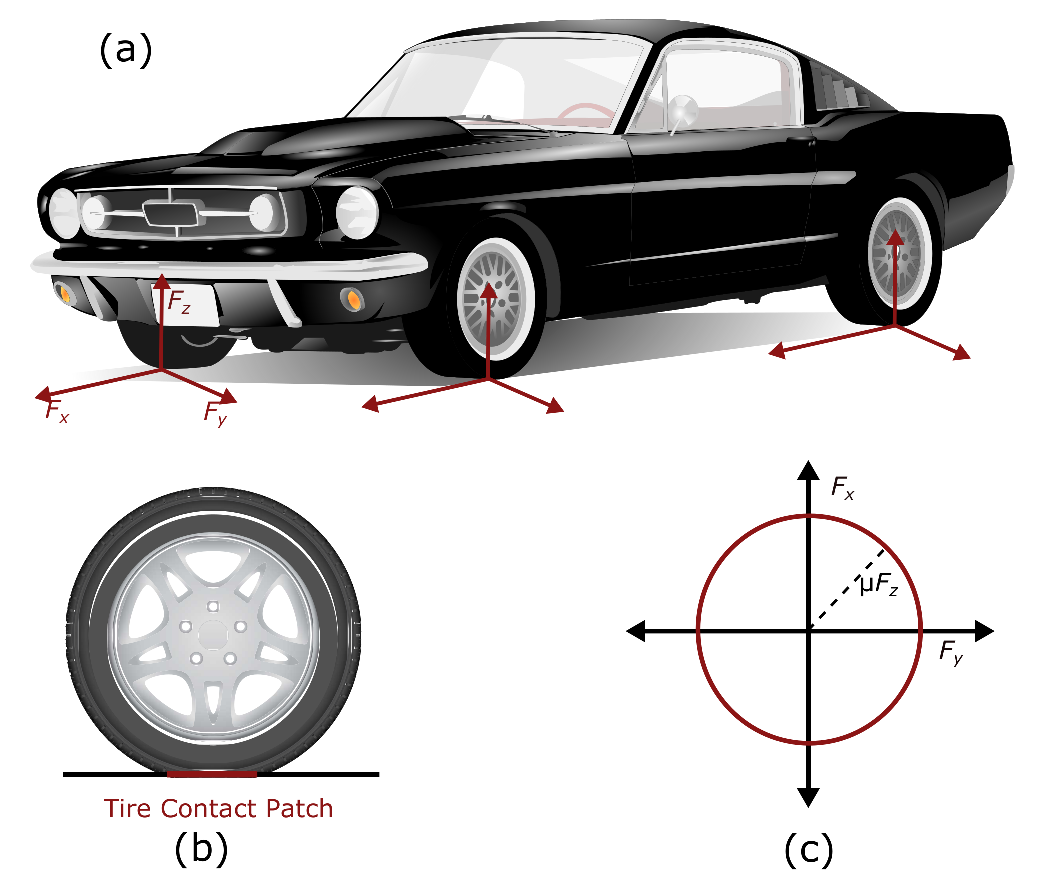
\includegraphics[width= \textwidth]{frictionForces.eps}
\caption[Driving at the limits]{(a) Friction forces $F_x$ and $F_y$ generated in the contact patch allow for lateral and longitudinal vehicle acceleration. (b)
Side view of tire contact patch. (c) Graph showing combined lateral and longitudinal force capability for a tire given the normal load
and friction coefficient $\mu$.}
\label{fig:basicPhysics}
\end{figure}

\subsection{Exceeding the Friction Limits: Understeer and \newline Oversteer}
\label{sec:osteerusteer}
In normal driving situations, the forces required for turning, braking, and accelerating will be much smaller than the
 available friction force. However, in rainy or icy conditions, accidents frequently occur when the driver enters a turn too fast
 or when the driver attempts to turn too quickly while already applying the brakes. In these situations, the tire forces at either the
 front or rear axle become saturated, resulting in one of two distinct scenarios. 

 When the front tires forces become saturated, the vehicle will \textit{understeer}, as illustrated in Fig.~\ref{fig:underover}(a).
 The steering actuator of a vehicle only has direct control of the front tire forces. As a result, 
 additional turning of the steering wheel will not generate additional lateral force or acceleration when the front axle is saturated.
The vehicle therefore becomes uncontrollable and has no ability to reduce the radius of its turn. 
  \begin{figure}[h]
\centering
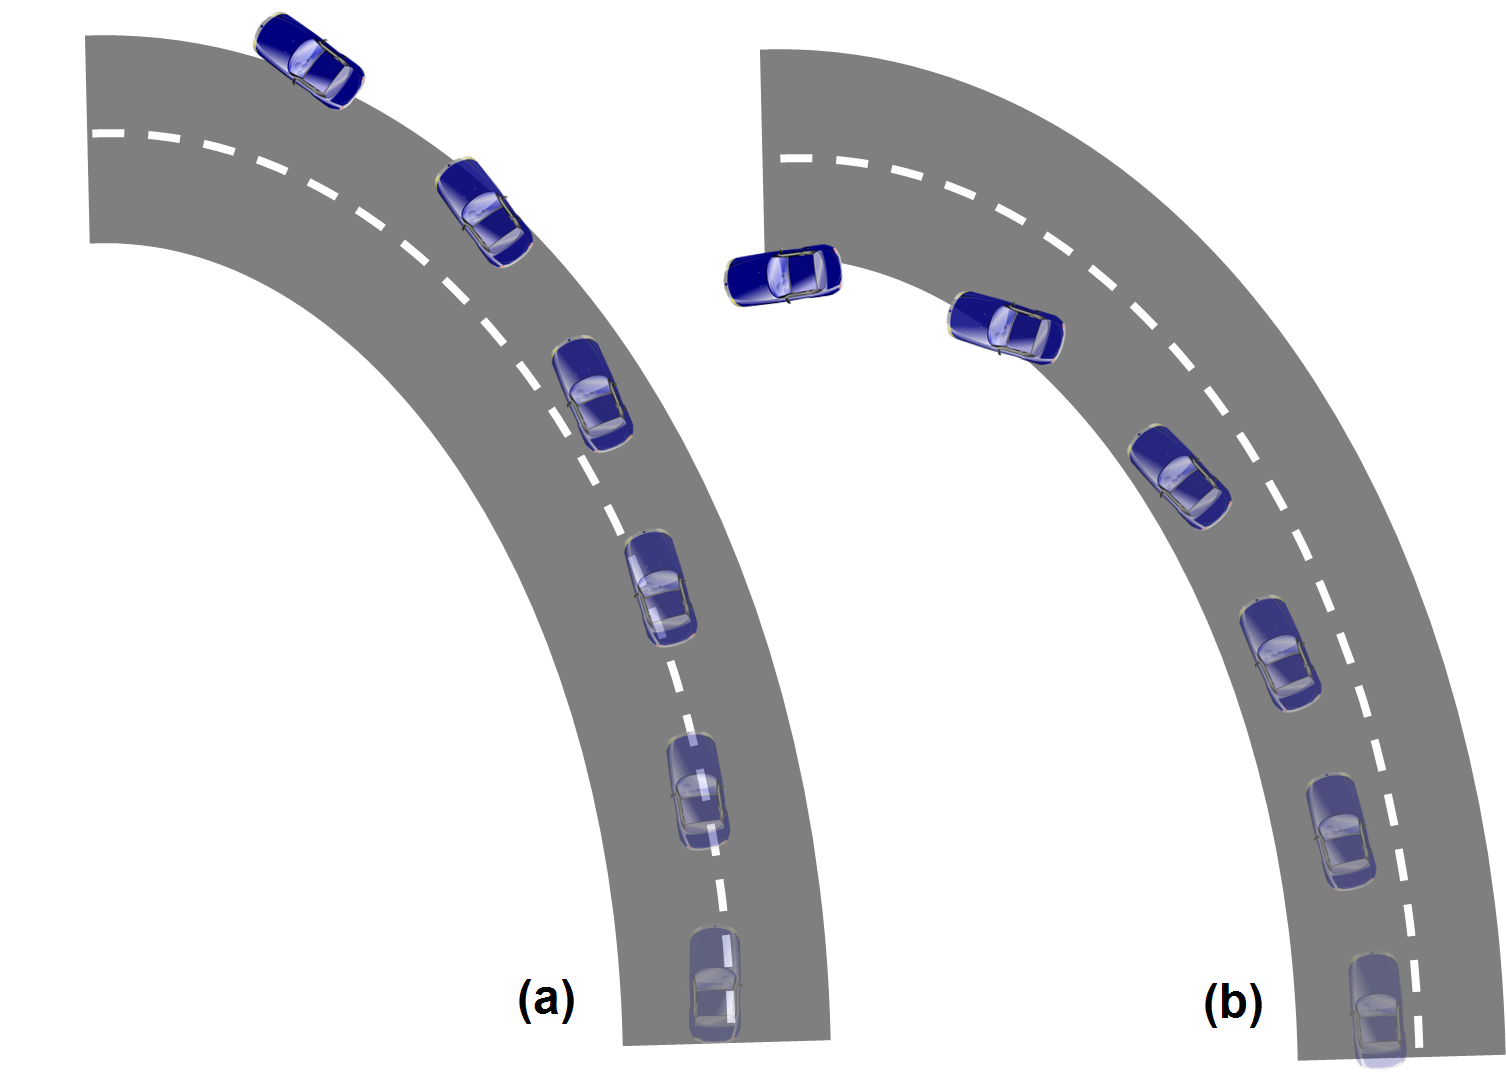
\includegraphics[width= .8\textwidth]{understeeroversteer.png}
\caption[Understeer and Oversteer]{(a) Vehicle understeering at the limits of handling. (b) Vehicle oversteering at the limits of handling.}
\label{fig:underover}
\end{figure}

For the converse scenario where the rear tire forces become saturated, the vehicle
 enters an \textit{oversteer} condition, as illustrated in Fig.~\ref{fig:underover}(b). In this situation, the vehicle loses stability and begins to
spin. An oversteer situation differs
 from an understeer because the front tire forces are not saturated, and the steering actuator can therefore be used to fully control the vehicle. As a result, it is possible
to apply a \textit{countersteer} maneuver to reverse the vehicle spin and gain control of the vehicle without deviating from the desired path.

 % Both conditions are extremely dangerous as they can easily result in the
 % vehicle colliding with a fixed obstacle such as a tree or with another vehicle. In large vehicles such as SUVs, understeer and oversteer
 % can also result in vehicle rollover. 
\section{Race Car Driving as Inspiration for \newline Autonomous Safety Systems}

Automotive engineers today face the challenge of designing autonomous safety systems that can utilize 
the full capabilities of the vehicle's tires in emergency scenarios to avoid accidents and
significant understeer or oversteer. While this is a difficult task, professional race driving provides a source of inspiration for 
designing autonomous safety systems. 

In order to complete a race in minimum time, race car drivers use nearly 100\% of the 
available friction between their vehicle's tires and the road. Professional drivers are extremely skilled at coordinating
 their brake, throttle, and steering inputs to maximize the speed of the vehicle through all corners of a race course while keeping
the vehicle tires within the friction limits. Furthermore, they must achieve this while avoiding collisions with
 other competing drivers who are also driving extremely aggressively. Finally, race car drivers often exceed the friction limits temporarily
 while seeking the fastest lap time, and have the ability to re-stabilize the vehicle from an understeer or oversteer scenario. 
 
\textbf{The primary focus of this dissertation is therefore to develop a set of control algorithms that allow an autonomous vehicle to drive at the handling limits with
the same capability as a professional race driver.} In particular, these algorithms focus on autonomously completing three primary tasks that race car drivers demonstrate with 
proficiency:

\begin{enumerate}
 		
  \item \textbf{Vehicle Steering at the Limits of Handling}. A vital task of racing is steering an automobile through a race course at the handling limits. Given the high lateral
  accelerations required for racing, mitigating vehicle oversteer or understeer is necessary. Good race car drivers have the ability to quickly and aggressively operate the
  steering wheel to complete a turn while maintaining vehicle stability.  
  
  \item \textbf{Finding a Time-Optimal ``Racing Trajectory"}. Given a race track and race vehicle, another fundamental task of racing is determining the fastest
		trajectory, or ``racing line" for the vehicle to follow. Race car drivers are skilled at driving though a race track along a path that enables them to take larger
		radius turns and accelerate aggressively on straight paths, increasing the permissible speed of the vehicle given tire friction constraints.
  
  \item \textbf{Lap-to-Lap Learning}. Finally, most races require the driver to complete many laps around the same race track. Given this repetition, 
	race car drivers have the opportunity to improve their lap times by slightly modifying their driving behavior on each lap to account for observations made during prior laps.
	The ability to learn from prior laps of driving also enables race car drivers to account for changing conditions (e.g. increasing temperatures, tire wear) over the course of a race.
  
\end{enumerate} 

While these tasks may seem specific to the niche field of race car driving, algorithms that enable a vehicle to autonomously drive like a race professional have 
enormous potential for vehicle safety systems. Algorithms that allow for steering at the limits of handling can be vital in piloting a vehicle through
a sudden stretch of icy road during the winter. With a small modification to the objective function, an algorithm that maximizes the turning radius on a race course can 
be used to maximize the distance between a vehicle and oncoming traffic. Learning algorithms that allow more precise driving over a fixed race course can be used to assist
drivers with their daily commute. Potential applications of the developed racing algorithms will be discussed further in the conclusion of this dissertation.

\section{State of the Art}
\label{sec:soa}

There has been significant prior work focused on autonomous steering control at the friction limits, time-optimal trajectory planning, and
iteration-based learning control. This section provides a brief overview of prior work that is relevant to the research contributions presented in this dissertation.

\subsection{Autonomous Race Vehicles}
\label{sec:arv}
Given the highly visible marketing opportunity provided by racing, 
several automotive companies have made notable attempts at racing-inspired 
automated driving. In 2008, BMW introduced the ``Track Trainer", which records race data
collected from a professional driver. To ``replay" the professional's driving autonomously,
the vehicle tracks the pre-recorded speed and racing line with a proportional-derivative
controller for throttle and brake and a dynamic programming algorithm for steering \cite{ttrain}. 
Using pre-recorded inputs allows the controller to naively account for nonlinear vehicle dynamics
at the handling limits, although this approach limits the flexibility of the controller to respond to unpredicted events. 

A second German luxury brand, Audi AG, also launched a collaborative research effort with Stanford University in 2008. 
The collaboration, with which this doctoral research is affiliated, resulted in the development of ``Shelley", an autonomous Audi TTS. Doctoral work by Stanford
 students Theodosis \cite{paulthesis} and Kritayakirana \cite{mickthesis} provided initial forays into 
 racing line generation and trajectory-following algorithms. Notable early accomplishments include autonomous driving
at speeds of 190 mph at the Salt Flats in Utah and an autonomous drive up the Pikes Peak International Hill Climb in 2009 \cite{ppeak}\cite{saltflats}. 
More recently, Audi has incorporated results from the collaboration to build a demonstration vehicle for media events, ``Bobby" (Fig.~\ref{fig:bobby}), 
an autonomous RS7 which debuted at Germany's Hockenheimring \cite{hocky}. The primary focus for the RS7 vehicle was robustness,
enabling the vehicle to be demonstrated at a public event with journalists inside the vehicle at high speeds. 	

 \begin{figure}
\centering
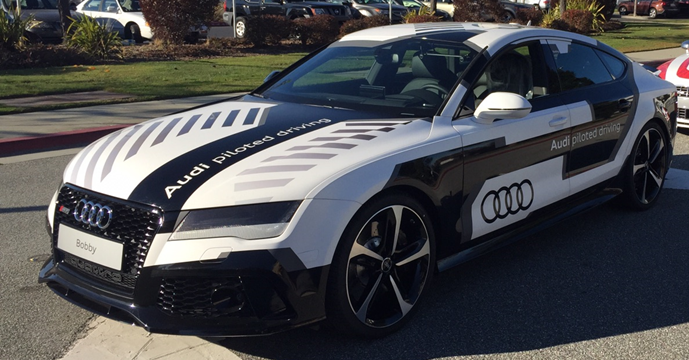
\includegraphics[width= .75\textwidth]{bobby.png}
\caption[Audi's autonomous RS7]{``Bobby", Audi's autonomous RS7.}
\label{fig:bobby}
\end{figure}
 
\subsection{Automated Steering at the Limits of Handling}
\label{pw1}

In the 1990's and early 2000's, a primary focus of autonomous driving research was
designing control systems to follow a desired path \textit{below} the limits of handling. Initial designs typically centered
around linear feedback-feedforward controllers, using linear models of the vehicle dynamics to design the steering control laws \cite{shladover}. An
important development at this time was the idea of \textit{lookahead} steering feedback, where the objective is to 
minimize the lateral tracking error at a certain point in front of the vehicle \cite{guldner}\cite{hingwe}\cite{rosseter}. 

Given the success of linear controller designs for automated steering, early 
attempts at driving at the handling limits also made the assumption of linear vehicle dynamics. While the dynamics of an 
automobile become nonlinear at the handling limits due to tire saturation, assuming linear dynamics in the controller design 
resulted in respectable results in several studies \cite{bessyboy}\cite{sharpysharp}\cite{tommyboy}. To improve upon these results, 
more recent publications have proposed control systems that account for the nonlinear effect of tire saturation at the handling limits
\cite{filho14}\cite{mickcop}\cite{yang14}. The most recent development has been the application of model-predictive control (MPC), which enables
state-of-the-art steering controllers to track a path at the handling limits while trading off between competing objectives of obstacle avoidance and vehicle stabilization \cite{carvalho13}\cite{joethesis}.

While there are a wide variety of published steering controllers with varying levels of complexity, there is no single experimentally validated
controller that displays a well-understood combination of robust stability margins and low path tracking error both at the limits of handling and
in ordinary driving situations. Work by
 Rosseter \cite{rosseter} and Talvala \cite{talvthesis} provides great analysis of the
desirable stability properties of lookahead steering feedback, but no discussion of how path tracking behavior changes as the
vehicle approaches the limits of handling. Kritayakirana and Gerdes \cite{mickcop} 
presented a steering controller with lookahead feedback and a feedforward designed to provide zero lateral error at the vehicle \textit{center of percussion}, a special point within the vehicle frame. 
This method was validated experimentally at the limits of handling and had desirable stability properties, although there was an
issue of competing feedback and feedforward control due to the selection of inconsistent error minimization points. 
Experimentally validated results using model-predictive control \cite{carvalho13}\cite{joethesis} demonstrate the ability to balance competing
objectives of vehicle path tracking and stability when the front or rear tires are saturated, but 
consist of complex optimization problems that make fundamental issues such as stability and closed-loop tracking performance difficult to analyze mathematically or
understand qualitatively. 

\subsection{Time-Optimal Trajectory Planning}
\label{pw2}

The problem of calculating the minimum lap time trajectory for a given vehicle and race track has been studied over the last several decades
in the control, optimization, and vehicle dynamics communities. Early attempts were generally focused on determining analytical
solutions for simple maneuvers via the calculus of variations \cite{hendrikx} or developing qualitative insights for race car drivers and enthusiasts \cite{mken}\cite{taruffi}. With advances in computing power and numerical optimization techniques, 
minimum-time path planning sparked the interest of professional racing teams hoping
to quantitatively determine the effect of vehicle modifications on the optimal lap time for a specific racing circuit. Casanova \cite{casanova} therefore developed a method in 2000 (later 
refined by Kelly \cite{kelly} in 2008) capable of simultaneously optimizing both the path and speed profile
for a fully nonlinear vehicle model using nonlinear programming (NLP). The developed software helped Formula One race teams
analyze the effects of subtle changes in vehicle parameters, including tire thermodynamic properties and suspension designs.

More recently, the development of autonomous vehicle technology has led to research on optimal path
 planning algorithms that can be used for driverless cars. Theodosis and Gerdes published a nonlinear gradient descent approach for determining time-optimal racing lines
 \cite{theodosis}, which has the rare distinction of being validated experimentally on an autonomous race vehicle. 
  
 However, a significant drawback of nonlinear programming solutions is high computational expense. Given the need for real-time trajectory planning in
 autonomous vehicles, there has been a recent interest in finding approximate methods that provide fast lap times with low computational expense. Published methods include formulating the minimum lap time problem
 into a model predictive control (MPC) problem \cite{morari}\cite{timings} or solving a series of locally optimal optimization
 problems \cite{gerdts}\cite{velly}. However, one potential 
 drawback of the model predictive control approach is that an optimization
 problem must be reformulated at every time step, which can still be computationally expensive.
 
 Experimental validation on an 
 autonomous race vehicle has only been reported by Theodosis and Gerdes \cite{theodosis} and Gerdts et al. \cite{gerdts}. 
 To the author's knowledge, a trajectory planning algorithm with a runtime close enough for real-time implementation has not been validated on an experimental vehicle.
 While an autonomous vehicle can apply a closed-loop controller to follow a time-optimal vehicle trajectory computed offline,
 there are  significant benefits to developing a fast trajectory generation algorithm that can approximate the globally optimal trajectory in real-time. 
 If the algorithm runtime is small compared to the actual lap time, the algorithm can run as a real-time trajectory planner and find a fast racing line 
 for the next several turns of the racing circuit. This would allow the trajectory planner to modify the desired path based on the motion of competing race vehicles and 
 estimates of road friction, tire wear, engine/brake dynamics and other parameters learned over several laps of racing. Additionally, the fast trajectory algorithm can
 be used to provide a very good initial trajectory for a nonlinear optimization method.  

\subsection{Iteration-Based Learning}

Developing algorithms that mimic a human's ability to adapt and learn over time has been a focus for researchers in a variety
of fields. In the field of automated control, an interesting approach for adaptation is iterative learning control (ILC), based
on the notion that the performance of a system that executes the
\textit{same task} multiple times can be improved by learning from previous executions \cite{bristow}.
Because iterative learning control works best when learning to follow the same reference trajectory under the same ambient conditions, the most common applications
of ILC are in the field of automated manufacturing. Notable examples include CNC machining \cite{kimdi}, industrial robotics \cite{freeman}\cite{hladowski}, piezolectric stage
positioning \cite{huang}, motor control \cite{mohammad}, and microdeposition \cite{hoelzle}. However, the rise of automated systems outside
factory environments has led to preliminary applications of ILC for ground and air robotics \cite{chen}\cite{purwin}\cite{sun}.

 In the field of computer science, a technique widely used for training in automated systems is \textit{reinforcement learning}.
 Reinforcement learning is similar to iterative learning control in that an automated system overcomes uncertainty in the world by
 gradually learning over multiple trials. However, iterative learning control algorithms typically assume the system is modeled by a 
 discrete (often linear) dynamic system, with uncertainty in the form of an unknown but repeating disturbance. On the other hand, 
 reinforcement learning algorithms act on systems modeled by Markov Decision Processes (MDPs), with the uncertainty typically in
 the form of unknown state transition probabilities and rewards. Furthermore, iterative learning algorithms attempt to gradually
 determine an input \textit{control signal} to overcome the unknown disturbance and provide accurate tracking of a reference trajectory. 
 Reinforcement learning algorithms are more general, and develop a \textit{policy} that maps any state within the MDP to
 an optimal action. 

 Like recent ILC research, reinforcement learning has also been widely investigated for applications in ground and air robotics. 
 In the field of UAV control, Ng et al. presented a reinforcement learning algorithm to learn
a controller for autonomous inverted helicopter flight \cite{ng2006}. There have also
been many publications in the area of robotic motion control. For example, in a modification
of reinforcement learning known as ``apprenticeship learning" Lee et al. presented research
where a robot was able to tie a knot after observing human-guided observations \cite{abbeel}. Finally, in the
area of autonomous vehicles, Lauer presented a reinforcement learning approach to designing a steering
controller for a 1:5 scale RC car \cite{lauer}.

In summary, iteration-based learning algorithms have a rich history of validation on manufacturing and robotic systems. Developing similar
algorithms for an autonomous race vehicle could therefore yield significant benefits. Even with a well-designed trajectory planner
 and path-following controller, there will often be regions of the race track where transient vehicle
 dynamics and unmodeled disturbances result in poor tracking of the optimal trajectory. Furthermore, a major determinant of the 
 optimal trajectory is the friction coefficient between the road and the tires. In reality, this is hard to know ahead
of time beyond a reasonable estimate (e.g $0.95 \leq \mu \leq 1.0$). However, at the limits of handling, small differences in the amount of grip
between the tires and road can result in significant lap time differences. Additionally, turns before a long straight section of track
must be driven more cautiously than series of consecutive turns, because exceeding the friction limit can result in lower top speeds
on the fastest part of the track, significantly increasing lap times. Human drivers
understand this effect well, especially for front-heavy vehicles, and use the term ``slow-in, fast-out" to describe their strategy on crucial turns
before a long straight section. The difficulty of precisely following a racing trajectory at the handling limits and determining the optimal acceleration limits
points to the need for a learning approach that can improve lap time performance over multiple laps of driving.
 
\section{Research Contributions and Outline}
Section \ref{sec:soa} provided a brief overview of the state of the art for the three primary tasks of trajectory planning, trajectory following and
iteration-based learning. Opportunities for important further research in each task were articulated as well. 
This section outlines the primary contributions of this doctoral work for each of these racing-inspired research areas. 

\subsubsection{Chapter 2: A Feedback-Feedforward Steering Controller for Accurate Path Tracking and Stability at the Limits of Handling}

Chapter 2 of this dissertation presents a feedback-feedforward steering controller that maintains vehicle stability at the handling limits
along with strong path tracking performance where physically possible. The design begins by considering the performance of a baseline
controller with a lookahead feedback scheme and a feedforward algorithm based on a nonlinear vehicle handling diagram.
While this initial design exhibits desirable stability properties 
at the limits of handling, the steady-state path deviation increases significantly at highway speeds. 
Results from both linear and nonlinear analyses indicate that lateral path tracking deviations are minimized when vehicle sideslip 
is held tangent to the desired path at all times. Analytical results show that 
directly incorporating this sideslip tangency condition into the steering feedback dramatically improves lateral path tracking, 
but at the expense of poor closed-loop stability margins.  However, incorporating the desired sideslip behavior
into the feedforward loop creates a robust steering controller capable of accurate path 
tracking and oversteer correction at the physical limits of tire friction. Experimental data collected from an 
Audi TTS test vehicle driving at the handling limits (up to 9.5 $\mathrm{m/s^2}$) on a full length race circuit demonstrates the
 improved performance of the final controller design. 

\subsubsection{Chapter 3: A Sequential Two-Step Algorithm for Fast Generation of \newline Vehicle Racing Trajectories}
 \label{ch1FGbenefits}
  
 Chapter 3 presents an iterative algorithm that divides the path generation
 task into two sequential subproblems that are significantly easier to solve than the fully nonlinear lap time optimization. Given an initial path through the race track, the algorithm
 runs a forward-backward integration scheme to determine the minimum-time longitudinal speed profile, subject to
 tire friction constraints. With this speed profile fixed, the algorithm updates the vehicle's path by solving a convex optimization problem 
 that minimizes the curvature of the vehicle's driven path while staying within track boundaries and obeying affine, time-varying vehicle dynamics constraints.
 This two-step process is repeated iteratively until the
 predicted lap time no longer improves. While providing no guarantees of convergence or a globally optimal solution, 
 the approach performs very well when validated on the Thunderhill Raceway
 course in Willows, CA. The predicted lap time converges after four to five iterations, with each iteration over the full 4.5 km race course requiring
 only thirty seconds of computation time on a laptop computer. The resulting trajectory is experimentally driven at the race circuit with
 an autonomous Audi TTS test vehicle, and the resulting lap time and racing line are comparable to both a nonlinear gradient
 descent solution and a trajectory recorded from a professional racecar driver. The experimental results indicate that the proposed method is a viable option for 
 online trajectory planning in the near future.
 
 \subsubsection{Chapters 4 and 5: Iterative Learning Algorithms to Improve Autonomous Driving Performance}
 
This dissertation proposes two sets of learning algorithms that gradually refine the driving performance of the autonomous race car 
over time. Chapter 4 presents an iterative learning control (ILC) formulation to gradually determine the proper steering 
and throttle input for transient driving maneuvers along the race track. Racing is an ideal scenario for ILC because race cars 
drive the same sequence of turns while operating near the physical limits of tire-road friction. 
This creates a difficult to model, but repeatable, set of nonlinear vehicle dynamics and road conditions from lap to lap. 
Simulation results are used to design and test convergence of both a 
 proportional-derivative (PD) and quadratically optimal (Q-ILC) iterative learning controller, and 
experimental results are presented at combined vehicle accelerations 
of up to 9 $\mathrm{m/s^2}$.

Chapter 5 focuses on determining the best value of the friction coefficient $\mu$ for turn-by-turn trajectory planning on the track. Because
the friction coefficient is directly linked to the peak accelerations of the speed profile, locally varying $\mu$ for each turn on the track is a way
to tune the aggressiveness of the planned trajectory. Rather than directly encoding the ``slow-in, fast-out" heuristic that human drivers
typically employ, a learning approach is used to automatically determine the fastest strategy. A small but significant collection of data is gathered
from the autonomous vehicle driving different turns of the track with different values of $\mu$ assumed. From this data, an A* search algorithm
is devised that searches through the data and finds the best value of $\mu$ for each portion of the track in order to globally minimize the resulting
lap time. Key developments of this algorithm include designing an appropriate A* heuristic to minimize the needed computation time and designing the cost
function to account for the physical difficulty of altering the vehicle's trajectory while understeering or oversteering. 


%%% REMOVED FIGURES %%%

 % \begin{figure}
% \centering
% \includegraphics[width= \textwidth]{cars.png}
% \caption[Autonomous vehicle prototypes]{Top two rows: Autonomous vehicle prototypes from the top six global automotive manufacturers by volume. From top left: Toyota, General Motors, Hyundai, Ford, Volkswagen, Nissan. Bottom row:
% prototypes from three non-manufacturers. From left: Automotive suppliers Delphi and Bosch, technology firm Google. Images available from Google Search.}
% \label{fig:autoCars}
% \end{figure}

 % \begin{figure}[h]
% \centering
% \includegraphics[width= \textwidth]{adoptCurve.png}
% \caption[Possible adoption curve for autonomous vehicles]{Possible adoption curve for autonomous vehicles as proposed by Bertoncello and Wee \cite{McK}. There will likely be a significant
% period of time where autonomous vehicles must interact with human-operated vehicles.}
% \label{fig:adoptCurve}
% \end{figure}

 % \begin{figure}[h]
% \centering
% \includegraphics[width= \textwidth]{emergency.png}
% \caption[Possible emergency scenarios for autonomous vehicles]{Possible emergency scenarios requiring autonomous vehicle handling near the limits of tire friction, both for a multi-car
 % and single-car scenario. (a) Suddenly oncoming traffic caused by driver error could require an emergency maneuver at the limits of handling.
 % (b) A patch of ice on the road or other inclement conditions could lead to a rapid decrease in tire friction, quickly bringing an autonomous vehicle to the limits of handling.}
% \label{fig:emergency}
% \end{figure}
\chapter{Feedforward-Feedback Steering Controller} 
\label{chapter2}

 A central control task in the operation of an autonomous vehicle is the ability
to maneuver along a desired path, typically generated by a high-level path planner. As a result, a large research effort has been 
devoted to the subject of active steering control for autonomous or semi-autonomous vehicles. Steering systems based on feedback-feedforward (FB-FFW)
control architectures have been a major focus of research. Early
 work by Shladover et al. \cite{shladover} described a FB-FFW controller where the feedforward
steering angle was determined from path curvature and longitudinal force inputs, and the feedback gains were 
selected from a frequency shaped linear quadratic regulator (FSLQR) designed to
 minimize path tracking error while maintaining good ride quality at different frequencies. Nagai et al. \cite{nagai} also used LQR to design two feedback steering controllers for autonomous path following, with one controller using steer angle as the control input
and the other using steering torque. 

Another simple but effective approach to feedback-feedforward steering control is to design a controller with the objective of
making the lateral tracking error zero at a certain ``lookahead" point in front of the vehicle. Minimization of a lookahead
objective was studied by Hingwe and Tomizuka \cite{hingwe}.
A crucial result was the finding that internal yaw dynamics can be damped at all longitudinal velocities by making the
lookahead point a quadratic function of the vehicle velocity. Rossetter \cite{rosseter} also studied lookahead feedback systems extensively,
and derived a similar controller by minimizing a quadratic potential function of the projected lookahead error. 

While initial work was focused at driving well below the limits of tire friction, several
authors obtained respectable results by applying similar methods for more aggresive maneuvers. M{\"u}ller-Be{\ss}ler 
applied a linear plant inversion method to determine feedforward commands for a Volkswagen Golf attempting an aggressive double lane change
maneuver \cite{bessyboy}. Additionally, Thommyppillai et al. \cite{tommyboy} and Sharp et al. \cite{sharpysharp} used a linear preview controller
to simulate path following of a virtual racecar driver. The tendency for linear controller designs to work reasonably well at the limits
 of handling was partially explained by Talvala et al. \cite{talvala}, who were able to find a Lyapunov function demonstrating stability of lookahead steering feedback 
 even in the presence of significant front and rear tire saturation. 

More recent work has focused on improving control performance by accounting for the nonlinear effect of tire saturation at the handling limits. 
Kritiyikarana and Gerdes \cite{mickcop} proposed a force-based FB-FFW controller with the feedforward steering force
 determined by eliminating the error dynamics about the vehicle's center of percussion. The effect of tire saturation was accounted
 for by inverting a nonlinear vehicle dynamics model to convert the desired steering force to a steer angle input. 
Most recently, the emerging trend of model-predictive control has resulted in steering controllers that 
attempt to track a path at the handling limits while also avoiding obstacles. In 2013, Carvalho et al. \cite{carvalho13} demonstrated a model predictive controller (MPC) 
capable of steering an experimental passenger sedan around obstacles at high speeds on an icy road. The controller was based 
on a nonlinear Ackermann model that was iteratively linearized. A similar affine linearization MPC technique was employed by Funke \cite{joethesis} to demonstrate
a student-built vehicle tracking an oval path at accelerations of 8.5 $\mathrm{m/s^2}$ while avoiding rapidly emerging obstacles.  

In summary, there are a wide variety of published steering controllers with varying levels of complexity. However, there is no
 single experimentally validated controller that displays a well-understood combination of robust stability margins
 and low path tracking error at the limits of handling.  The stability properties of lookahead steering below and at the handling
 limits are demonstrated by Rossetter \cite{rosseter} and Talvala \cite{talvthesis}, but with but no discussion of how
 path tracking behavior changes as the vehicle approaches the limits of handling.
Work presented by Kritayakirana and Gerdes \cite{mickcop} was validated
experimentally and has desirable stability properties, but will exhibit non-zero
 path tracking errors below the handling limits with perfect knowledge of the vehicle dynamics.  
range of vehicle accelerations. Experimentally validated results using model-predictive control \cite{carvalho13}\cite{joethesis} demonstrate the ability to balance competing
objectives of vehicle path tracking and stability when the front or rear tires are saturated, but 
consist of complex optimization problems that make fundamental issues such as stability and closed-loop tracking performance difficult to analyze mathematically or
understand qualitatively. 

This chapter therefore presents the design of a feedback-feedforward steering controller that maintains vehicle stability at the handling limits
along with strong path tracking performance where physically possible. 
 A baseline controller with lookahead steering feedback and feedforward based on vehicle kinematics and steady-state tire forces
 is presented in \S \ref{sec:controllerC2}. By focusing on handling characteristics and vehicle kinematics, the feedforward component is able to
remain consistent with the lookahead objective of the steering feedback.  
Section \ref{sec:predSS} uses steady-state simulation results to show this baseline controller will exhibit 
significant path tracking errors at both low and high vehicle lateral accelerations. 
 In \S \ref{sec:betafb}, we consider a modified steering feedback that aims to keep the vehicle sideslip tangent to the desired path. This approach results
 in a closed-loop steering
response with zero steady-state lateral path deviation, but at the cost of poor stability margins. A better
 design approach, presented in \S \ref{sec:goodFFW}, 
is to incorporate the desired sideslip behavior
as a feedforward input, which significantly improves path tracking while maintaining robust stability margins. 
Section \ref{sec:expresults}  provides experimental path tracking data collected
on an Audi TTS test vehicle at Thunderhill Raceway in Willows, California, with
 combined lateral and longitudinal accelerations up to 9.5 $\mathrm{m/s^2}$. 

 \section{Path Description}
 
The objective of the steering controller presented in this chapter is to follow a path generated by a separate high 
level controller. While there are several ways to mathematically represent the coordinates of a desired path, the controller
design will assume the desired trajectory is defined as a series of curvilinear $\left(s, \kappa(s)\right)$ coordinates, where 
$s$ is the distance along the path and $\kappa(s)$ is the instantaneous path curvature. This coordinate system is chosen
because the curvature of a path is very intuitive to map into a desired lateral vehicle force, and ultimately a desired
vehicle steering input. The chosen path description is illustrated
for a simple path in Figure \ref{fig:pathFig}. 

 \begin{figure}[h]
\centering
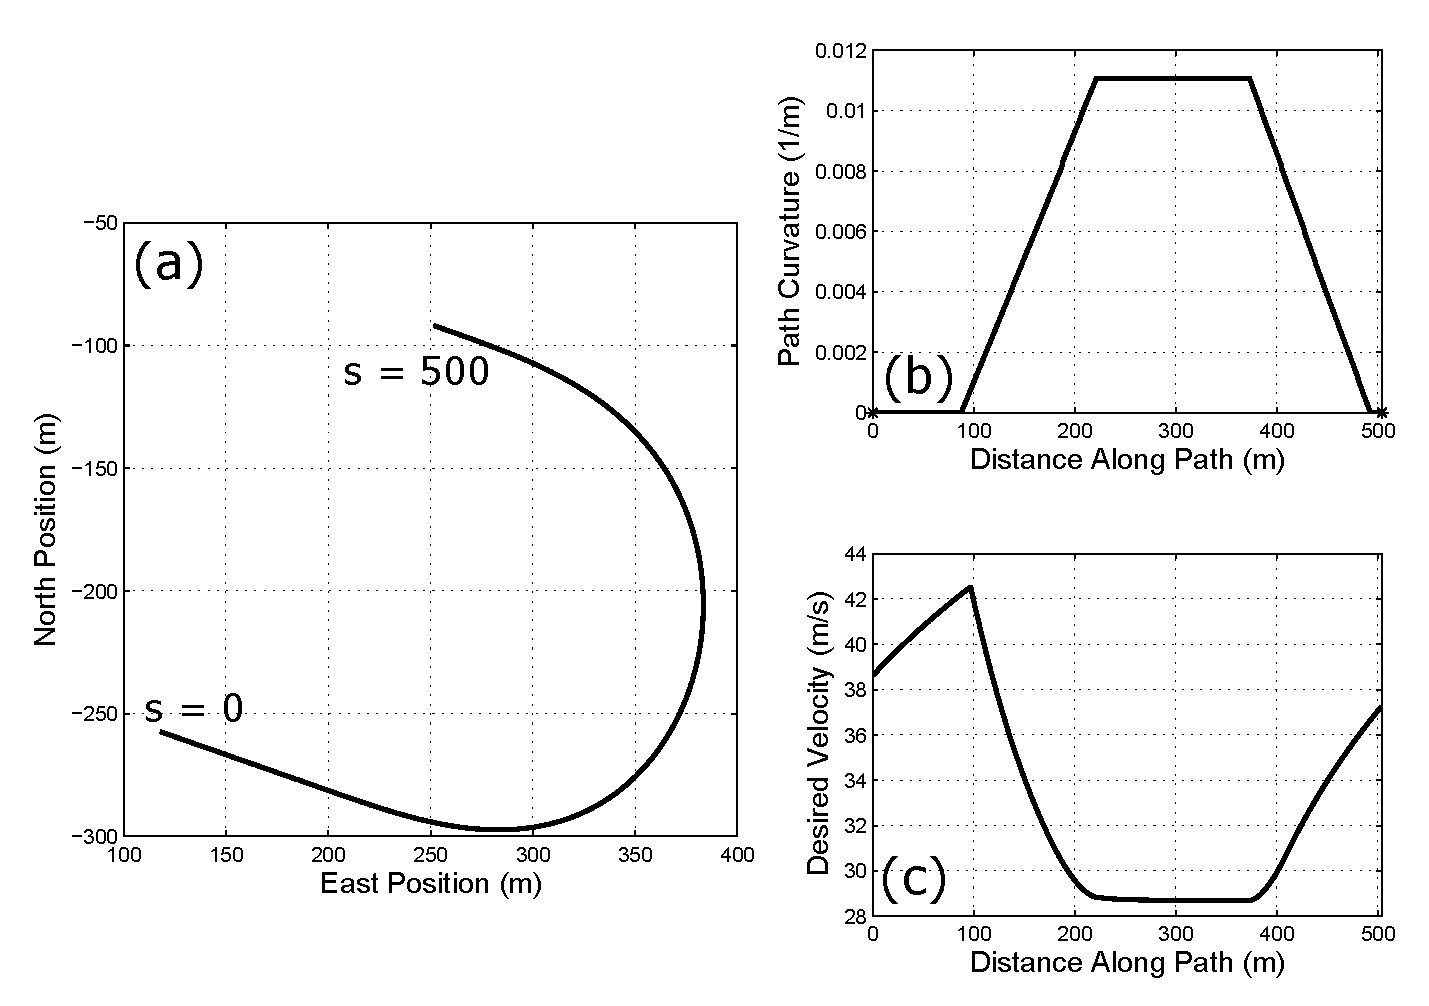
\includegraphics[width=\fullwidth]{pathOverview.eps}
\caption[Path coordinate system]{(a) A 500 meter path plotted in Cartesian coordinates. (b) Curvature profile $\kappa(s)$ as function of 
path length $s$ for associated path. (c) Example velocity profile $(s, U_x^\mathrm{des}(s))$ for path.}
\label{fig:pathFig}
\end{figure}

\newpage
Additionally, given the speed dependence of an automobile's steering dynamics, 
the steering controller also requires knowledge of the desired speed profile (Figure \ref{fig:pathFig}(c)), which must also come from
the high level trajectory planner. The speed profile can be represented as a series of $(s, U_x^\mathrm{des}(s))$ coordinates,
where $U_x^\mathrm{des}(s)$ is the desired speed at a given distance along the path. 
 


%For the experimental data validation presented in this chapter, the desired path curvature is provided to the
% controller via the path planning algorithm  from Theodosis \cite{theodosis}. This algorithm outputs planned trajectories
% where $\kappa$ is a piecewise-linear function of $s$. Additionally, the velocity profile is obtained
% from a longitudinal controller developed by Kritayakirana that keeps the combined vehicle acceleration magnitude at a specified
% value \cite{mickcop}. 
 
\section{Controller Architecture}
\label{sec:controllerC2}

A block diagram of a typical feedback-feedforward structure for steering control is shown in Fig.~\ref{fig:controllerBD}. Inputs to the feedforward
steering angle $\delta_\mathrm{FFW}$ are the current path curvature $\kappa$ and forward velocity $U_x$. Inputs to the feedback steering angle $\delta_\mathrm{FB}$ are lateral path deviation
$e$ and path heading error $\Delta\Psi$ (Fig.~\ref{fig:bikeModel}). The total steering command $\delta$ is the sum of the feedback and feedforward inputs.

% % % % % % % figure, blockdiagram % % % % % % %
\begin{figure}[h]
\centering
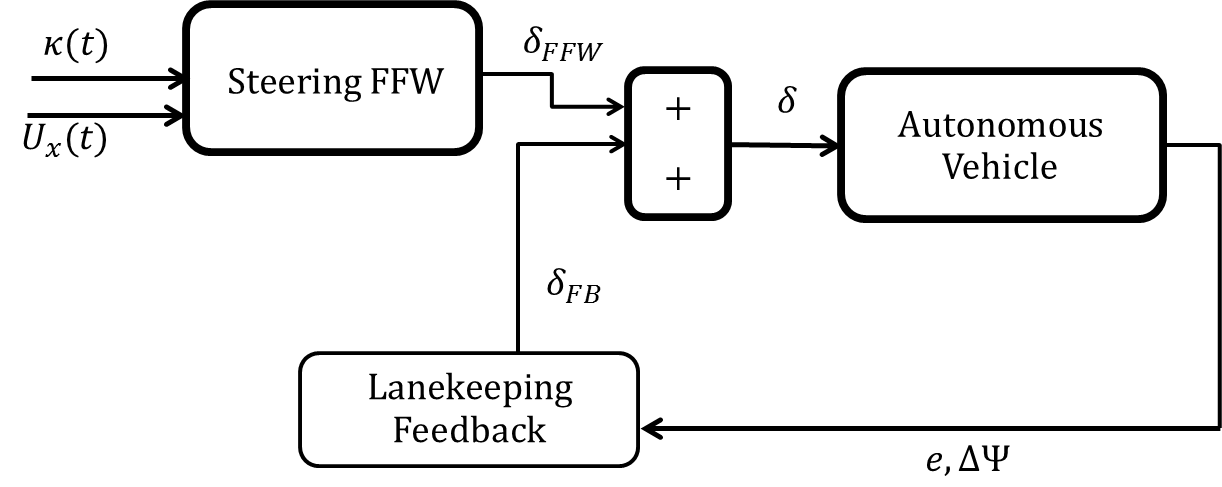
\includegraphics[width=\fullwidth]{FB_FFW.png}
\caption{Block diagram of feedback-feedforward steering controller.}
\label{fig:controllerBD}
\end{figure}
% % % % % % % end figure % % % % % % %

 

\subsection{Feedforward Steering Design}
\label{sec:baselineFFW}

The objective of the steering feedforward is to provide an estimate of the steer angle required to traverse a path with a known path curvature and velocity profile.
This minimizes the level of compensation required by the steering feedback, reducing tracking errors and allowing for less overall control effort. 
To simplify the controller structure, the feedforward steering angle should depend only on the desired trajectory and be independent of the actual vehicle states.

The proposed structure of the steering feedforward begins with the assumption that vehicle dynamics are given by the planar ``bicycle" model,
 with relevant vehicle states and dimensions shown in Fig.~\ref{fig:bikeModel} and described in Table \ref{tb:bikeModelDefns}. The planar bicycle model makes the
key assumption that the left and right tires act to produce a single combined lateral force, resulting
in just two lateral forces $F_\mathrm{yf}$ and $F_\mathrm{yr}$ acting at the front  and rear. Actuation of steer angle $\delta$
at the front tire results in generation of the lateral tire forces through the tire slip angles $\alpha_\mathrm{f}$ and $\alpha_\mathrm{r}$. 
The two resulting states that evolve are vehicle yaw rate $r$, which describes the vehicle angular rotation,
 and sideslip $\beta$, which is the ratio of lateral velocity $U_y$ to longitudinal velocity $U_x$.  
 
  \begin{table}[h]
\begin{center}
\caption{Bicyle Model Definitions}\label{tb:bikeModelDefns}
\begin{tabular}{lcc}
Parameter & Symbol & Units \\\hline
Front axle to CG & $a$ & m\\
Rear axle to CG & $b$  & m\\
Front Lateral Force & $F_\mathrm{yf}$ & N\\
Front Tire Slip     & $\alpha_\mathrm{f}$ & rad \\
Rear Lateral Force & $F_\mathrm{yr}$ & N\\
Rear Tire Slip     & $\alpha_\mathrm{r}$ & rad \\
Steer Angle Input  & $\delta$           & rad \\
Yaw Rate   & $r$ & rad/s \\
Sideslip   & $\beta$ & rad \\
Lateral Path Deviation & $e$ & m \\
Heading Deviation & $\Delta\Psi$ & rad \\
Longitudinal Velocity & $U_x$ & m/s \\
Lateral Velocity & $U_y$ & m/s \\\hline
\end{tabular}
\end{center}
\end{table}
 
 In addition to the two vehicle states $\beta$ and $r$, two additional states are required to describe the vehicle's
 position relative to the desired path. These are also shown in Fig.~\ref{fig:bikeModel}. The lateral path deviation,
 or lateral error, $e$, is the distance from the vehicle center of gravity to the closest point on the desired path. 
 The vehicle heading error $\Delta\Psi$ is defined as the angle between the vehicle's centerline and the tangent line
 drawn on the desired path at the closest point. 
\begin{figure}[h]
\centering
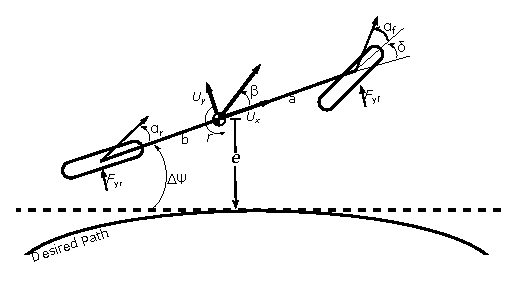
\includegraphics[width=.75\fullwidth]{BikeModelSchematic.eps}
\caption[Schematic of planar bicycle model]{Schematic of planar bicycle model.}
\label{fig:bikeModel}
\end{figure}
Note that the longitudinal dynamics of the vehicle are not explicitly
 modeled in this formulation. Instead of keeping the longitudinal velocity $U_x$ as a vehicle state, the longitudinal
 velocity is treated as a time-varying parameter. 

The problem of determining suitable feedforward lateral tire forces for autonomous path following was studied by Krisada and Gerdes \cite{mickcop}. The (linearized) equations of 
motion for the states shown in Fig.~\ref{fig:bikeModel} are given by:

\begin{subequations}
\label{eq:bm}
\begin{align}
	\dot{\beta} &= \frac{F_\mathrm{yf}+F_\mathrm{yr}}{mU_x} - r \label{eq:bm1}\\
	\dot{r} &= \frac{aF_\mathrm{yf} - bF_\mathrm{yr}}{I_z} \label{eq:bmc2} \\
	\dot{e} &= U_x (\beta + \Delta\Psi) \label{eq:bm3} \\
	\Delta\dot{\Psi} &= r - \dot{s}\kappa \label{eq:bm4} 
\end{align}
\end{subequations}
where $m$ and $I_z$ are the vehicle mass and out-of-plane rotational inertia, and $s$ is the distance along the desired path. Taking time derivatives of $\dot{e}$ and $\Delta\dot{\Psi}$ and substituting from (\ref{eq:bm1}) and (\ref{eq:bmc2}) yields:

\begin{subequations}
\label{eqn:doubleds}
\begin{align}
	\ddot{e} &= \frac{F_\mathrm{yf}+F_\mathrm{yr}}{m} - U_x\kappa\dot{s} \\
	\Delta\ddot{\Psi} &= \frac{aF_\mathrm{yf} - bF_\mathrm{yr}}{I_z} -\kappa\ddot{s} - \dot{\kappa}\dot{s}
\end{align}
\end{subequations}
In general, the values chosen for the feedforward front and rear tire forces $F_\mathrm{yf}$ and $F_\mathrm{yr}$ should
bring $\ddot{e}$ and $\Delta\ddot{\Psi}$ to zero. However, for a typical front-steer vehicle, 
direct control is only available for the front steering force $F_\mathrm{yf}$ via command of the steering input $\delta$. The rear tire
force depends indirectly on the steering angle via the build-up of rear tire slip $\alpha_\mathrm{r}$. It is therefore
not possible to simultaneously eliminate both the lateral tracking error and heading angle error. 

An alternative is to consider eliminating a weighted combination of the two error states by eliminating the lateral tracking 
error $e_p$ at a specified point $x_p$ in front of the vehicle, as shown in Fig.~\ref{fig:projerr}. The error dynamics at this projected point are given by: 

\begin{subequations}
\label{eqn:xp}
\begin{align}
	e_p        &= e + x_p\Delta\Psi \\
	\ddot{e}_p &= \frac{F_\mathrm{yf} + F_\mathrm{yr}}{m} - U_x\kappa\dot{s} + x_p\frac{aF_\mathrm{yf} - bF_\mathrm{yr}}{I_z} - x_p(\kappa\ddot{s} + \dot{\kappa}\dot{s})
\end{align}
\end{subequations}

\begin{figure}[h]
\centering
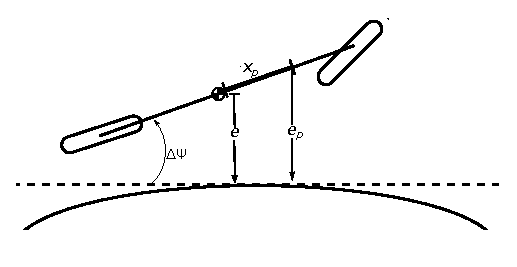
\includegraphics[width=.8\fullwidth]{epfig.eps}
\caption{Projection of lateral error at distance $x_p$ in front of the center of gravity.}
\label{fig:projerr}
\end{figure}

Kritayakirana and Gerdes \cite{mickcop} proposed the center of percussion $x_\mathrm{cop} = \frac{I_z}{bm}$ as a convenient projection point
for the feedforward steering. Substituting $x_p = x_\mathrm{cop}$ and $\ddot{e}_\mathrm{cop} = 0$  yields a simplified equation for the front tire force:

\begin{equation}
\label{eqn:xcop}
 F_\mathrm{yf} = \frac{mb}{L}\left(U_x^2\kappa + x_\mathrm{cop}(\kappa\ddot{s} + \dot{\kappa}\dot{s})\right)
\end{equation}

The benefit of choosing the center of percussion becomes clear in (\ref{eqn:xcop}). The error dynamics at the
center of percussion are independent of the rear tire force, which can be highly transient when the vehicle is cornering near the
limits of handling. This leaves the only control input as $F_\mathrm{yf}$, which can be directly
manipulated by the front wheel steering. 

A feedforward steering approach based on eliminating tracking error at the center of percussion performed well experimentally at lateral accelerations up to
7-8 $\mathrm{m/s^2}$ \cite{mickcop}. However, at higher lateral accelerations, the closed-loop steering response became underdamped, and
the result was significant levels of yaw rate and steering wheel oscillation. This was due to the difficulty of translating a
desired front tire force $F^\mathrm{FFW}_\mathrm{yf}$ into the required steering angle $\delta_\mathrm{FFW}$. 
In general, this relationship is dependent on the vehicle yaw rate $r$ and sideslip $\beta$:

\begin{equation}
\label{eqn:bikeffw}
\delta_\mathrm{FFW} = \frac{U_x\beta + ar}{U_x} - f^{-1}(F^\mathrm{FFW}_\mathrm{yf})
\end{equation}
where $f^{-1}(F_\mathrm{y})$ is an inverse tire model relating tire force to tire slip. This raises the question of 
whether to use actual vehicle states or predicted vehicle states from the bicycle model. Using actual states
results in undesirable coupling between the feedback and feedforward controller and oscillations due to transient vehicle dynamics and 
delays in the steering system, while using predicted states will result in inaccurate tire forces if the vehicle deviates from the desired trajectory.

To eliminate yaw rate oscillation and the dependence on sideslip and yaw rate states,
 we propose simplifying the feedforward tire forces by assuming steady-state cornering conditions. Setting $\dot{s} = U_x$, $\ddot{s} = \dot{\kappa} = 0$
in (\ref{eqn:xcop}) and $\dot{r} = 0$ in (\ref{eq:bm}) yields the following front and rear tire forces:

\begin{subequations}
\label{eqn:ffwforces}
\begin{align}
  F_\mathrm{yf}^\mathrm{FFW} = \frac{mb}{L} U_x^2\kappa\\
   F_\mathrm{yr}^\mathrm{FFW}=\frac{ma}{L} U_x^2\kappa
   \end{align}
\end{subequations}

At steady-state conditions and assuming small angles, the feedforward steering angle of the vehicle relates to the front and 
rear lateral tire slip $\alpha_\mathrm{f}$ and $\alpha_\mathrm{r}$ and path curvature $\kappa$ by vehicle kinematics:

\begin{equation}
\label{eqn:steadyffw}
\delta_{\mathrm{FFW}} = L\kappa - \alpha_\mathrm{f}^\mathrm{FFW}+\alpha_\mathrm{r}^\mathrm{FFW}
\end{equation}
where $\alpha_\mathrm{f}^\mathrm{FFW}$ and $\alpha_\mathrm{r}^\mathrm{FFW}$ are the lumped front and rear feedforward tire slip angles. Notice that
 (\ref{eqn:ffwforces}) and (\ref{eqn:steadyffw}) result in a vehicle feedforward based on a steady-state force balance and vehicle kinematics as opposed
to minimizing error about a point such as the center of percussion (\ref{eqn:xcop}). As a result, there are no compatibility issues
 when combining the feedforward with a lookahead steering feedback. 

The choice of feedforward tire slip angles is related to the tire forces in (\ref{eqn:ffwforces}) via the inverted tire model $f^{-1}(F_\mathrm{y})$. 
To account for saturation of tire force with increasing tire slip magnitude, a single friction coefficient brush Fiala model \cite{Pacejka2012} maps lateral 
tire slip angles into tire force as follows: 
\begin{eqnarray}
\label{eqn:fiala}
	F_\mathrm{y\diamond}&=&\begin{cases} -C_{\diamond}\tan\alpha_\diamond + \frac{C_\diamond^2}{3\mu F_\mathrm{z\diamond}} |\tan\alpha_\diamond| \tan\alpha_\diamond \\ \hspace{10mm}- \frac{C_\diamond^3}{27\mu^2F_\mathrm{z\diamond}^2}\tan^3\alpha_\diamond,
\hspace{8mm}  |\alpha_\diamond| < \arctan{\left(\frac{3\mu F_\mathrm{z\diamond}}{C_\diamond}\right)} \\ \\ -\mu F_\mathrm{z\diamond}\text{sgn} \ \alpha_\diamond, \hspace{36mm} \mathrm{otherwise} \end{cases}
\end{eqnarray}
where the symbol $\diamond \in [\mathrm{f},\mathrm{r}]$ denotes the lumped front or rear tire, $\mu$ is the surface coefficient of friction, and $C_\diamond$ and $F_\mathrm{z\diamond}$ are the corresponding cornering stiffness and normal
load parameters. The cornering stiffnesses and friction coefficient are determined from experimental data taken from a ramp-steer maneuver, as shown in Fig.~\ref{fig:tireCurve}.

\begin{figure}[h]
\centering
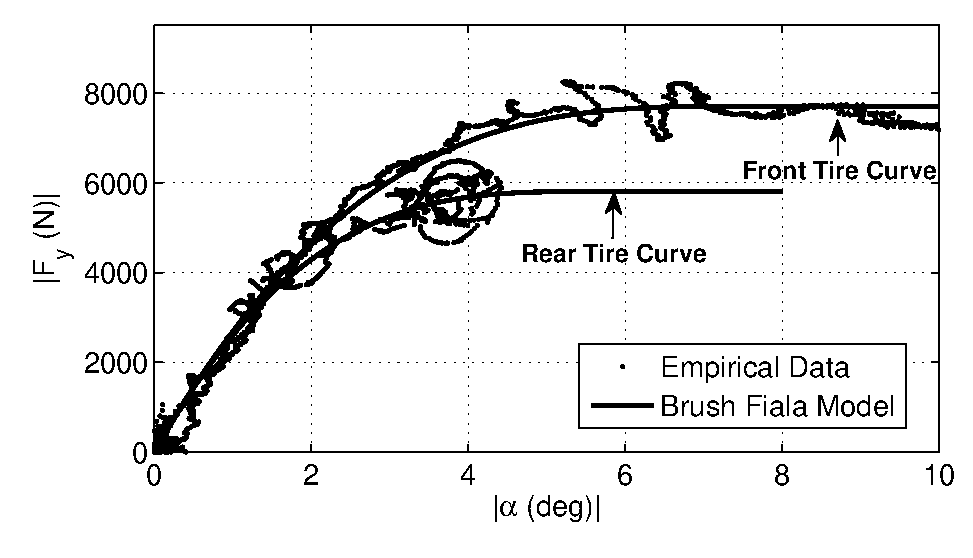
\includegraphics[width=.9\fullwidth]{FrontRearTireCurves.eps}
\caption{Nonlinear tire curves for FFW steering.}
\label{fig:tireCurve}
\end{figure}
\subsection{Feedback Steering Design}
\label{sec:lookahead}

With the feedforward design complete, the remaining step is to design the feedback controller. The goal of the feedback controller is to
minimize a \textit{lookahead} error $e_\mathrm{LA}$, which is the vehicle tracking error projected a distance 
$x_\mathrm{LA}$ in front of the vehicle (Fig.~\ref{fig:lookaheadSchematic}).

\begin{figure}[h]
\centering
\includegraphics[width=.8\fullwidth]{lookaheadSchematic.eps}
\caption{Schematic of planar bicycle model showing projected lookahead error.}
\label{fig:lookaheadSchematic}
\end{figure}

The lookahead error and resulting feedback control law are given by:

\begin{subequations}
\label{eqn:lookahead}
\begin{align}
	e_\mathrm{LA}&=e+x_\mathrm{LA}\Delta\Psi \\
	\delta_\mathrm{FB} &= -k_\mathrm{p}e_\mathrm{LA}
\end{align}
\end{subequations}
with proportional gain $k_\mathrm{p}$. The control law (\ref{eqn:lookahead}) is a natural extension of potential field lanekeeping, as described by Rossetter et al. in \cite{rosseter}, which also provides heuristics for 
selecting $k_\mathrm{p}$ and $x_\mathrm{LA}$. Desirable stability properties of this feedback controller are demonstrated in \cite{talvala}. 

\section{Predicted Steady-State Path Tracking Error}
\label{sec:predSS}

Simulation results provide useful insight about the steady-state path tracking behavior of the baseline feedback-feedforward system. 
Linearized equations of motion for the vehicle and error states can be written in state-space form, with state variable $x$ and control input $\delta$ defined as follows:

\begin{subequations}
\label{eqn:delta}
\begin{align}
		     x &= [e \hspace{2 mm} \Delta\Psi \hspace{2 mm} r \hspace{2 mm} \beta]^T \\
        \delta &=\delta_\mathrm{FB}+\delta_\mathrm{FFW} \\
               &=\left[-k_\mathrm{LK} \hspace{1 mm} -k_\mathrm{LK} x_\mathrm{LA} \hspace{3 mm} 0 \hspace{3 mm} 0\right] x+\left(L+\frac{K_\mathrm{ug} U_x^2}{g}\right) \kappa
\end{align}
\end{subequations}
 where $K_\mathrm{ug}$ is the vehicle understeer gradient, a parameter related to the front/rear weight distribution of the vehicle.
Note that $\delta_\mathrm{FB}$ in (\ref{eqn:delta}b) depends on the state variable, and $\delta_\mathrm{FFW}$ depends on the path curvature. Rewriting  
the vehicle state equations of motion using curvature as the input results in:

\begin{subequations}
\label{eqn:Amatrix}
\begin{align}
    \dot{x} &= Ax + B\kappa  \\
	A  &=  \begin{bmatrix}
   0 & U_x & 0 & U_x \\ 
   0 & 0 & 1 & 0 \\ 
   \frac{-ak_\mathrm{p} C_\mathrm{f}}{I_\mathrm{z}}  & \frac{-ak_\mathrm{p}x_\mathrm{LA}C_\mathrm{f}}{I_\mathrm{z}}  & \frac{-(a^2C_\mathrm{f}+b^2C_\mathrm{r})}{U_xI_\mathrm{z}} & \frac{bC_\mathrm{r} - aC_\mathrm{f}}{I_\mathrm{z}}  \\
   \frac{-k_\mathrm{p}C_\mathrm{f}}{mU_x}  & \frac{-k_\mathrm{p}x_\mathrm{LA}C_\mathrm{f}}{mU_x}  & \frac{bC_\mathrm{r}-aC_\mathrm{f}}{mU_x^2}-1 & \frac{-(C_\mathrm{f} + C_\mathrm{r})}{mU_x}
  \end{bmatrix} \\
	B  &=\left[0 \hspace{2 mm} -U_x \hspace{3 mm} \frac{a C_\mathrm{f} G_\mathrm{FFW}}{I_\mathrm{z}} \hspace{3 mm}  \frac{C_\mathrm{f} G_\mathrm{FFW}}{mU_x}\right]^T
\end{align}
\end{subequations}
where $G_\mathrm{FFW} = (L+\frac{K_\mathrm{ug} U_x^2}{g})$ and $C_\mathrm{f}$ and $C_\mathrm{r}$ are the lumped front and rear cornering stiffnesses. Fig.~\ref{fig:linError} shows results from using the linear model (\ref{eqn:Amatrix}) to compute steady-state path
 tracking errors at the vehicle center of gravity over a range of vehicle speeds, given
 a constant lateral acceleration of $a_y =$ 3 $\mathrm{m/s}^2$. Additionally, steady-state results from the nonlinear feedforward control law 
 (\ref{eqn:steadyffw}) are plotted for the case where $a_y =$ 7 $\mathrm{m/s}^2$. For this high lateral acceleration case, the
 equations of motion (\ref{eq:bm}) and nonlinear Fiala tire model (\ref{eqn:fiala}) are used to predict the steady-state results. In general, steady-state lateral dynamics are reached
within one second for a constant lateral acceleration maneuver. At low lateral accelerations, when the vehicle
 dynamics are dictated by linear equations of motion, the accumulated steady-state tracking error is small ($<$ 0.05 m) at highway speeds. However, 
when steering at the limits of handling, Fig.~\ref{fig:linError} shows that the increased sideslip of the vehicle results
 in higher steady-state tracking error, creating challenges for accurate driving in safety-critical situations. 
 
\begin{figure}[h]
\centering
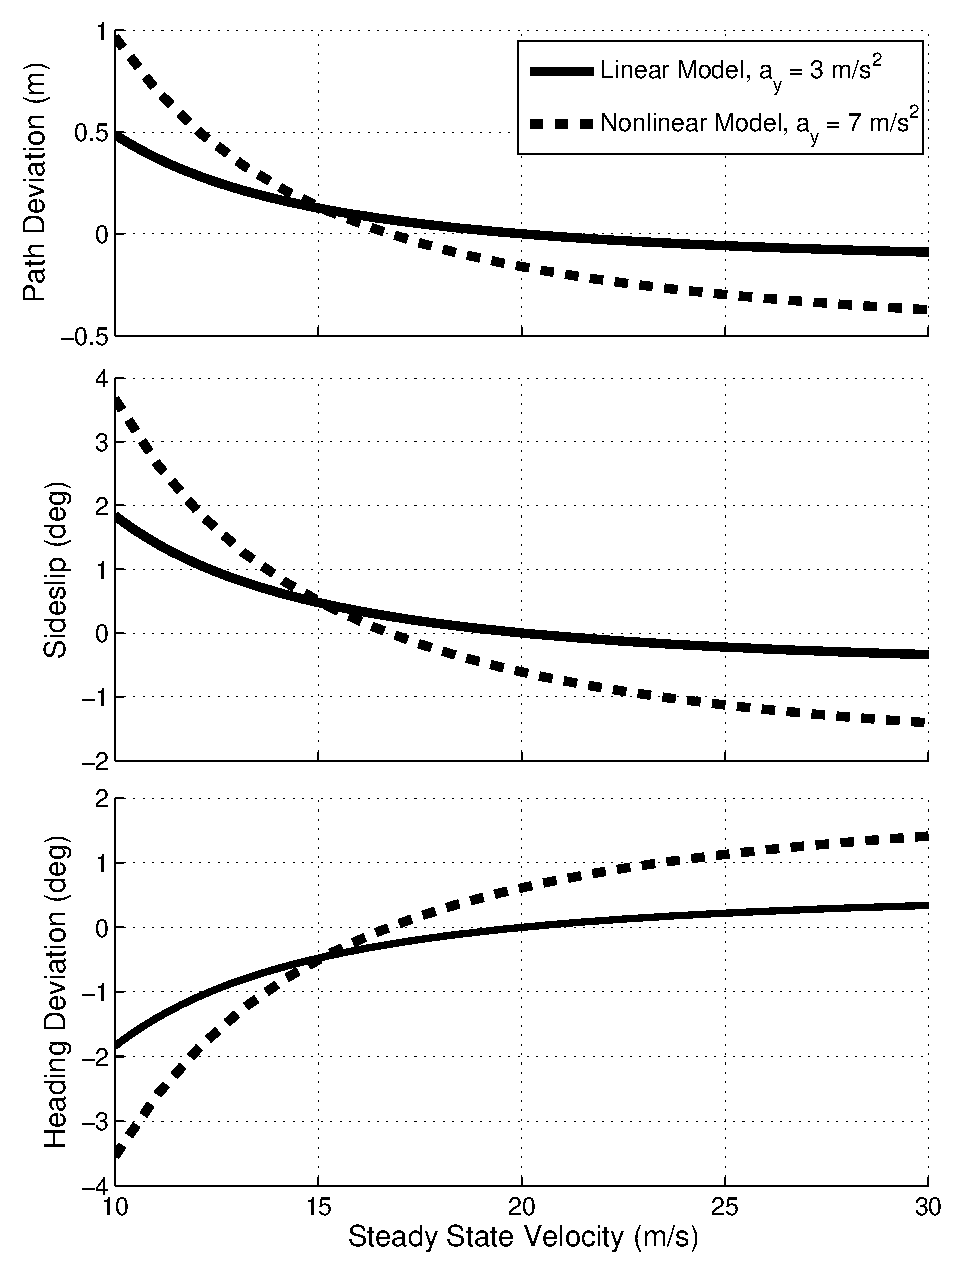
\includegraphics[width=.8\fullwidth]{LinearErrorPlot.eps}
\caption[Steady-state path tracking error $e$, sideslip $\beta$ and heading deviation $\Delta\Psi$ as a function of vehicle speed.]{Steady-state path tracking error $e$, sideslip $\beta$ and heading deviation $\Delta\Psi$ as a function of vehicle speed. Results are plotted for the linear model, with fixed lateral acceleration $a_y = $ 3 $\mathrm{m/s}^2$, and for the
nonlinear model, with fixed lateral acceleration $a_y = $ 7 $\mathrm{m/s}^2$.}
\label{fig:linError}
\end{figure}
 
A qualitative explanation for this steady-state error is shown in Fig.~\ref{fig:SSerror}. Since the steering controller acts to eliminate a weighted
sum of heading error $\Delta\Psi$ and lateral path deviation $e$, the lookahead feedback is successful in
minimizing the desired metric $e_\mathrm{LA}$ at the projected distance $x_\mathrm{LA}$ in front of the vehicle. However, this still allows for steady-state equilibria where
values of $e$ and $\Delta\Psi$ themselves are nonzero.  

\begin{figure}[h]
\centering
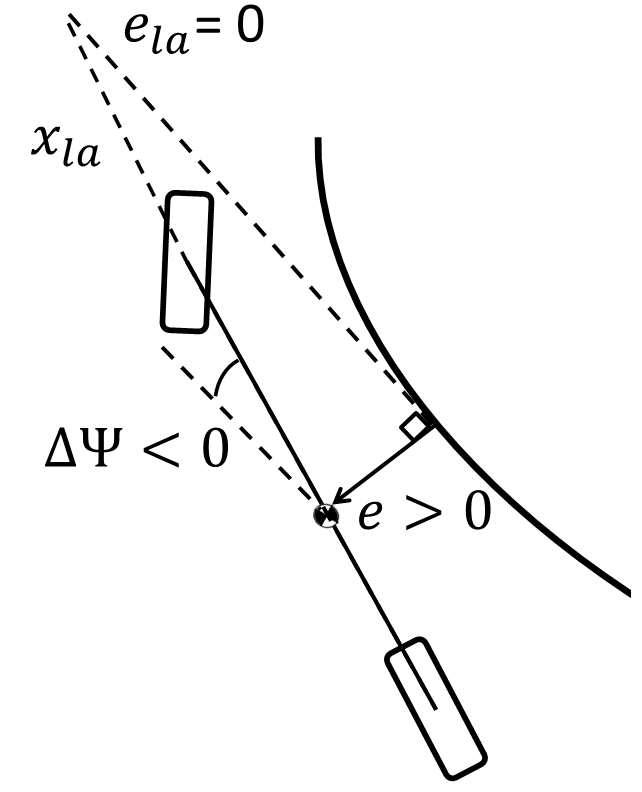
\includegraphics[width=.4\fullwidth]{SSerror.png}
\caption{Steady-state cornering where vehicle has lateral error but no lookahead error.}
\label{fig:SSerror}
\end{figure}
 
% % % % % % % end figure % % % % % % %

%=======================================================================
\section{Incorporating Sideslip-Path Tangency into \newline Steering Feedback}
\label{sec:betafb}

An interesting observation from Fig.~\ref{fig:linError} is that the steady-state path deviation
 is zero at a vehicle speed of around $U_x$=20 m/s for the linear model and $U_x$=17 m/s for the nonlinear model. 
 At these speeds, the steady-state vehicle sideslip is predicted to be zero as well, 
and the vehicle heading $\Psi$ naturally becomes tangent to the desired path heading. 

This observation motivates a second form of lookahead feedback where the feedback objective is to maintain the 
vehicle velocity vector $U = \langle U_x \hspace{2mm} U_y \rangle$ tangent to the desired path, as shown in Fig.~\ref{fig:noSSerror}. Since
 the direction of $U$ is given by $\angle U = \Psi+\beta$, the resulting control law is:
 
\begin{subequations}
\label{eqn:vveq}
\begin{align}
        \delta_\mathrm{FB} & = -k_\mathrm{p} \left(e+x_\mathrm{LA} (\angle U-\Psi_\mathrm{r} ) \right) \\
                           & =  -k_\mathrm{p} \left(e+x_\mathrm{LA} (\Psi+\beta-\Psi_\mathrm{r} ) \right) \\
						   & = -k_\mathrm{p} \left(e+x_{LA}(\Delta\Psi+\beta) \right)
\end{align}
\end{subequations}

 \begin{figure}[h]
\centering
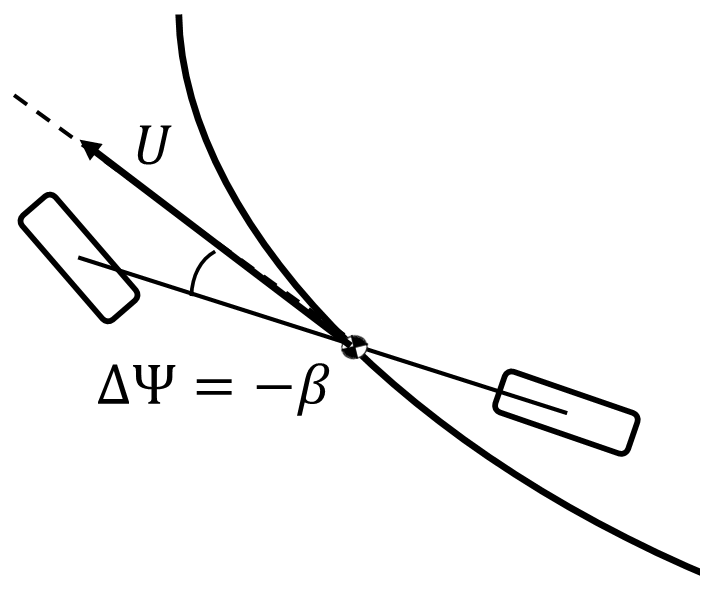
\includegraphics[width=.5\fullwidth]{noSSerror.png}
\caption{Zero steady-state lateral deviation requires vehicle velocity vector
to be tangent to path.}
\label{fig:noSSerror}
\end{figure} 
\noindent where $\Psi_\mathrm{r}$ is the heading of the desired vehicle path at a given point. The modified control law can be modeled by reformulating the matrix $A$ in (\ref{eqn:Amatrix}) as:
 
\begin{equation}
\label{eqn:Amatrix2}
A  = 
 \begin{bmatrix}
  0 & U_x & 0 & U_x \\
  0 & 0 & 1 & 0 \\
  \frac{-ak_\mathrm{p} C_\mathrm{f}}{I_\mathrm{z}}  & \frac{-ak_\mathrm{p}x_\mathrm{LA}C_\mathrm{f}}{I_\mathrm{z}}  & \frac{-a^2C_\mathrm{f}-b^2C_\mathrm{r}}{U_xI_\mathrm{z}} & \mathbf{\frac{bC_\mathrm{r} - aC_\mathrm{f}(1-ak_\mathrm{p}x_\mathrm{LA}) }{I_\mathrm{z}}}  \\
  \frac{-k_\mathrm{p}C_\mathrm{f}}{mU_x}  & \frac{-k_\mathrm{p}x_\mathrm{LA}C_\mathrm{f}}{mU_x}  & \frac{-aC_\mathrm{f}-bC_\mathrm{r}}{mU_x^2}-1 & \mathbf{\frac{-(C_\mathrm{f}(1+k_\mathrm{p}x_\mathrm{LA}) + C_\mathrm{r})}{mU_x}}
 \end{bmatrix}
 \end{equation}
  
Note that (\ref{eqn:Amatrix2}) is equal to (\ref{eqn:Amatrix}b) with the exception of the last column, highlighted
in bold. Fig.~\ref{fig:linError2} shows the resulting steady-state behavior, and indicates that lateral error $e$ settles to
zero for all velocities. 

However, the disadvantage of directly adding vehicle sideslip 
into the feedback control is reduced stability margins. Closed-loop eigenvalues of (\ref{eqn:Amatrix}b) and (\ref{eqn:Amatrix2})
are plotted in Fig.~\ref{fig:rLocusPlot} as a function of increasing vehicle speed from 5 m/s to 25 m/s.
\begin{figure}[h]
\centering
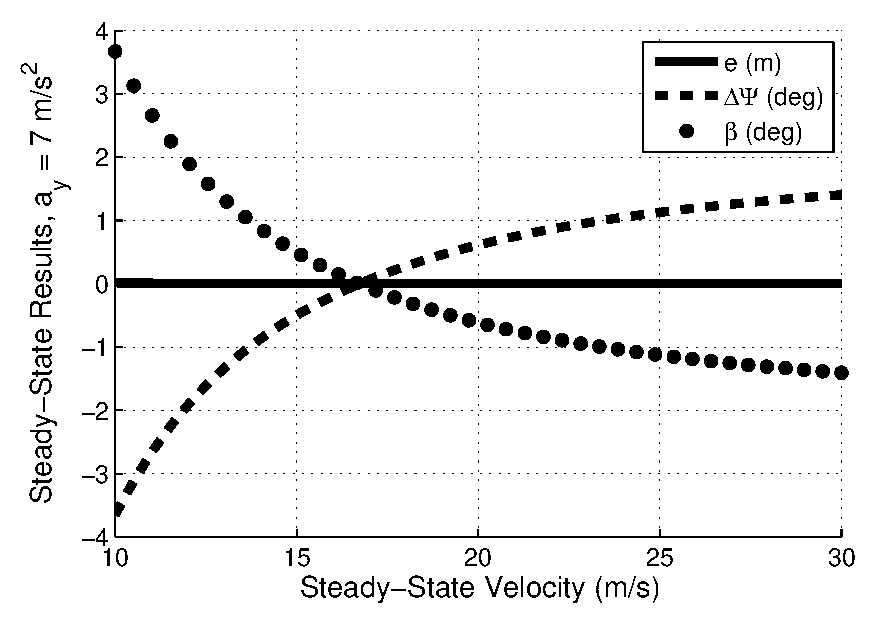
\includegraphics[width=.85\fullwidth]{LinearErrorPlotBeta.eps}
\caption[Steady-state simulation results with sideslip added to feedback control]{Steady-state simulation results with sideslip added to feedback control, using the nonlinear vehicle model with fixed lateral acceleration of 7 $\mathrm{m/s^2}$.}
\label{fig:linError2}
\end{figure} 

The results indicate that the closed-loop steering response
is well-damped ($\zeta =$ 0.9 at a vehicle speed of 25 m/s) with the original lookahead feedback controller. However, when, the steering feedback acts to 
keep the vehicle sideslip tangent to the desired path via (\ref{eqn:vveq}), the closed-loop steering response becomes highly underdamped 
\mbox{($\zeta$= 0.2 at $U_x$ = 25 m/s)}.  

\begin{figure}[h]
\centering
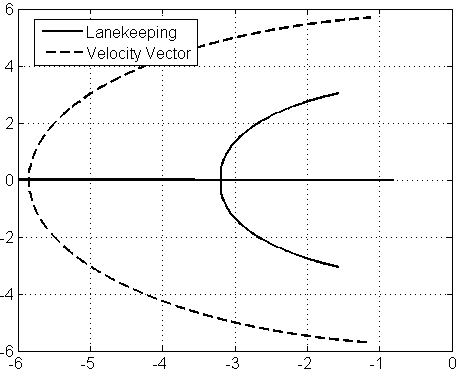
\includegraphics[width=.53\fullwidth]{rLocus.eps}
\caption[Closed-loop pole locations for steering system as vehicle speed is varied from 5 to 25 m/s]{Closed-loop pole locations for steering system as 
vehicle speed is varied from 5 to 25 m/s. Damping ratio $\zeta$ and natural
frequency $\omega_n$ are shown for $U_x$ = 25. Root locus plots are shown for both the lookahead feedback controller (\ref{eqn:Amatrix}) as well as the feedback controller with added
sideslip (\ref{eqn:Amatrix2}). Root locus moves in direction of arrows as vehicle speed is increased.}
\label{fig:rLocusPlot}
\end{figure}
\newpage
Note that the results shown in Fig.~\ref{fig:rLocusPlot} are for a single vehicle and controller parameterization (see Table 1). 
In general, the reduction in stability margin will vary significantly depending on the vehicle understeer gradient and steering controller gains, namely
the lookahead distance. Fig.~\ref{fig:VcrPlot} shows the critical speed $V_\mathrm{cr}$, beyond which the closed-loop 
steering system becomes unstable, for neutral, understeering, and oversteering configurations as a function of $x_\mathrm{LA}$.
For an understeering vehicle, lookahead feedback is always stable as long
as the lookahead point $x_\mathrm{LA}$ is above a certain critical value (a conclusion derived in \cite{rosseter}).   
\begin{figure}[h]
\centering
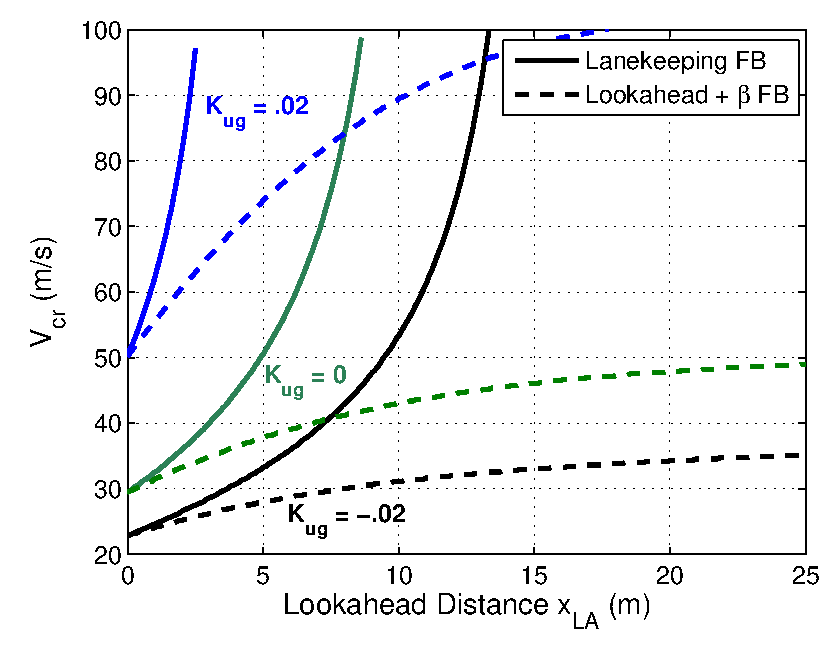
\includegraphics[width=\fullwidth]{VcrPlot.eps}
\caption[Maximum speed for closed-loop stability for the original lookahead feedback and the modified feedback with sideslip tracking.]{Maximum speed for closed-loop stability for the original lookahead feedback and the modified feedback with sideslip tracking. Results are based on
eigenvalue computations of the $A$ matrix of the linear vehicle model.}
\label{fig:VcrPlot}
\end{figure} 
Even in situations where the vehicle is in a 
neutral steer or oversteer configuration, the critical speed for closed-loop stability increases rapidly with lookahead distance. A different trend is present when
sideslip tracking is added to the steering feedback. Fig.~\ref{fig:VcrPlot} shows that the critical speeds for 
stability increase very slowly as a function of lookahead distance.

\section{Incorporating Sideslip Information Into \newline Steering Feedforward}
\label{sec:goodFFW}
 
 Given the trade-off between path tracking and stability when sideslip-path alignment is enforced via feedback, a promising approach
 is to replace vehicle sideslip  $\beta$ in (\ref{eqn:vveq}) with the predicted steady-state sideslip value $\beta_\mathrm{ss}$ 
 for a given vehicle speed and curvature. 

The rear tire slip for a fixed track vehicle, assuming small angles, is given by 
\begin{equation}
\alpha_\mathrm{r} = \beta - \frac{br}{U_x}
\end{equation} 
At steady-state, $\alpha_\mathrm{r}=\alpha_\mathrm{r}^\mathrm{FFW}$ from (\ref{eqn:steadyffw}) and $r=\kappa U_x$, yielding the following feedback control law:
\begin{subequations}
\begin{align}
\label{eqn:betass}
\delta_\mathrm{FB} &=-k_\mathrm{P} \left(e+x_\mathrm{LA} (\Delta\Psi+\beta_\mathrm{ss}) \right) \\
\beta_\mathrm{ss}  &= \alpha_\mathrm{r}^\mathrm{FFW} + b\kappa
\end{align}
\end{subequations}
The effect of this change is to remove the steering controller's dependence on \textit{real-time} sideslip information. The steering
controller will now act to align the vehicle's predicted \textit{steady-state} sideslip along the desired path. Since the controller no
longer has feedback on vehicle sideslip, the state matrix equation $A$ for the closed-loop system dynamics is now 
once again given by (\ref{eqn:Amatrix}b), which was shown to have desirable stability
properties as a function of $K_\mathrm{ug}$ and $x_\mathrm{LA}$ (Fig.~\ref{fig:VcrPlot}). The sideslip now affects the vehicle
path tracking dynamics through the feedforward path, since the predicted steady-state sideslip $\beta_{ss}$ depends only on the
desired speed $U_x$ and curvature $\kappa$ as well as the feedforward tire model. 

The $B$ matrix in (\ref{eqn:Amatrix}) now becomes: 

\begin{subequations}
\label{eqn:newB}
\begin{align}
	B &=\left[0 \hspace{2 mm} -U_x \hspace{3 mm} \frac{a C_\mathrm{f} (G_\mathrm{FFW}+G_\beta)}{I_\mathrm{z}} \hspace{3 mm}  \frac{C_\mathrm{f} (G_\mathrm{FFW}+G_\beta)}{mU_x}\right]^T \\
	G_\beta &= U_x^2\frac{ma}{L}\frac{k_\mathrm{p}x_\mathrm{LA}}{C_\mathrm{r}}
\end{align}
\end{subequations}

Assuming perfect knowledge of the feedforward tire model, the resulting steady-state lateral path deviation will be zero at all vehicle speeds,
as shown in Fig.~\ref{fig:linError2}.
\begin{figure}[h]
\centering
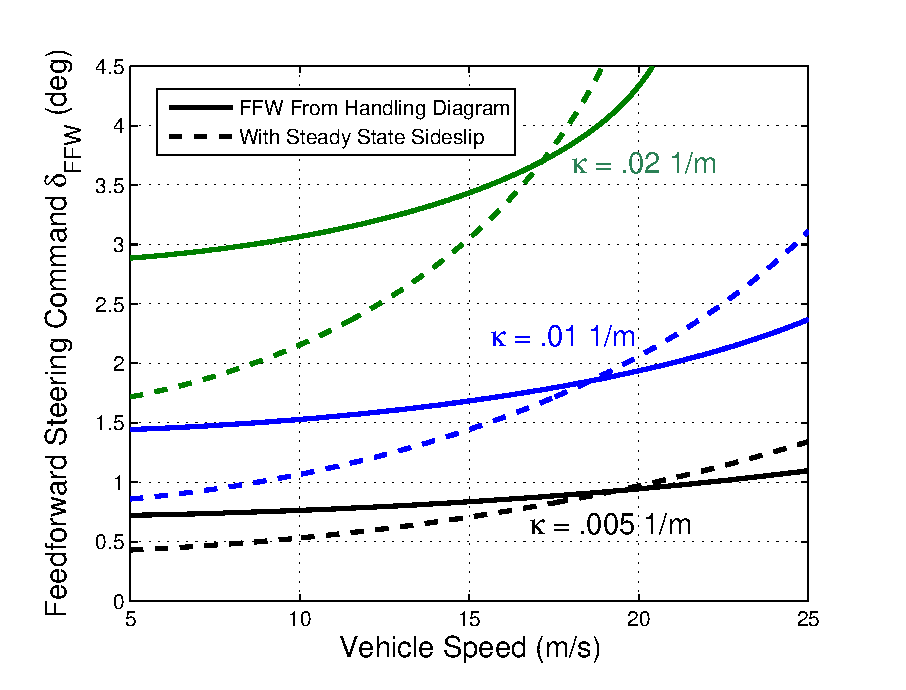
\includegraphics[width=\fullwidth]{FFWplot.eps}
\caption{Effect of incorporating sideslip behavior into feedforward steering command $\delta_\mathrm{FFW}$, as a function of 
vehicle speed and desired path curvature.}
\label{fig:ffwplot}
\end{figure}
However, error in the feedforward tire model will result in steady-state lateral path deviation.
The effect of incorporating steady-state sideslip into the feedforward control is shown in Fig.~\ref{fig:ffwplot}. The feedforward
steering command $\delta_\mathrm{FFW}$ as a function of path curvature and vehicle speed is plotted both for the original feedforward control law (\ref{eqn:Amatrix}c) as well as the sideslip-incorporating
feedforward command (\ref{eqn:newB}). 

\section{Experimental Results}
\label{sec:expresults}

\subsection{Experimental Setup}

Experimental data was collected on ``Shelley", an Audi TTS equipped 
with an electronic power steering motor for autonomous steering and active brake booster and throttle by wire for
longitudinal control (Fig.~\ref{fig:shelleyPicC2}). The testbed is also
equipped with an integrated Differential Global Positioning System (DGPS) and Inertial Measurement Unit (IMU) in order to obtain
 global vehicle states. Mentioned previously in \S \ref{sec:arv}, this is the same vehicle developed by
Stanford and Audi to autonomously drive the Utah Salt Flats and Pikes Peak Hill Climb \cite{saltflats}. 

\begin{figure}[h]
\centering
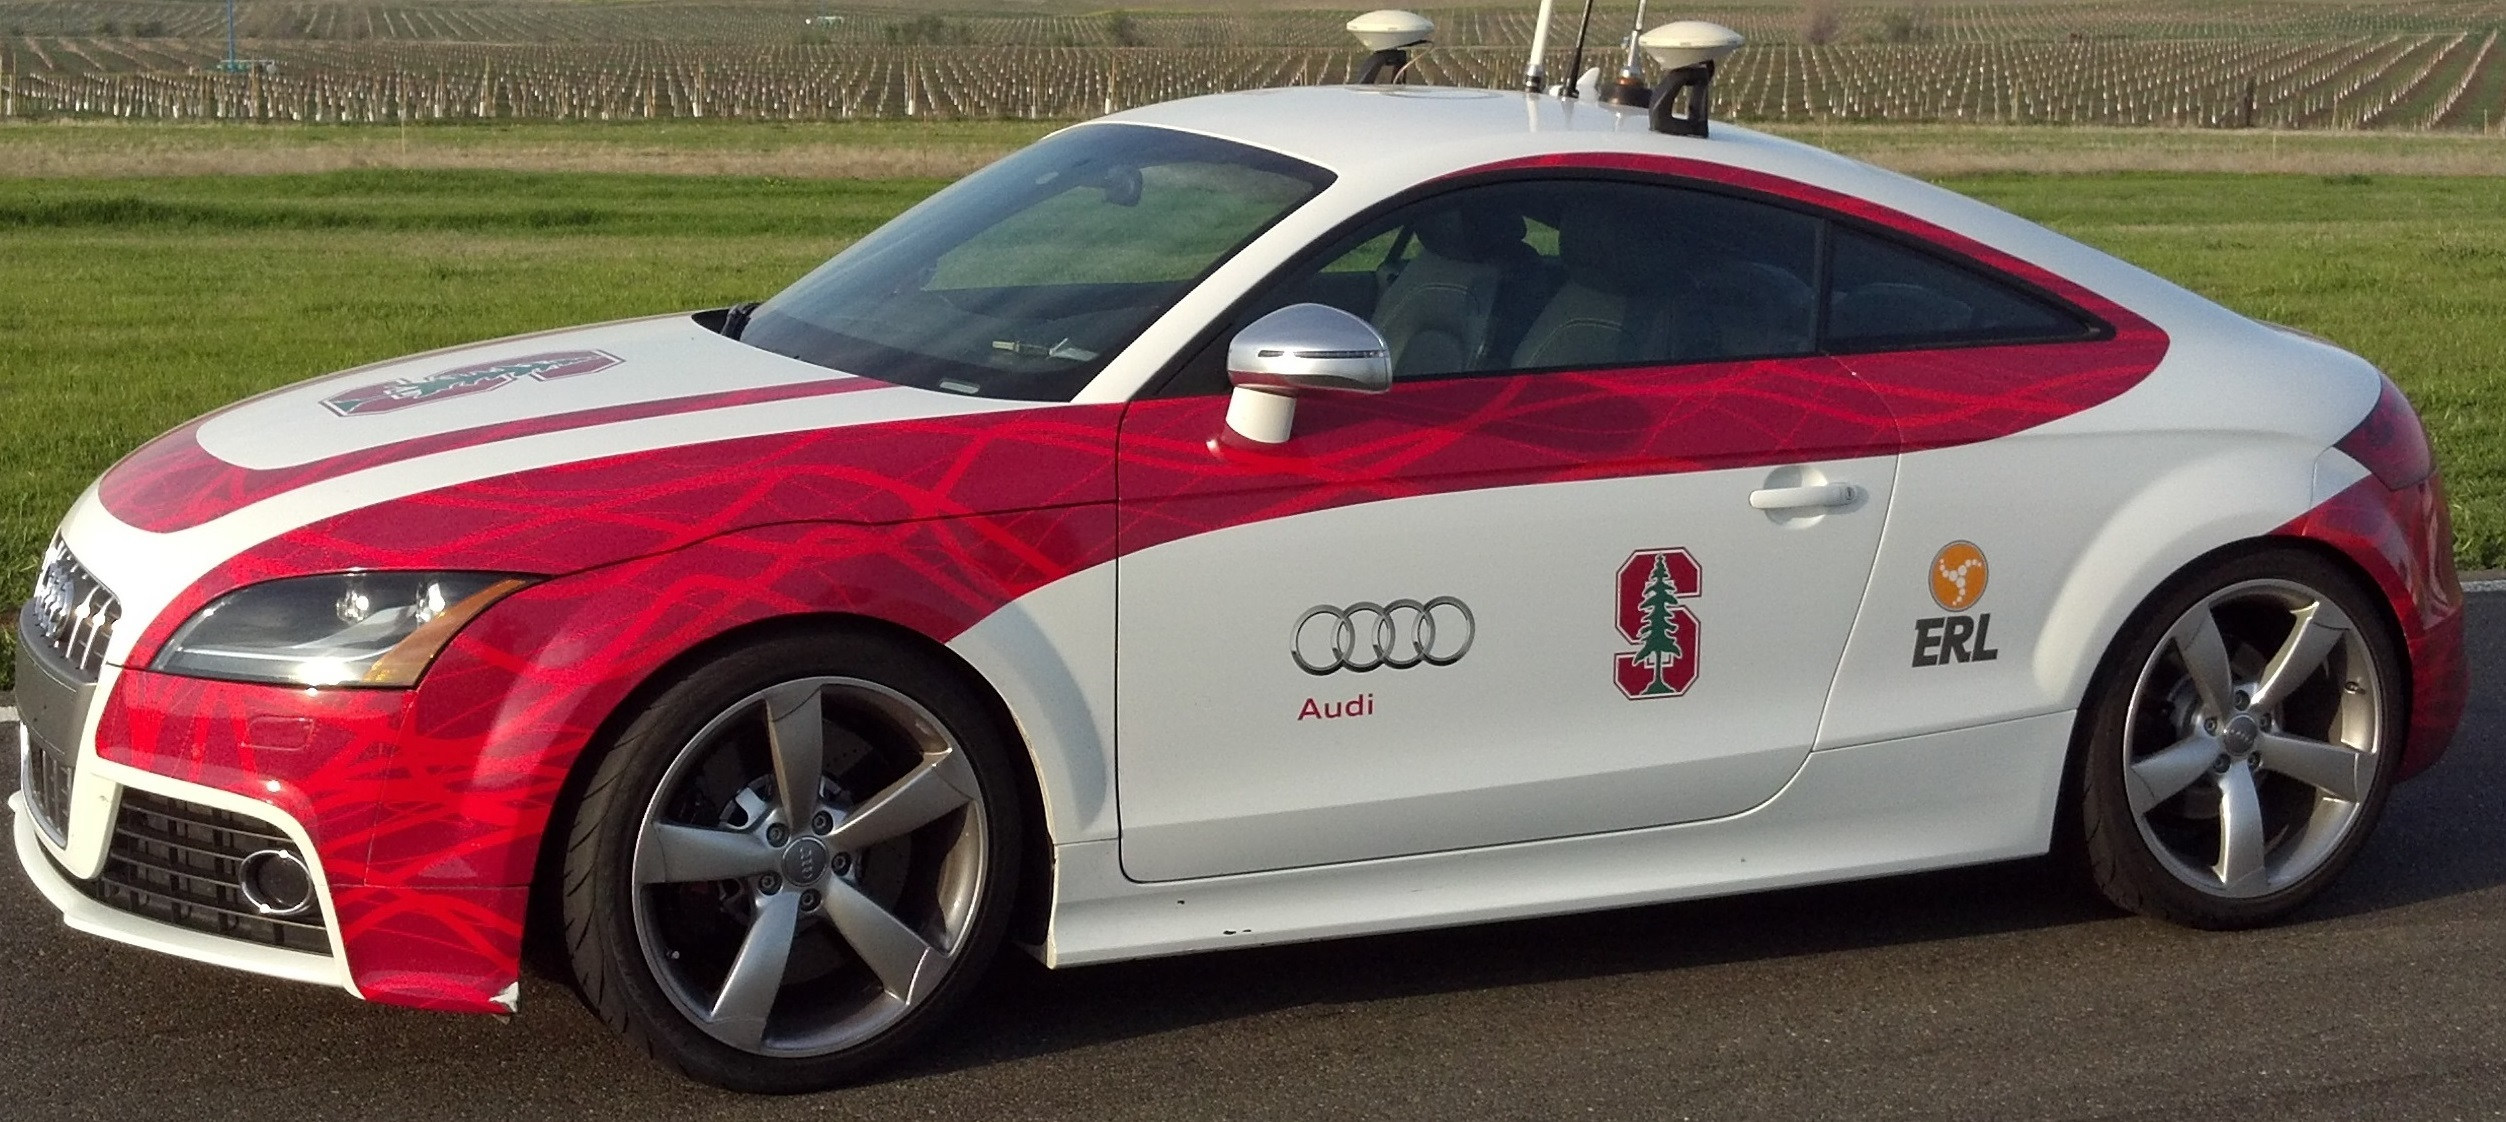
\includegraphics[width=\fullwidth]{experimentInfo.jpg}
\caption{Audi TTS used for experimental validation.}
\label{fig:shelleyPicC2}
\end{figure}

\begin{figure}[h]
\centering
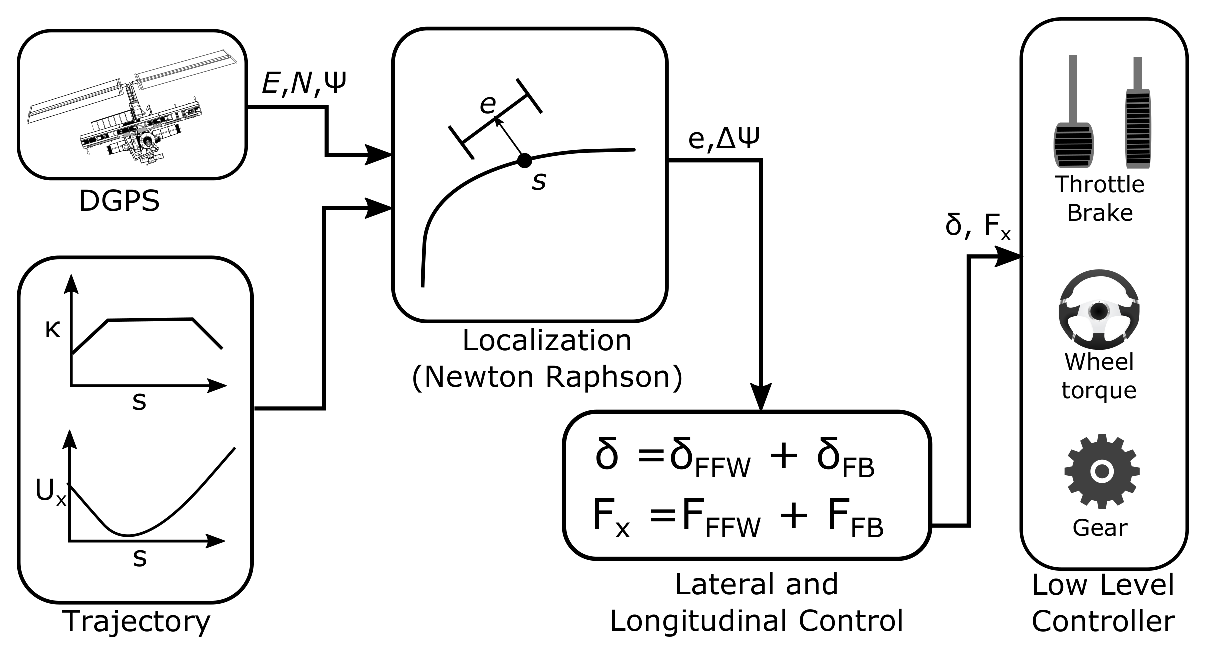
\includegraphics[width=.85\fullwidth]{expSetupC2.eps}
\caption{Diagram showing controller setup.}
\label{fig:expSetupC2}
\end{figure}
\newpage 
The overall controller setup is shown in Fig.~\ref{fig:expSetupC2}. At each time step,
the differential GPS unit obtains precise ( $<$ 2 cm) measurements of the vehicle
 global East and North coordinates as well as the vehicle angular orientation $\Psi$.
 The controller also has prior knowledge of the desired high level trajectory, 
 consisting of the clothoid curvature profile from Theodosis \cite{theodosis} and 
 the speed profile from Kritayakirana \cite{mickthesis}. 
Vehicle parameters for the Audi test vehicle and the lookahead feedback
 gains are presented in Table \ref{tb:params}.

 
 \begin{table}[h]
\begin{center}
\caption{Vehicle Parameters}\label{tb:params}
\begin{tabular}{lccc}
Parameter & Symbol & Value & Units \\\hline
Vehicle mass & $m$ & 1500 & kg \\
Yaw moment of inertia & $I_z$ & 2250 & $\mathrm{kg \cdot m}^2$\\
Front axle to CG & $a$ & 1.04 & m\\
Rear axle to CG & $b$ & 1.42 & m\\
Front cornering stiffness & $\mathrm{C}_\mathrm{f}$ & 160 & $\mathrm{kN \cdot rad}^{-1}$ \\
Rear cornering stiffness & $\mathrm{C}_\mathrm{r}$ & 180 & $\mathrm{kN \cdot rad}^{-1}$ \\
Lookahead Distance		 & $x_\mathrm{LA}$         & 14.2 & $\mathrm{m}$ \\
Lookahead Gain         & $k_\mathrm{p}$         & 0.053 & $\mathrm{rad/m}$ \\\hline
\end{tabular}
\end{center}
\end{table}
 \newpage
 The global East, North, and $\Psi$ measurements
are fed into a Newton-Raphson localization algorithm, which finds the closest point from the vehicle
center of gravity to the path and outputs values of $e$ and $\Delta\Psi$. The resulting steering
command is generated using the feedback-feedforward control laws developed in this chapter. 
In addition, to track the desired speed profile, a longitudinal force command is generated with a basic 
proportional control law presented by Kritayakirana \cite{mickthesis}. Finally, a low level
controller developed by Audi and Stanford maps the
steer angle and force command into the resulting throttle, brake, steering wheel torque, and gear shift commands.  
The control loop operates at 200 Hz, with computations performed on a dSPACE MicroAutobox real-time embedded computer. 

The site for data collection was a 3.1 mile paved racing circuit (friction coefficient $\mu \approx$ 1) at Thunderhill Raceway Park in Willows, CA.
Fig.~\ref{fig:thPic} shows an overhead plot of the race track as well as the desired racing line. The desired racing
line is parameterized as a curvature profile $\kappa(s)$ that varies with distance along the path. The curvature
profile associated with the racing line is shown in Fig.~\ref{fig:traj}
along with a typical longitudinal velocity profile $U_x$ from the path planner.

\begin{figure}[h]
\centering
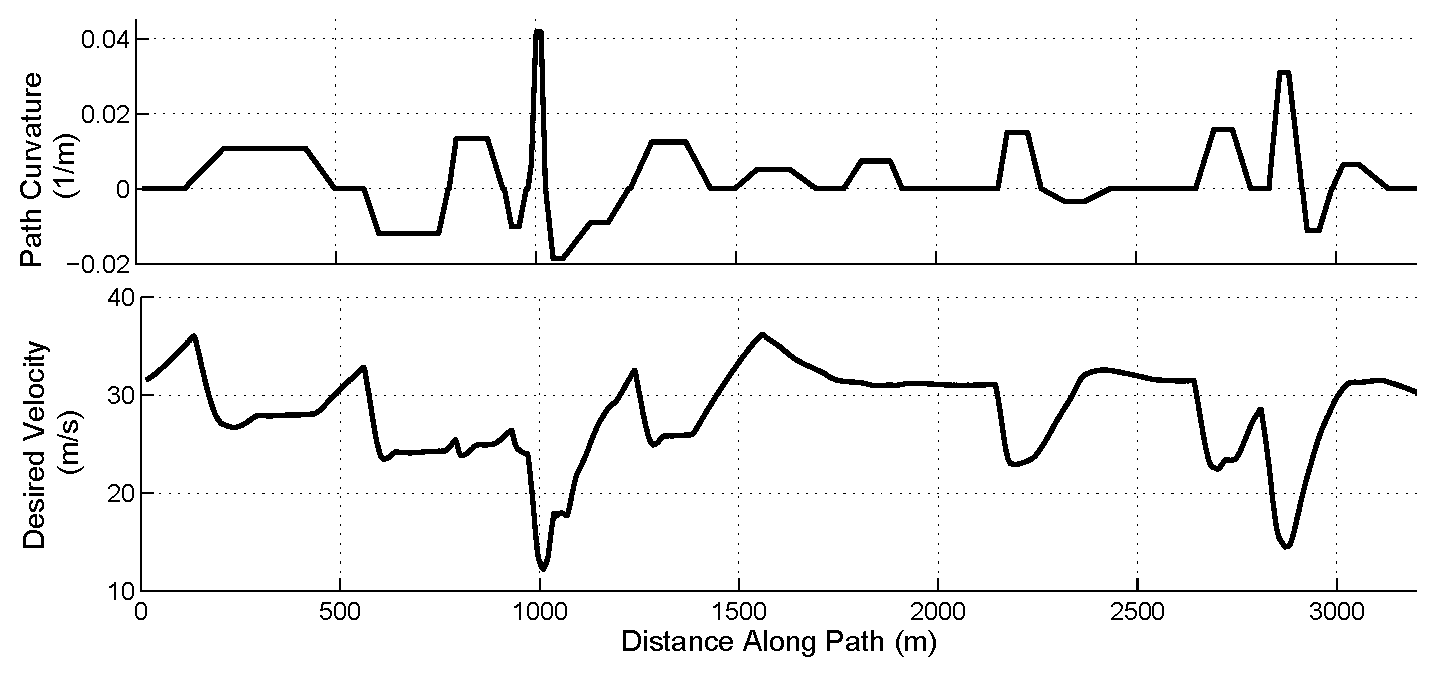
\includegraphics[width=\fullwidth]{traj.eps}
\caption{Curvature and velocity profile inputs for steering controller as a function of distance along racing line.}
\label{fig:traj}
\end{figure}


\begin{figure}[h]
\centering
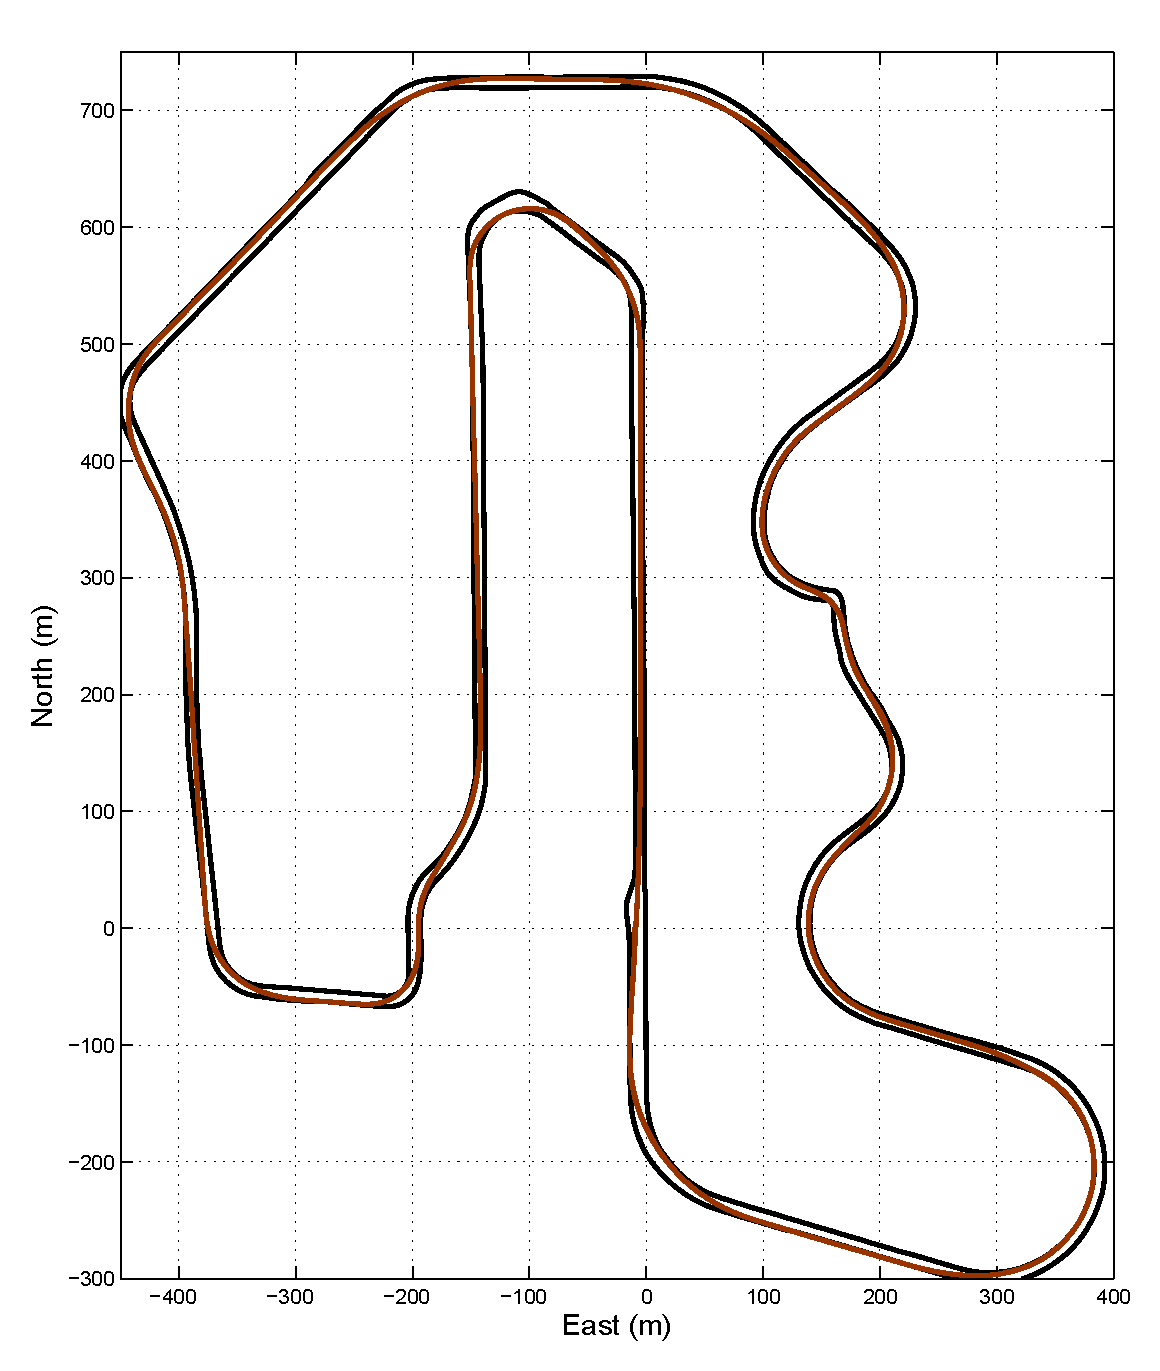
\includegraphics[width=\fullwidth]{racingLine.eps}
\caption{Desired path for steering controller to follow.}
\label{fig:thPic}
\end{figure}

\section{Experimental Testing of Sideslip Feedback \newline Controller}

The steering feedback controller with sideslip-path tangency presented in Section \ref{sec:betafb} offers very low path tracking error, but at the
expense of reduced stability margins. To test this controller safely at the limits of handling, experimental data was collected on a
constant radius turn in an open parking lot at two constant speeds. The results of this test are shown in Fig.~\ref{fig:wipeout}. As a baseline, the
feedback controller with sideslip (\ref{eqn:vveq}) from Section \ref{sec:betafb} is compared to the original lookahead feedback controller (\ref{eqn:lookahead}). 
The feedforward steering based on the nonlinear handling diagram (\ref{eqn:steadyffw}) is used in both cases. 
For the case where the speed is 10 m/s, the resulting steady-state acceleration is 7 $\mathrm{m/s^2}$, and both steering controllers maintain stability of the vehicle. 
In addition, incorporating sideslip-path tangency into the feedback control law results in significantly lower path tracking errors compared to the baseline
lookahead feedback controller.

 However, when the speed is increased to 13 m/s, the resulting steady-state lateral acceleration is 9 $\mathrm{m/s^2}$,
and the sideslip feedback controller becomes unstable, causing the vehicle to spin out spin, as demonstrated by the plots of yaw rate and sideslip. For the same conditions,
the baseline lookahead controller remains stable. The issue with the sideslip feedback controller is shown in the plot of vehicle sideslip and heading
error. As the vehicle heading error decreases and becomes unstable around $s = $ 170 m, the feedback controller does not intervene because the
 vehicle's velocity vector remains tangent to the path (i.e. $\Delta\Psi + \beta =$ 0). A counter steering action is finally provided at $s = $ 190 m, but at this point the vehicle
has already spun out.

\begin{figure}
\centering
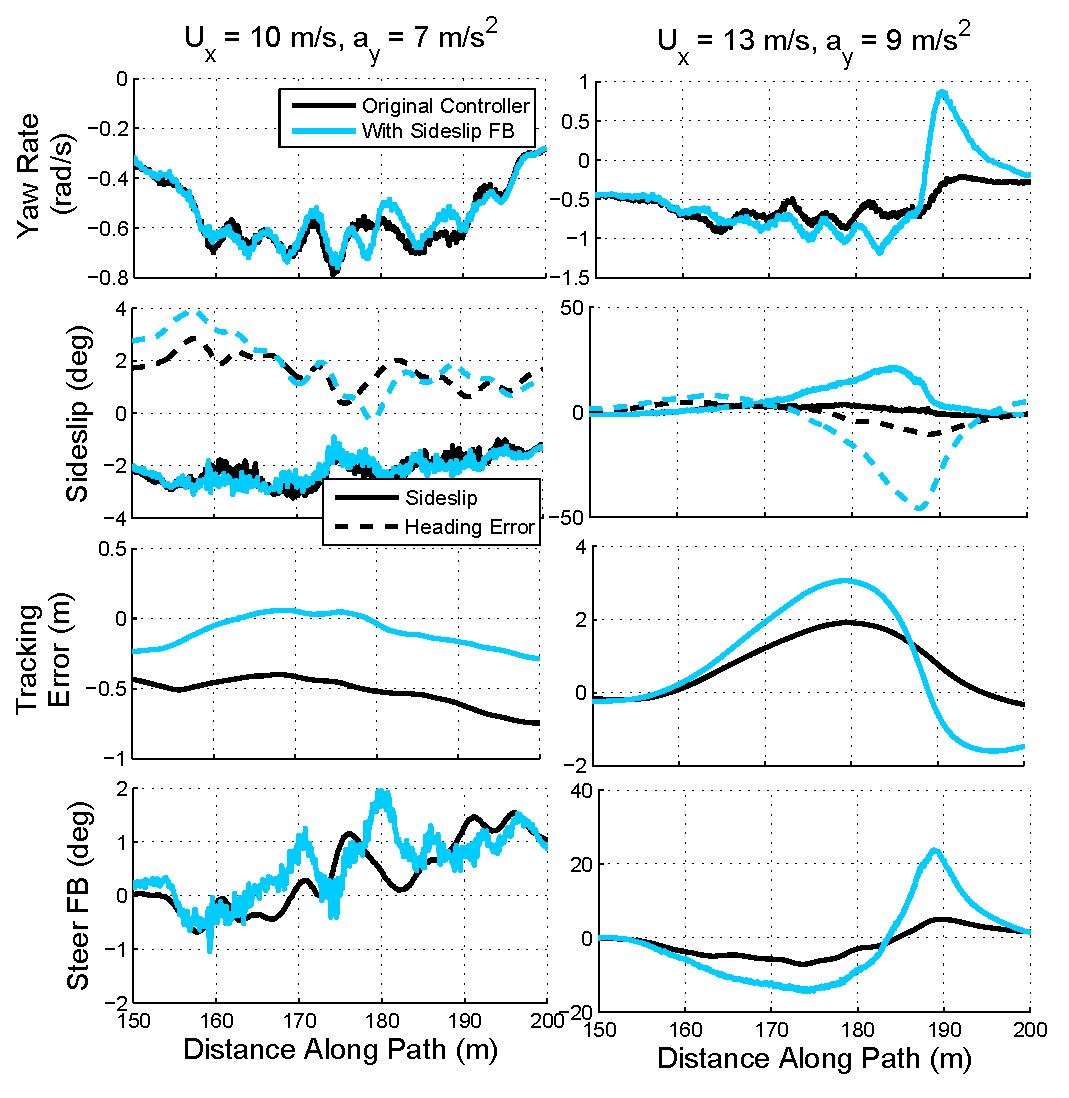
\includegraphics[width=\fullwidth]{wipeout.eps}
\caption[Parking lot test for constant radius turning at 10 m/s and 13 m/s.]{Parking lot test for constant radius turning at 10 m/s and 13 m/s. Resulting steady-state accelerations are 7 $\mathrm{m/s^2}$ and 9
$\mathrm{m/s^2}$. Steering feedback with sideslip is compared to original lookahead steering controller.}
\label{fig:wipeout}
\end{figure}


\section{Experimental Data from Racetrack}

Fig.~\ref{fig:betaComparison} shows experimental data taken over a 3 km subset of the entire racetrack,
excluding portions of the course where there is little vehicle cornering. The experimental data is plotted for two separate steering
controllers. The first controller is the baseline controller described in \S \ref{sec:controllerC2}, with the
steering feedback provided by the lookahead system and the feedforward steering given by the steady-state handling diagram. The second controller uses the same lookahead feedback, but incorporates the steady-state sideslip
behavior into the feedforward steering to align the vehicle's velocity vector with the path heading (\S \ref{sec:goodFFW}).
Note that the controller where real-time sideslip was incorporated into the steering feedback (\S \ref{sec:betafb}) was not tested, as there is a high likelihood
of vehicle instability near the limits of handling given the results from the previous parking lot test. The same longitudinal controller is used for both cases in order to
 brake into the entry of turns and accelerate out of turn exits. For this lap, the peak longitudinal deceleration is -8 $\mathrm{m/s^2}$ and
 peak lateral acceleration is 8 $\mathrm{m/s^2}$.
 
\begin{figure}[h!]
\centering
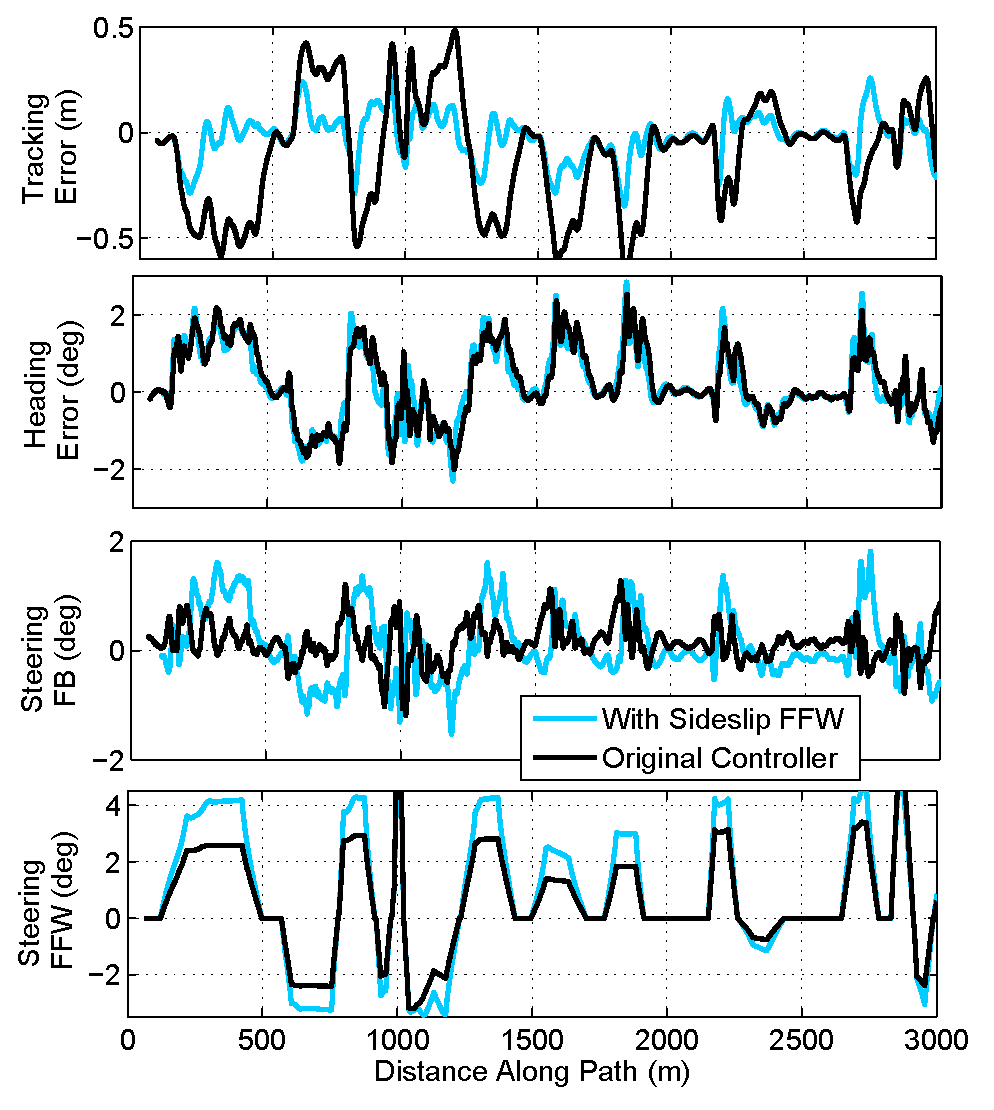
\includegraphics[width=\fullwidth]{betaCompensation.eps}
\caption{Experimental data with combined acceleration magnitude 8 $\mathrm{m/s^2}$ over a 3 km stretch of Thunderhill Raceway Park. Results are
shown for both the baseline FB-FFW controller and the modified controller with sideslip tracking in the feedforward loop.}
\label{fig:betaComparison}
\end{figure}

The results in Fig.~\ref{fig:betaComparison} show that lateral path deviation $e$ is reduced when incorporating 
steady-state sideslip in the feedforward control law. This confirms the expected results from the analysis performed in \S \ref{sec:predSS}
and \S \ref{sec:goodFFW}. Note that while the lateral path deviation is smaller, the levels of vehicle heading error $\Delta\Psi$ remain roughly the
same. This matches the predicted result in Fig.~\ref{fig:linError2}. The steering controller will align the vehicle's
velocity vector with the path, not the vehicle's heading, and due to a vehicle's tendency to develop a steady-state sideslip angle,
 a non-zero heading error $\Delta\Psi$ is in general necessary for zero steady-state lateral path deviation,
 as shown by the schematic in Fig.~\ref{fig:SSerror}.

 For a better comparison of the lateral path deviation, Fig.~\ref{fig:errhist} shows histograms of the lateral tracking
error $e$ for both controllers at three levels of peak lateral acceleration. The baseline controller keeps the vehicle within 0.5 meters
 on either side of the desired path, with a large
amount of variation in the resulting histogram. An interesting observation is that the 
histogram is not symmetric. In general, the raceway has more left turns than right turns, and as Fig.~\ref{fig:linError} indicates, at
high speeds the baseline controller will track toward the outside of the turn. This tendency is manifested experimentally in the asymmetric nature
of the histograms. The histograms for the improved controller show a much tighter distribution on the lateral path tracking 
error. The path tracking error generally remains within 10-15 cm on either side of the lane boundary and contains less of a bias towards tracking
on the outside of turns.  
 
\begin{figure}
\centering
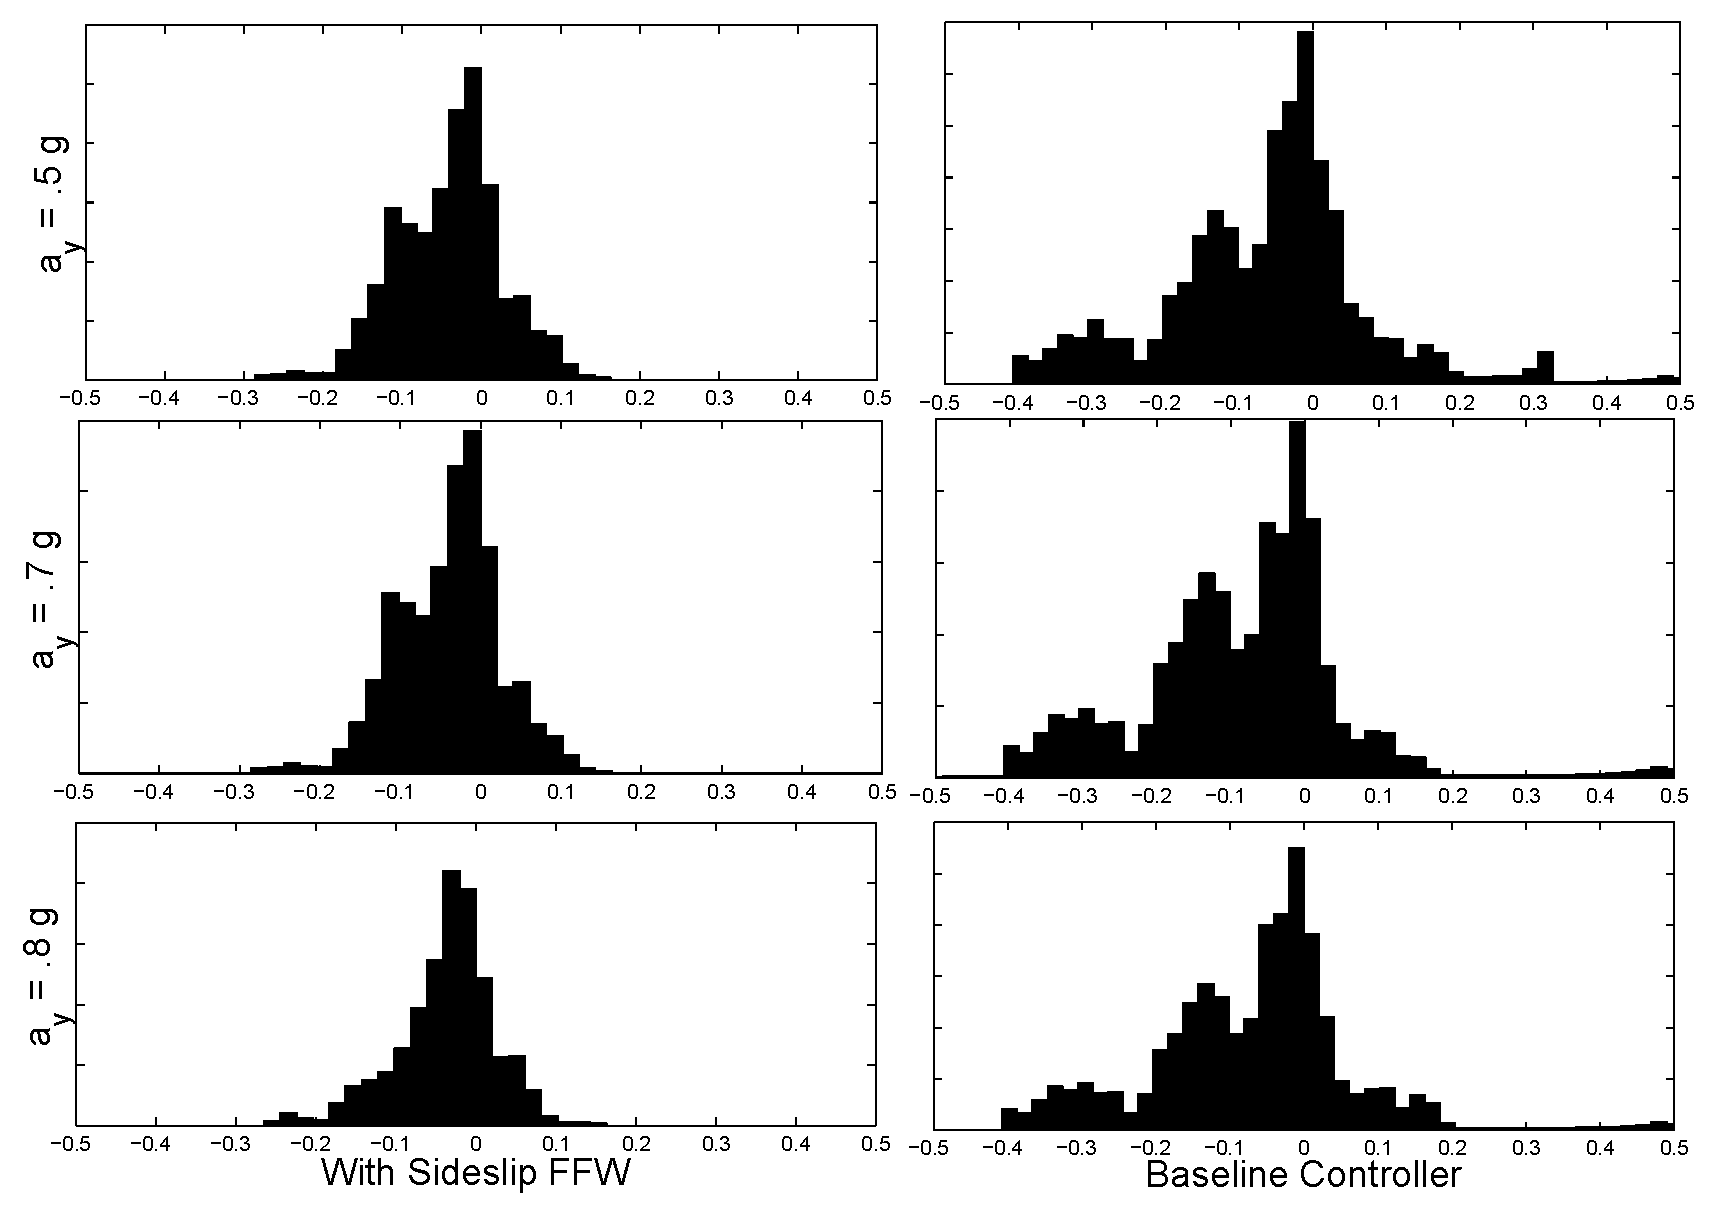
\includegraphics[width=\fullwidth]{errhist.eps}
\caption[Histogram of path tracking error for six laps around the track.]{Histogram of path tracking error for six laps around the track. Left column represents performance of controller
with feedforward sideslip tracking, and right column is baseline controller with feedforward from
the steady-state handling diagram. Path tracking error is in meters.}
\label{fig:errhist}
\end{figure}

As the lateral acceleration increases beyond 0.8 g and the vehicle approaches the handling limits, the steering controller
remains stable and well-damped, although the tracking performance begins to degrade. Fig.~\ref{fig:atTheLimits} shows experimental
data for a lap around Thunderhill Raceway park with peak lateral and longitudinal accelerations of 0.95 g. At several points along the
track, the tracking error increases above 0.5 m, significantly higher than the levels of path deviation seen at 0.8 g of vehicle acceleration.
The reasons for this are three-fold. 

\begin{figure}
\centering
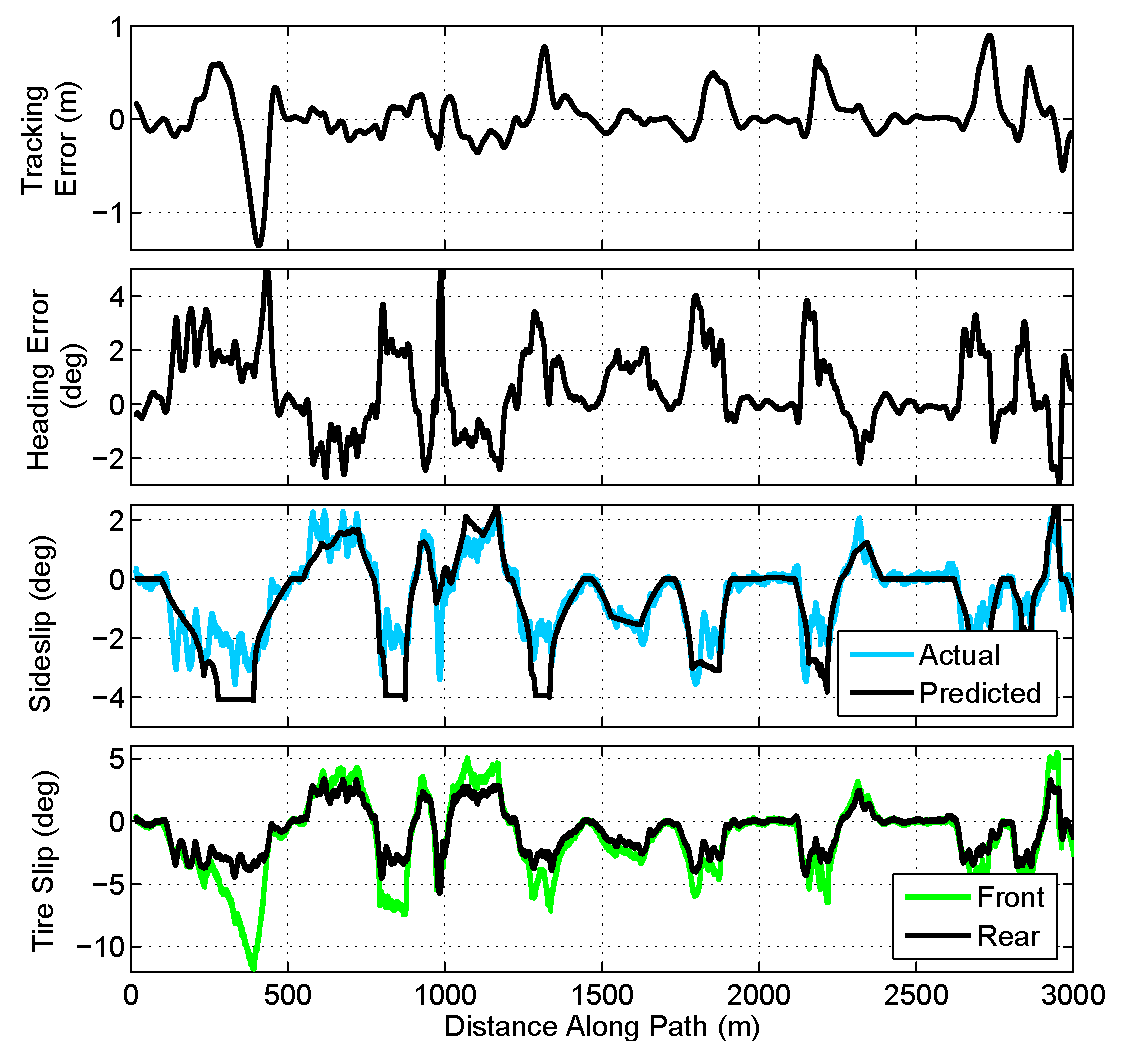
\includegraphics[width=\fullwidth]{atTheLimits.eps}
\caption{Experimental data with combined acceleration magnitude 9.5 $\mathrm{m/s^2}$ over a 3 km stretch of Thunderhill Raceway Park.}
\label{fig:atTheLimits}
\end{figure}

First, the sharp drop in front tire slip from $s$ = 300 to 400 meters indicates that the 
 lateral force demand for the front tires has exceeded the available friction at that region of the track. As a result, the vehicle
 understeers heavily and tracks well to the outside of the left-hand turn, resulting in a large negative tracking error.
At this point, there is nothing the steering controller can do to bring the vehicle back to the desired path, and the vehicle must alter its
desired trajectory to become less aggressive, either by slowing down or reducing the turn curvature. Second, the steady-state feedforward controller requires an accurate estimate of the vehicle parameters in order to estimate
the steady-state sideslip in (\ref{eqn:betass}). From $s$ = 700-800, 1300-1400, 1800-1900, and 2200-2300 meters along the track, there are observable
discrepancies between the predicted feedforward sideslip and the actual vehicle sideslip, as measured by the GPS-INS. This plant-model mismatch results in significant path tracking errors at those portions of the racing circuit. Finally, the feedforward
model in (\ref{eqn:betass}) assumes steady-state conditions. As the vehicle approaches the limits of handling, transient vehicle
dynamics can result in larger path deviations as well.

The lap-to-lap learning algorithms presented in Chapter 4 focus on reducing the latter two sources of
 error by gradually learning a better feedforward model of the
vehicle dynamics over time. For situations where a vehicle repeats a 
given trajectory multiple times, iterative learning control (ILC)
is a promising technique for refining the feedforward input to improve
 the reference tracking performance of the controller. Additionally, online estimation
approaches can also be used to gradually improve knowledge 
of difficult-to-measure parameters such as friction and vehicle cornering
stiffness.

% %=======================================================================
\section{Conclusion}

This chapter describes the design of a feedback-feedforward controller capable of path tracking at the limits of handling. Desirable
 path tracking behavior occurs when the vehicle sideslip is aligned
with the desired path heading. However, directly incorporating this behavior into a feedback steering control law results in 
a closed-loop controller with poor stability margins. 
A better approach for combined path tracking and stability is to align the steady-state vehicle sideslip 
with the desired path heading through the feedforward steering command. 

The benefit of the presented work is a controller design that provides low path tracking error over a large
range of vehicle lateral accelerations. More importantly, the lateral path tracking improvement is achieved without
sacrificing the robust stability properties of the lookahead steering feedback. Results from
a histogram analysis quantitatively indicate that the improved feedforward command reduces lateral path deviation from the baseline
controller by more than fifty percent. One potential drawback is that this feedforward approach is sensitive to vehicle model uncertainty, especially at the physical
limits of handling where transient dynamics become prevalent. Chapter 4 will present iterative learning control
algorithms to improve the feedforward vehicle model and eliminate undesirable transient dynamics. 

 \textit{Note: This chapter reuses material previously published by the author in \cite{kapania}.}
% \begin{enumerate}
% \item \textit{Kapania and Gerdes. Design of a feedback-feedforward steering controller for accurate path tracking and stability at the limits of handling. Vehicle System Dynamics 2015 \cite{kapaniaVSD}} 
% \item \textit{Kapania and Gerdes. An Autonomous Lanekeeping System for Vehicle Path Tracking and Stability at the Limits of Handling. AVEC 2014 \cite{kapania}.}
% \end{enumerate}

%\\
% enable cross referencing between chapters
\chapter{Fast Generation Path Planning}
\label{chapter3}

 Chapter 2 presented a steering controller capable of driving an aggressive trajectory from
 a high level trajectory planner. Since the steering controller only requires the curvature and 
 velocity profile output, the details of the trajectory planner were not considered for the controller design.
 However, for the purpose of race car driving, the trajectory planning phase is just as important as the real-time path following. This
 chapter therefore provides a novel approach for planning the trajectory of an automated race vehicle. Because of the
 focus on racing, the primary consideration of the trajectory generation algorithm will be minimizing the vehicle's lap time.
 %\footnote{Future modifications of the presented 
 %algorithm to passenger safety applications will be discussed in Chapter 6.}
 
 The problem of calculating the minimum lap time trajectory for a given vehicle and race track has been studied over the last several decades
in the control, optimization, and vehicle dynamics communities.  Early research by Hendrikx et al. \cite{hendrikx} in 1996 used 
 Pontryagin's minimum principle to derive coupled differential equations to solve for the minimum-time trajectory
for a vehicle lane change maneuver. A geometric analysis was also presented by Gordon et al., where vector fields representing the vehicle's velocity
were generated at every location on the road with the friction circle used as a constraint on the field's gradient \cite{gordon}. In 2000, Casanova \cite{casanova} published a method to optimize both the path and speed profile
for a fully nonlinear vehicle model using nonlinear programming (NLP). Kelly \cite{kelly} further extended the results from Casanova by considering
the physical effect of tire thermodynamics and applying more robust NLP solution methods such as Feasible Sequential Quadratic Programming. More recently,
Perantoni and Limebeer \cite{perantoni} showed that the computational expense could be significantly reduced by 
applying curvilinear track coordinates, non-stiff vehicle dynamics, and the use of smooth computer-generated
analytic derivatives. 

The primary focus of these NLP solutions was developing a simulation tool for Formula One race teams to analyze the lap time effects of 
subtle race car modifications. As a result, experimental validation was not considered, and high computation times were not a major issue. However, the development 
of autonomous vehicle technology has led to research on optimal path
 planning algorithms that can be validated on driverless cars. Theodosis and Gerdes published a gradient descent approach 
 for determining time-optimal racing lines, with the racing line constrained to be composed of a fixed number of clothoid segments that are amenable
for autonomous driving \cite{theodosis}\footnote{The curvature and speed profile used for the controller validation in Chapter 2 came from the racing trajectory generated
 by Theodosis and Gerdes.}. When driven autonomously
  using a closed-loop trajectory following controller \cite{kapania}\cite{mickcop}, the resulting lap times were within one second of lap times from
  a professional race car driver. However, the gradient descent method, like other nonlinear programming techniques, took several hours of computation time to complete on a standard
  desktop computer. 
  
  Given the computational expense  of performing nonlinear optimization, there has recently been an effort to find
  approximate methods that provide fast lap times.
 Timings and Cole \cite{timings} formulated the minimum lap time problem into a model predictive control (MPC) problem
 by linearizing the nonlinear vehicle
 dynamics at every time step and approximating the minimum-time objective by maximizing distance traveled along the path centerline.
  The resulting racing line
 for a 90 degree turn was simulated next to an NLP solution. Liniger et al. \cite{morari} presented both a receding horizon and
 model predictive contour control approach for real-time autonomous racing. Like \cite{timings}, the guiding principle for both controllers
 was locally maximizing distance traveled along the centerline. Gerdts et al. \cite{gerdts} proposed a 
 similar receding horizon approach, where distance along a reference path was maximized over a series of locally optimal optimization
 problems that were combined with continuity boundary conditions. One potential drawback of the model predictive control approach is that an optimization
 problem must be reformulated and solved at every time step, which can still be computationally expensive. For example, Timings and Cole reported a computation time of 900 milliseconds
 per 20 millisecond simulation step with the CPLEX quadratic program solver on a desktop PC. By shortening the lookahead horizon from 500 time steps to 50 time steps and approximating
 the function to calculate distance traveled, Liniger et al. was able to demonstrate real-time autonomous racing on 1:43 scale RC cars \cite{morari}.  
 
  In summary, due to the primary objective of minimizing lap time while staying on the race track, constrained optimization
  is frequently used for planning a minimum-time trajectory. The most common method 
  is nonlinear programming, which provides low lap-time trajectories, but at the expense of 
  high computation times. The complex nature of the minimum-time vehicle optimization problem is two-fold. First, two sets of vehicle inputs, longitudinal and
 lateral, must be determined. Unfortunately, the lateral and longitudinal dynamics become highly coupled and nonlinear at the limits of handling. Second, directly minimizing
 lap time requires minimizing a non-convex cost function (\S \ref{sec:UPDATE}). Not only are non-convex optimization problems more expensive to solve than their convex counterparts, but
 solution techniques are also only guaranteed to converge to a local minima. While computation time is not an issue for
 simulation tools, with the rapid progress in autonomous vehicle technology, there are significant benefits
 to a trajectory generation algorithm that can rapidly approximate the fastest racing trajectory for at least
 the next several turns of the race track (see \S \ref{ch1FGbenefits}). 
 
 This chapter therefore presents an experimentally validated algorithm that bypasses the complexity of minimum-time vehicle
 optimization in order to generate racing trajectories with low computational expense. To avoid the issue of coupled control inputs, the combined
 lateral/longitudinal optimal control problem is replaced by two sequential sub-problems that are solved iteratively. In the first
 sub-problem, the minimum-time longitudinal speed inputs are computed given
 a fixed vehicle path. In the second sub-problem, the vehicle path is updated given the fixed speed commands. To avoid minimizing
the non-convex lap time cost function, the vehicle path is updated by solving a convex minimum curvature heuristic. The concept of solving a coupled, 
non-convex optimization via sequential approximations is not new, and the proposed approach is inspired by the methodology used in sequential convex
programming (SCP) and the expectation/maximization (EM) algorithm \cite{diehl}\cite{tibstibs}.\footnote{Sequential convex programming attempts to solve a nonconvex optimization problem by iteratively solving a convex approximation over a trust region that is modified after every iteration. Expectation/Maximization
determines maximum likelihood estimates in statistical models with unobserved variables by repeatedly alternating between an expectation step and a maximization step. } 
The biggest potential drawback of these approaches is that the guarantee of 
convergence to a globally optimal solution is lost, and the proposed method is therefore as sensitive to initial conditions as any nonlinear optimization.    
 
 The following section presents a mathematical framework for the trajectory generation
 problem and provides a linearized five-state model for the planar dynamics of a racecar following speed and steering inputs on a fixed path. 
 This model is identical to the model presented in Chapter 2, where the lateral vehicle dynamics are explicitly
 modeled but the longitudinal speed $U_x$ is treated as a time-varying parameter. 
 Section \ref{sec:VP} describes the method of finding the minimum-time speed inputs given a fixed path. 
 While this sub-problem has been recently solved using convex optimization \cite{lipp}, a forward-backward
 integration scheme based on prior work \cite{subosits} is used instead.  Section \ref{sec:UPDATE} describes
 a method for updating the racing path given the fixed speed inputs using convex optimization, 
 where the curvature norm  of the driven path is explicitly minimized. 
 
 The complete algorithm is outlined in \S \ref{sec:IMPLEMENT}, and a trajectory is generated for the Thunderhill Raceway circuit
 from Chapter 2. This trajectory is compared with a trajectory recorded from a professional human driver and the gradient descent
 trajectory from Theodosis \cite{theodosis}. In \S \ref{sec:EXP}, the generated racing trajectory is validated experimentally in
 the autonomous Audi TTS testbed using the path-following controller from Chapter 2. The resulting lap time compares well with the lap times
 recorded for the gradient descent trajectory and the human driver. However, there are particular sections of the track where minimizing the driven
 curvature does not provide a fast trajectory. Section \ref{sec:ADDMINDIST} therefore proposes a modified cost function for the path update
 step that also incorporates the benefit of reducing the length of the racing line. Section \ref{sec:DISCUSSION} concludes by discussing 
 future implementation of the algorithm in a real-time path planner.  

\section{Path Description and Vehicle Model}
\label{sec:PATH}
Figure~\ref{fig:worldInfo} describes the parameterization of the reference path that the vehicle will follow. The
reference path and road boundaries are most intuitively described in Fig.~\ref{fig:worldInfo}(a) via Cartesian East-North coordinates. However, for the purposes of quickly generating
a racing trajectory, it is more convenient to parameterize the reference path as a curvature profile $\kappa$ that is a function of distance along the path $s$ (Fig.~\ref{fig:worldInfo}(c)). Additionally, it is 
convenient to store the road boundary information as two functions $w_\mathrm{in}(s)$ and $w_\mathrm{out}(s)$, which correspond to the lateral distance from the path at $s$
 to the inside and outside road boundaries, respectively (Fig.~\ref{fig:worldInfo}(b)). This maximum lateral distance representation will be useful when constraining the generated racing path to lie within the road 
 boundaries. The transformation from curvilinear $s$, $\kappa$ coordinates to 
Cartesian coordinates $E$, $N$ are given by the Fresnel integrals:
\begin{subequations}
\label{eq:fresnel}
\begin{align}
	E(s) &= \int_0^s  -\sin(\Psi_\mathrm{r}(z)) dz \\
	N(s) &= \int_0^s   \cos(\Psi_\mathrm{r}(z)) dz \\
	\Psi_\mathrm{r}(s) &= \int_0^s \kappa(z) dz \label{eq:balls}
\end{align}
\end{subequations}
where $\Psi_\mathrm{r}(s)$ is the heading angle of the reference path and $z$ is a dummy variable. 

With the reference path defined in terms of $s$ and $\kappa$, the 
next step is to define the dynamic model of the vehicle. For the purposes of trajectory generation, we assume the vehicle dynamics are given 
by the same planar bicycle model presented in Chapter 2, with 
yaw rate $r$ and sideslip $\beta$ states describing the lateral dynamics. 
Additionally, the vehicle's offset from
the reference path are again given by the path lateral deviation state $e$ and path heading error state $\Delta\Psi$. 
Linearized equations of motion for all four states are given by (\ref{eq:bm}). Recall that that while 
the vehicle longitudinal dynamics are not explicitly modeled, the bicycle model does allow for time-varying values of $U_x$. 
This is a reasonable approximation because the vehicle model will be used for the lateral path update step, 
whereas the longitudinal dynamics will be treated separately in the velocity profile generation step. 

\begin{figure}
\centering
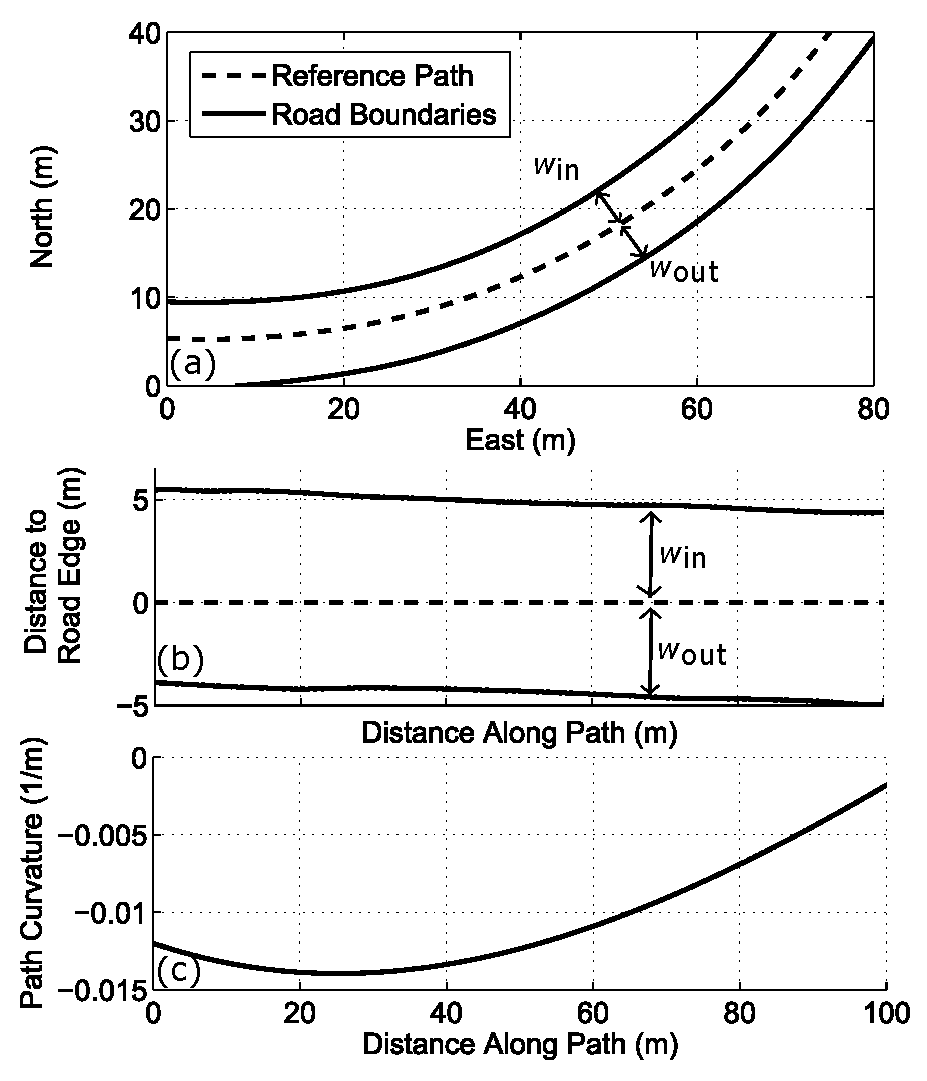
\includegraphics[width=.85\fullwidth]{worldInfo.eps}
\caption[View of sample reference path and road boundaries]{(a) View of a sample reference path and road boundaries, plotted in the East-North Cartesian frame (b) Lateral distance from path to inside road edge (positive) and outside road edge (negative) as a function
of distance along path. (c) Curvature as a function of distance along path.}
\label{fig:worldInfo}
\end{figure}

\section{Velocity Profile Generation Given Fixed \newline Reference Path}
\label{sec:VP}

Given a fixed reference path described by $s$ and $\kappa$, the first algorithm step is to find the 
minimum-time speed profile the vehicle can achieve
without exceeding the available friction. 
While finding the minimum-time speed profile for a fixed path was recently solved as a convex problem by Lipp and Boyd \cite{lipp}, the
 algorithm presented in this chapter directly uses the ``three-pass" approach described by 
Subosits and Gerdes \cite{subosits}, and originally inspired by work from Velenis and Tsiotras \cite{velenis}
and Griffiths \cite{griffiths}. 
Given the lumped front and rear tires from the bicycle model, the available longitudinal
 and lateral forces $F_\mathrm{x}$ and $F_\mathrm{y}$ at each wheel are constrained by the friction circle: 
\begin{subequations}
\label{eq:tireforce}
\begin{align}
	F^2_\mathrm{xf} + F_\mathrm{yf}^2 &\leq (\mu F_\mathrm{zf})^2\\
	F^2_\mathrm{xr} + F_\mathrm{yr}^2 &\leq (\mu F_\mathrm{zr})^2
\end{align}
\end{subequations}
where $\mu$ is the tire-road friction coefficient and $F_\mathrm{z}$ is the available normal force. The first pass of the speed profile generation finds the maximum permissible
 vehicle speed given zero longitudinal force. For the simplified case where weight transfer and topography effects are neglected, this is given by:
\begin{equation}
\label{eq:steadystate}
	U_x(s) = \sqrt{\frac{\mu g}{|\kappa(s)|}}
\end{equation}
where the result in (\ref{eq:steadystate}) is  obtained by setting $F_\mathrm{yf} = \frac{mb}{a+b}U_x^2\kappa$ and $F_\mathrm{zf} = \frac{mgb}{a+b}$.
 The results of this first pass for the sample curvature profile in Fig.~\ref{fig:VPgen}(a) are shown in Fig.~\ref{fig:VPgen}(b).
 The next step is a forward 
integration step, where the velocity of a given point is determined by the velocity of the previous point and the available longitudinal force $F_{x,\mathrm{max}}$ for acceleration.
This available longitudinal force is calculated in \cite{subosits} by accounting for the vehicle engine force limit and the lateral force demand on all tires due to the road curvature:
\begin{equation}
\label{eq:forwardint}
	U_x(s+\Delta s) =\sqrt{U^2_x(s)+\mathrm{2}\frac{F_{x,\mathrm{accel,max}}}{m}\Delta s}
\end{equation}
A key point of the forward integration step is that at every point, the value of $U_x(s)$ is compared to the corresponding value from (\ref{eq:steadystate}), and
the minimum value is taken. The result is shown graphically in Fig.~\ref{fig:VPgen}(c). Finally, the backward integration step occurs, where the available
longitudinal force for deceleration is again constrained by the lateral force demand on all tires:
\begin{equation}
\label{eq:backwardsint}
	U_x(s-\Delta s) = \sqrt{U^2_x(s)-\mathrm{2}\frac{F_{x,\mathrm{decel,max}}}{m}\Delta s}
\end{equation}
The value of $U_x(s)$ is then compared to the corresponding value from (\ref{eq:forwardint}) for each point along the path, and the minimum
value is chosen, resulting in the final velocity profile shown by the solid line in Fig.~\ref{fig:VPgen}(d). While treatment of three-dimensional road 
effects are not described in this chapter, the method described in \cite{subosits} and
used for the experimental data collection determines the normal and lateral tire forces $F_\mathrm{z}$ and $F_\mathrm{y}$ at each point along the path 
by accounting for weight transfer and bank/grade of the road surface. 

 \begin{figure}
\centering
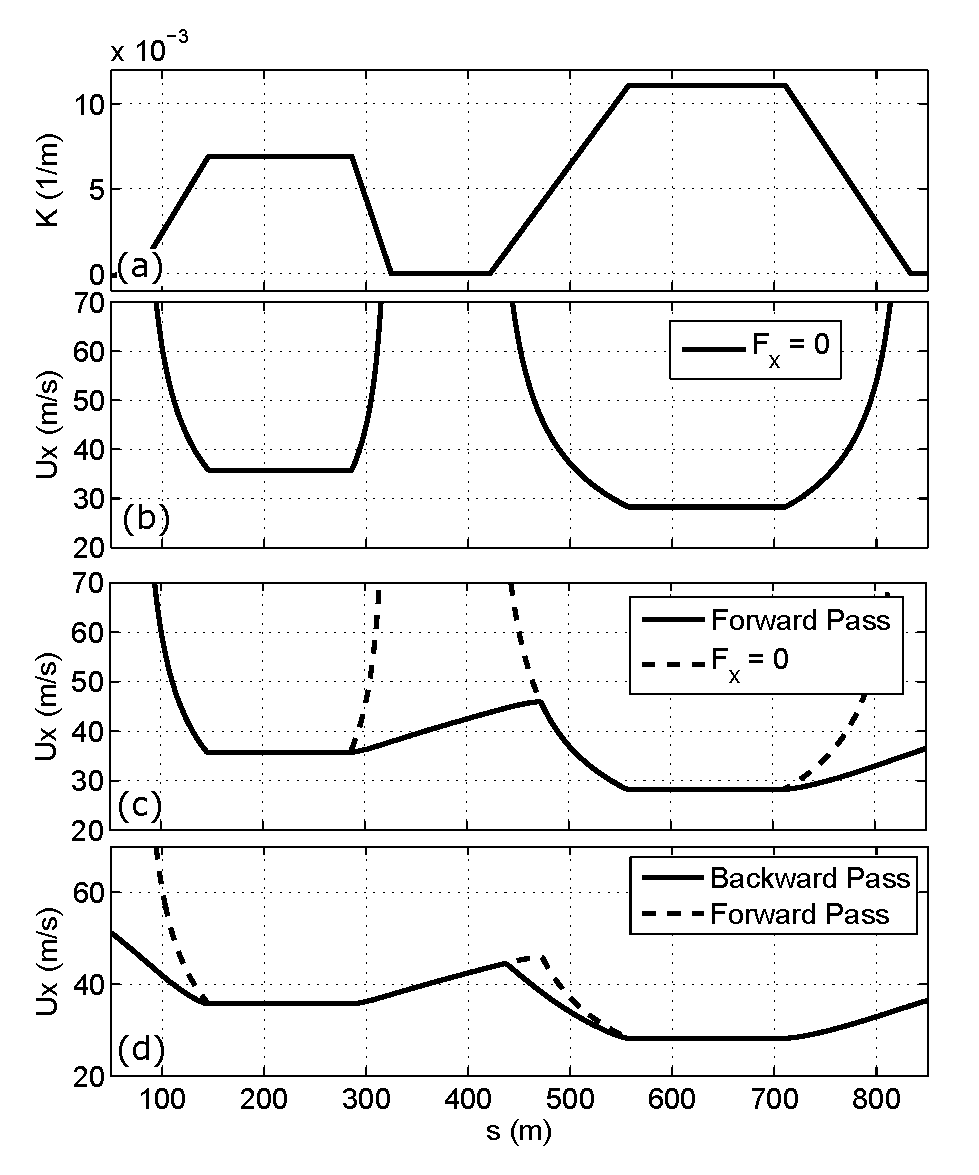
\includegraphics[width=\fullwidth]{vpgen.eps}
\caption[Velocity profile generation illustration]{(a) Sample curvature profile. (b) Velocity profile given zero longitudinal force. (c) Velocity profile after forward pass. (d) Final velocity profile after backward pass. }
\label{fig:VPgen}
\end{figure}

\section{Updating Path Given Fixed Velocity Profile}
\label{sec:UPDATE}
\subsection{Overall Approach and Minimum Curvature Heuristic}
The second step of the trajectory generation algorithm takes the original reference path $\kappa(s)$ and corresponding velocity profile $U_x(s)$
as inputs, and modifies the reference path to obtain a new, ideally faster, racing line. Sharp \cite{sharp} suggests a general approach for modifying 
an initial path to obtain a faster lap time by taking the original path and velocity profile and incrementing the speed uniformly
by a small, constant ``learning rate." An optimization problem is then solved to find a new reference path and control inputs that allow the vehicle to
drive at the higher speeds without driving off the road. If a crash is detected, the speed inputs are locally reduced around the crash site and the process is repeated.

However, one challenge with this approach is that it can take several hundred iterations of locally modifying the vehicle speed profile, detecting crashes, and 
 modifying the reference path to converge to a fast lap time. An alternative approach is to modify the reference path in one step by solving a single 
 optimization problem. The lap time $t$ for a given racing line is provided by the following equation: 
 
 \begin{equation}
t = \int_0^l\frac{ds}{U_x(s)}
\label{integrateEq}
\end{equation}
 
 Equation (\ref{integrateEq}) implies that minimizing the vehicle lap time requires simultaneously minimizing the total path length $l$ while maximizing
 the vehicle's longitudinal velocity $U_x$. These are typically competing objectives, as lower curvature (i.e. higher radius) paths can result in longer path lengths but higher
 vehicle speeds when the lateral force capability of the tires is reached, as shown in (\ref{eq:steadystate}). Since (\ref{integrateEq}) is a nonconvex cost function in the
 optimization variables, time-intensive nonlinear programming is required to manage this curvature/distance trade-off and explicitly minimize the lap time. 
 
 The proposed approach is therefore to simplify the cost function by only minimizing the norm of the vehicle's driven curvature
 $\kappa(s)$ at each path modification step. Path curvature can be easily formulated as a convex function with respect to the vehicle state vector $x$, 
 enabling the path modification step to be easily solved by leveraging the computational speed of convex optimization. 
 
 However, minimizing curvature is not the same as minimizing lap time and provides
 no guarantee of finding the time-optimal solution. The proposed cost function relies on the hypothesis that a path with minimum curvature is a good approximation for
 the minimum-time racing line. Lowering the curvature of the racing line is more important than minimizing
 path length for most race courses, as the relatively narrow track width provides limited room to shorten the overall path length. Simulated and experimental results
 in \S \ref{sec:IMPLEMENT} and  \S \ref{sec:EXP} will validate this hypothesis by showing similar lap time performance when compared to
 a gradient descent method that directly minimizes lap time. However, a particular section of the race track where the minimum curvature
 solution shows poor performance will be discussed as well, and improved upon in \S \ref{sec:ADDMINDIST}. 

\subsection{Convex Problem Formulation}

Formulating the path update step as a convex optimization problem requires an affine, discretized form of the
bicycle model presented earlier. The equations of motion in (\ref{eq:bm}) are already linearized, but
 the front and rear lateral tire forces become saturated as the vehicle drives near the limits of tire adhesion. 
The well-known brush tire model \cite{Pacejka2012}, also presented in Chapter 2, captures the effect of tire saturation:
\begin{eqnarray}
\label{eq:fiala}
	F_\mathrm{y\diamond}&=&\begin{cases} -C_{\diamond}\tan\alpha_\diamond + \frac{C_\diamond^2}{3\mu F_\mathrm{z\diamond}} |\tan\alpha_\diamond| \tan\alpha_\diamond \\ \hspace{10mm}- \frac{C_\diamond^3}{27\mu^2F_\mathrm{z\diamond}^2}\tan^3\alpha_\diamond,
\hspace{8mm}  |\alpha_\diamond| < \arctan{\left(\frac{3\mu F_\mathrm{z\diamond}}{C_\diamond}\right)} \\ \\ -\mu F_\mathrm{z\diamond}\text{sgn} \ \alpha_\diamond, \hspace{36mm} \mathrm{otherwise} \end{cases}
\end{eqnarray}
where the symbol $\diamond \in [\mathrm{f},\mathrm{r}]$ denotes the lumped front or rear tire, and $C_\diamond$ is the corresponding tire cornering stiffness. 

\newpage
The linearized tire slip angles $\alpha_\mathrm{f}$ and $\alpha_\mathrm{r}$ are functions of the vehicle lateral states and the steer angle
input, $\delta$:
\begin{subequations}
\begin{align}
	\alpha_\mathrm{f} &= \beta + \frac{ar}{U_x} - \delta\\
	\alpha_\mathrm{r} &= \beta - \frac{br}{U_x}
\end{align}
\end{subequations}
The brush tire model in (\ref{eq:fiala}) can be linearized at every point along the reference path assuming steady state cornering conditions:
\begin{subequations}
\begin{align}
	F_\mathrm{y\diamond} &= \tilde{F}_\mathrm{y\diamond} - \tilde{C}_\diamond(\alpha_\diamond - \tilde{\alpha}_\diamond) \\
	\tilde{F}_\mathrm{y\diamond} &= \frac{F_\mathrm{z\diamond}}{g} U_x^2\kappa
\label{eqn:ftil}
\end{align}
\end{subequations}
with parameters $\tilde{F}_\mathrm{y}$, $\tilde{\alpha}$ and $\tilde{C}$ shown in Fig.~\ref{fig:fiala}. 

\begin{figure}[h]
\centering
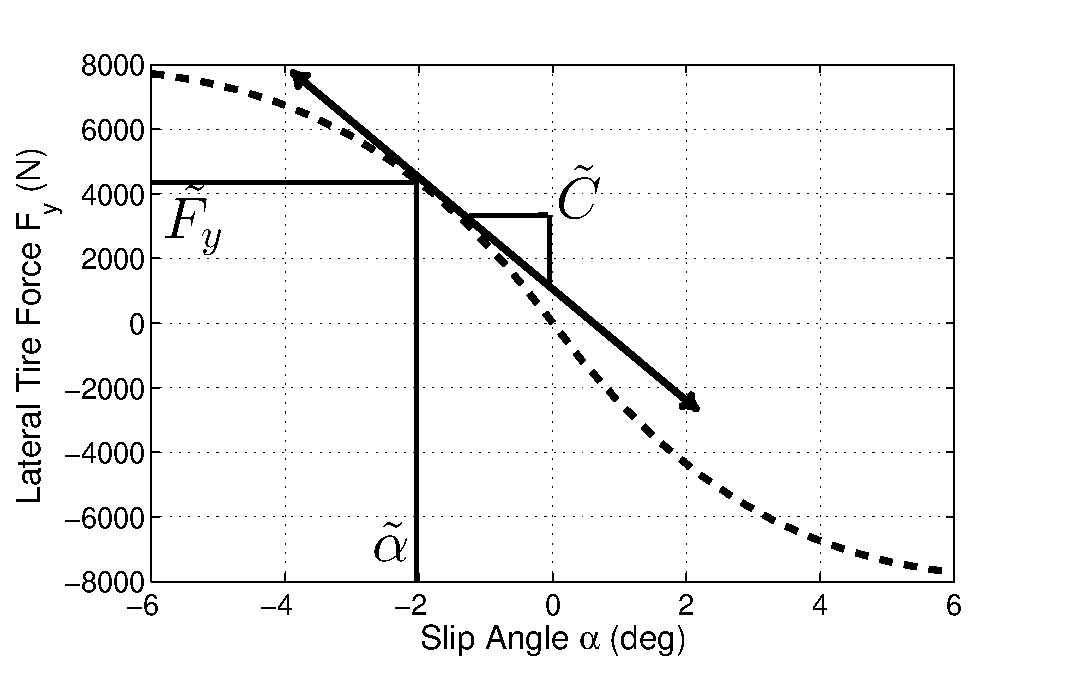
\includegraphics[width=.9\fullwidth]{fiala.eps}
\caption{Nonlinear tire force curve given by Fiala model, along with affine tire model linearized at $\alpha = \tilde{\alpha}$. }
\label{fig:fiala}
\end{figure}

The affine, continuous bicycle model with
steering input $\delta$ is then written in state-space form as:
\begin{subequations}
\label{eq:cts}
\begin{align}
	\dot{x}(t) &= A(t) x + B(t)\delta + d(t)\\
	 x &= [e \hspace{2mm} \Delta\Psi \hspace{2mm} r \hspace{2mm} \beta \hspace{2mm} \Psi]^T
\end{align}
\end{subequations}
where we have added a fifth state, vehicle heading angle $\Psi$, defined as the time integral of yaw rate $r$.
 This makes explicit computation of the minimum curvature path simpler. The state matrices $A(t)$, $B(t)$, and affine term $d(t)$ 
 are given by:
\begin{align}
A(t)  &= \left[\begin{matrix}
  0 & U_x(t) & 0 & U_x(t) & 0\\ 
  0 & 0 & 1 & 0 & 0 \\ 
  0 & 0  & \frac{-a^2\tilde{C}_\mathrm{f}(t)-b^2\tilde{C}_\mathrm{r}(t)}{U_x(t)I_\mathrm{z}} & \frac{b\tilde{C}_\mathrm{r}(t) - a\tilde{C}_\mathrm{f}(t)}{I_\mathrm{z}} & 0 \\
  0 & 0  & \frac{b\tilde{C}_\mathrm{r}(t)-a\tilde{C}_\mathrm{f}(t)}{mU_x^2(t)}-1 & \frac{-\tilde{C}_\mathrm{f}(t) - \tilde{C}_\mathrm{r}(t)}{mU_x(t)} & 0 \\
  0 & 0 & 1 & 0 & 0
 \end{matrix}\right] \\
B(t) &=[0 \hspace{2 mm} 0 \hspace{3 mm} \frac{a \tilde{C}_\mathrm{f}(t)}{I_\mathrm{z}} \hspace{3 mm}  \frac{\tilde{C}_\mathrm{f}(t)}{mU_x(t)} \hspace{3mm} 0]^T \\
d(t) &= \left[\begin{matrix} 0 \\
               -\kappa(t) U_x(t) \\ 
			    \frac{a\tilde{C}_\mathrm{f}(t)\tilde{\alpha}_\mathrm{f}(t) - b\tilde{C}_\mathrm{r}(t)\tilde{\alpha}_\mathrm{r}(t) + a\tilde{F}_\mathrm{yf}(t) - b\tilde{F}_\mathrm{yr}(t)}{I_z} \\
				\frac{\tilde{C}_\mathrm{f}(t)\tilde{\alpha}_\mathrm{f}(t) + \tilde{C}_\mathrm{r}(t)\tilde{\alpha}_\mathrm{r}(t) + \tilde{F}_\mathrm{yf}(t) + \tilde{F}_\mathrm{yr}(t)}{mU_x(t)}\\
				0
				\end{matrix}\right]
\end{align}

With the nonlinear model approximated as an affine, time-varying model, updating the path is accomplished by solving the following
 convex optimization problem:

\begin{subequations}
\label{eq:OPT}
\begin{alignat}{3}
\underset{\delta, \hspace{.5mm} x}{\text{minimize}} \quad & \sum_{k} \left(\frac{\Psi_k - \Psi_{k-1}}{s_k - s_{k-1}}\right)^2 + \lambda(\delta_k - \delta_{k-1})^2 & \quad  \label{eq:obj}\\
{\text{subject to}} \quad & \rlap{$ x_{k+1}= A_k x_k + B_k \delta_k + d_k$} \label{jenny}\\
& \rlap{$w^\mathrm{out}_k \leq e_k \leq w^\mathrm{in}_k $} \label{bobby}\\
& \rlap{$x_1 = x_T$\label{keylani}}
\end{alignat}
\end{subequations}
where $k = 1 \dots T$ is the discretized time index, and $A_k$, $B_k$, and $d_k$ are discretized versions of the continuous state-space
equations in (\ref{eq:cts}). The objective function (\ref{eq:obj}) minimizes the curvature norm of the path driven by the vehicle, as path curvature is
the derivative of the vehicle heading angle with respect to distance along the path $s$ (\ref{eq:balls}). To maintain convexity of the objective
function, the term ${s_k - s_{k-1}}$ is a constant rather than a variable, and is updated for the next iteration after the optimization has been completed (see \S \ref{sec:IMPLEMENT}).
Additionally, there is a regularization term with weight $\lambda$ added in the cost function to ensure a smooth steering profile for experimental 
implementation. 

\begin{figure}[h]
\centering
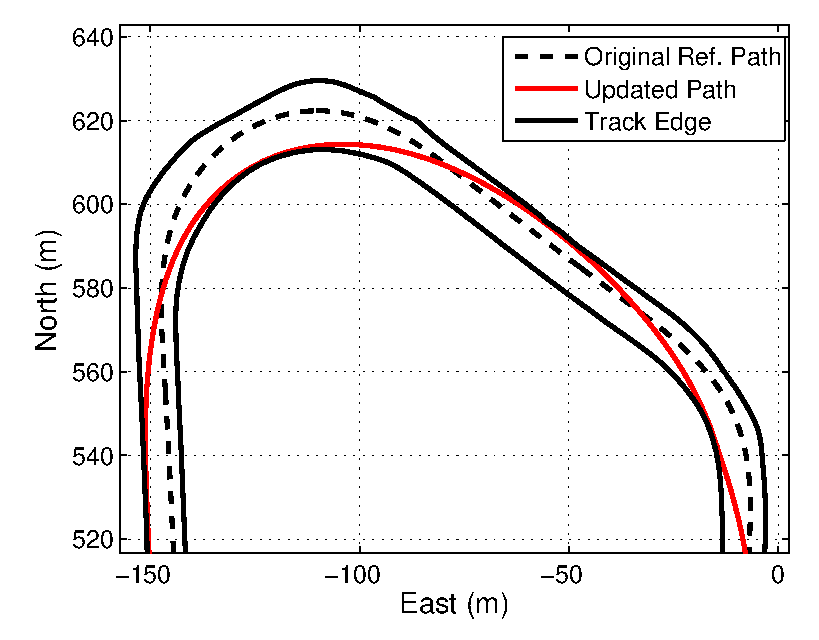
\includegraphics[width=.7\fullwidth]{updatedpath.eps}
\caption{Path update for an example turn.}
\label{fig:hairpin}
\end{figure}


The equality constraint (\ref{jenny}) ensures the vehicle follows the affine lateral dynamics. The inequality
 constraint (\ref{bobby}) allows the vehicle to deviate laterally from the reference path to find a new path with lower curvature, but
 only up to the road edges. Finally, the equality constraint (\ref{keylani}) is required for complete racing circuits to ensure the generated
 racing line is a continuous loop. The results of running the optimization 
 are shown for an example turn in Fig.~\ref{fig:hairpin}. The reference path starts out at the road centerline, and the optimization finds 
 a modified path that uses all the available width of the road to lower the path curvature. Note that the available road widths $w_\mathrm{in}$ and
 $w_\mathrm{out}$ have an offset built in to account for the width of the vehicle. 

 
\section{Algorithm Implementation and Simulated \newline Results}
\label{sec:IMPLEMENT}
\subsection{Algorithm Implementation}
The final algorithm for iteratively
generating a vehicle racing trajectory is described in Fig.~\ref{algorithmDesc}. 
The input to the algorithm is any initial path through the racing circuit, 
parameterized in terms of distance along the path $s$, path curvature $\kappa(s)$, and the lane edge distances $w_\mathrm{in}(s)$ and 
$w_\mathrm{out}(s)$ from Fig.~\ref{fig:worldInfo}.
 \begin{figure}
\begin{algorithmic}[1]
\Procedure{GenerateTrajectory}{$s^0, \kappa^0, w_\mathrm{in}^0, w_\mathrm{out}^0$}
\State $\mathrm{path}\gets (s^0, \kappa^0, w_\mathrm{in}^0, w_\mathrm{out}^0)$
\While{$\Delta t^\star > \epsilon$}
\State $U_x \gets \mathrm{calculateSpeedProfile(path)}$
\State $\mathrm{path} \gets \mathrm{minimizeCurvature}(U_x, \mathrm{path})$
\State $t^\star \gets \mathrm{calculateLapTime}(U_x,\mathrm{path})$
\EndWhile
\State \textbf{return} $\mathrm{path},U_x$
\EndProcedure
\end{algorithmic}
\caption[Iterative algorithm for fast generation of vehicle trajectories.]{Iterative algorithm for fast generation of vehicle trajectories. Each iteration consists of a sequential two-step approach where
the velocity profile is generated given a fixed path and then the path is updated based on the solution from a convex optimization problem.}\label{algorithmDesc}
\end{figure}

 Given the initial path, the minimum-time speed profile $U_x(s)$ is calculated using the
approach from \S \ref{sec:VP}. Next, the path is modified by solving the minimum curvature
 convex optimization problem (\ref{eq:OPT}). 
 

 
The optimization only solves explicitly for the steering input $\delta^\star$ and resulting vehicle lateral states $x^\star$ at every 
time step. Included within $x^\star$  is the optimal vehicle heading $\Psi^\star$ and lateral deviation $e^\star$ from the initial path. To obtain 
the new path in terms of $s$ and $\kappa$, the East-North coordinates ($E_k$, $N_k$) of the updated vehicle path are updated as follows:
	
\begin{subequations}
\begin{align}
	E_k &\gets E_k - e^\star_k\cos(\Psi_{\mathrm{r},k})\\
	N_k &\gets N_k - e^\star_k\sin(\Psi_{\mathrm{r},k})
\end{align}
\end{subequations}
where $\Psi_\mathrm{r}$ is the path heading angle of the original path. Next, the new path is given by the following numerical approximation:
 \begin{subequations}
 \label{eq:pupdate}
\begin{align}
	s_k &= s_{k-1} + \sqrt{(E_k - E_{k-1})^2 + (N_k - N_{k-1})^2}\\ 
	\kappa_k &= \frac{\Psi^\star_k - \Psi^\star_{k-1}}{s_k - s_{k-1}}
\end{align}
\end{subequations}
 Notice that (\ref{eq:pupdate}) accounts for the change in the total path length that occurs when the vehicle deviates from the original path.
 In addition to $s$ and $\kappa$, the lateral distances to the track edges $w_\mathrm{in}$ and $w_\mathrm{out}$ are different for the new path
 as well, and are recomputed using the Cartesian coordinates for
the inner and outer track edges and ($E_k$, $N_k$). The two-step procedure is iterated until the improvement in lap time $\Delta t^\star$ over the prior iteration is less than a small positive 
constant $\epsilon$.


\begin{table}
\label{tb:optprm}
\begin{center}
\small
\caption{Optimization Parameters}\label{tb:optprm}
\begin{tabular}{lccc}
Parameter & Symbol & Value & Units \\\hline
Regularization Parameter & $\lambda$ & 1 & $\mathrm{1/m}^2$\\
Stop Criterion           & $\epsilon $ & 0.1 & s \\
Vehicle mass & $m$ & 1500 & kg \\
Yaw Inertia & $I_z$ & 2250 & $\mathrm{kg \cdot m}^2$\\
Front axle to CG & $a$ & 1.04 & m\\
Rear axle to CG & $b$ & 1.42 & m\\
Front cornering stiffness & $\mathrm{C}_\mathrm{f}$ & 160 & $\mathrm{kN \cdot rad}^{-1}$ \\
Rear cornering stiffness & $\mathrm{C}_\mathrm{r}$ & 180 & $\mathrm{kN \cdot rad}^{-1}$ \\
Friction Coefficient     & $\mu $                  &  0.95 & $\mathrm{-} $ \\
Path Discretization      & $\Delta s$              & 2.75 & $m$\\
Optimization Time Steps  & $T       $              & 1843 & -  \\
Max Engine Force         & -                       & 3750 & N\\\hline
\end{tabular}
\end{center}
\end{table}

\subsection{Algorithm Validation}
The proposed algorithm is tested by analyzing the lap time performance on
 the same racing circuit and Audi TTS experimental test vehicle described in
Chapter 2. The vehicle parameters 
used for the lap time optimization are shown along with the optimization parameters in Table \ref{tb:optprm}.
 The initial path is obtained by collecting GPS data of the inner and outer track edges and estimating the ($s, \kappa, w_\mathrm{in}, w_\mathrm{out}$)
 parametrization of the track centerline via a separate curvature estimation subproblem similar to the one proposed in \cite{perantoni}.
 The algorithm is implemented in MATLAB, with the minimum curvature optimization problem (\ref{eq:OPT}) solved using the CVX software package \cite{boydcvx} and
 the speed profile generation problem solved using a library from Subosits and Gerdes \cite{subosits}.

 \begin{figure}
\centering
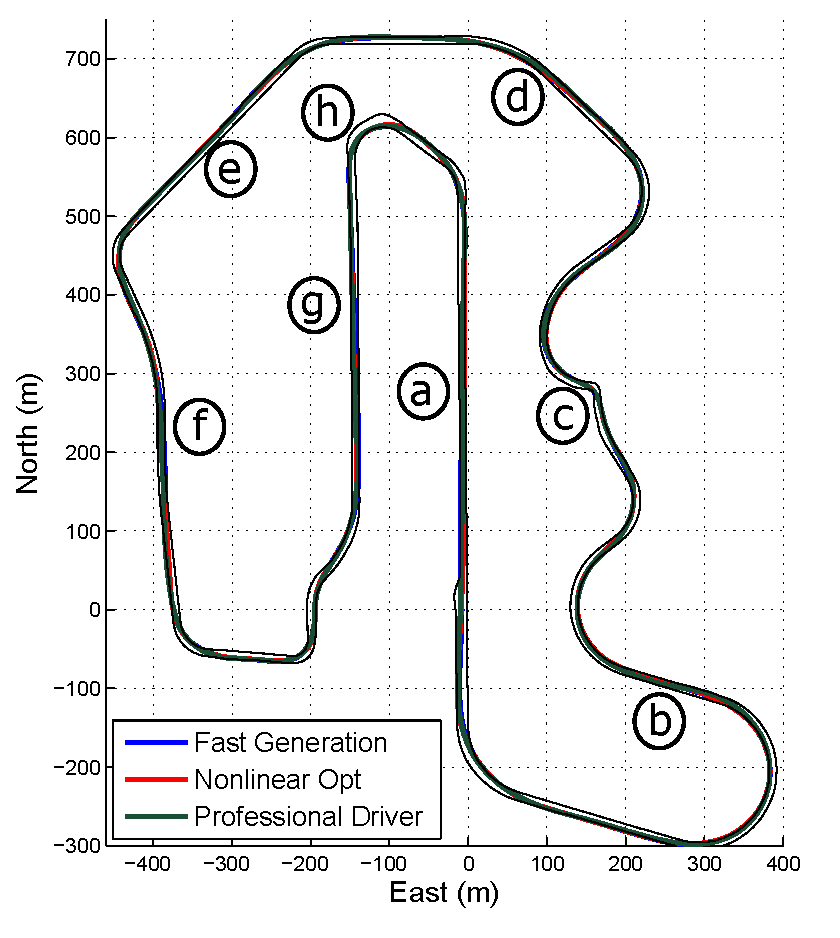
\includegraphics[width=\fullwidth]{racinglines.eps}
\caption[Overhead view of Thunderhill Raceway park along with generated path from algorithm.]{Overhead view of Thunderhill Raceway park along with generated path from algorithm. Car drives in alphabetical direction around the closed circuit. Labeled regions a-h are locations of discrepancies between the 
two-step algorithm solution and comparison solutions.}
\label{racingLines}
\end{figure}
\subsection{Comparison with Other Methods}
The generated racing path after five iterations is shown in
Fig.~\ref{racingLines}. To validate the proposed algorithm, the racing line is compared with results from a nonlinear gradient descent algorithm implemented by 
Theodosis and Gerdes \cite{theodosis} and an experimental trajectory recorded from a professional racecar driver in the experimental testbed vehicle.
 While time-intensive to compute, experimental lap times from the gradient descent trajectory are within one second of
lap times from professional racecar drivers. 

To better visualize the differences between all three racing lines, Fig.~\ref{fig:pathDeviation} shows the lateral deviation from the track centerline as a function of distance along the centerline 
for all three trajectories. The left and right track boundaries $w_\mathrm{in}$ and $w_\mathrm{out}$ are plotted as well. The two-step iterative algorithm provides a 
racing line that is qualitatively similar to the gradient descent and human driver racing lines. In particular, all three
solutions succeed at utilizing the available track width whenever possible, and strike similar apex points for each
of the circuit's 15 corners. 

\begin{figure}
\centering
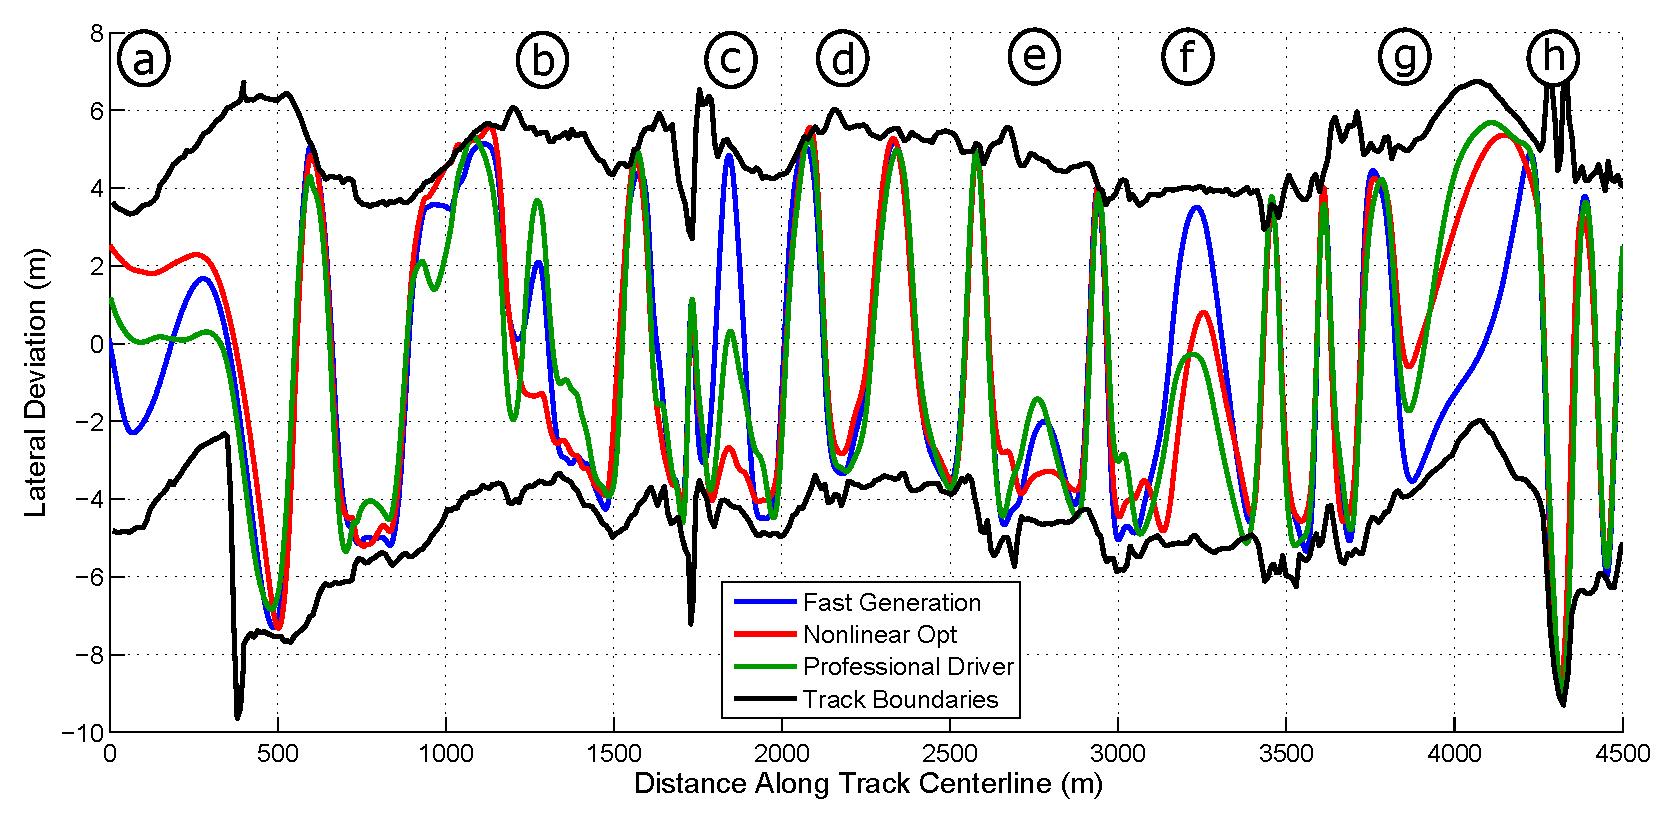
\includegraphics[width=\fullwidth]{deviationFromCenterline.eps}
\caption[Lateral path deviation of racing line from track centerline as a function of distance along the centerline.]{Lateral path deviation of racing line from track centerline as a function of distance along the centerline. Note that upper and lower bounds on $e$ are not always symmetric
due to the initial centerline being a smooth approximation. Results
are compared with racing line from a nonlinear gradient descent algorithm and experimental data recorded from a professional racecar driver.}
\label{fig:pathDeviation}
\end{figure}	

However, there are several locations on the track where there is a significant discrepancy (on the order of several meters) between the two-step algorithm's trajectory and the 
other comparison trajectories. These locations of interest are labeled \circled{a} through \circled{h} in Fig.~\ref{racingLines}.
Note that sections \circled{a}, \circled{e}, \circled{f}, and \circled{g} all occur on large, relatively straight portions of the racing circuit.
In these straight sections, the path curvature is relatively low and differences in lateral deviation from the track centerline have a relatively small
effect on the lap time performance.   

Of more significant interest are the sections labeled \circled{b}, \circled{c}, \circled{d}, and \circled{h}, which all occur at turning regions of the track.
These regions are plotted in Fig.~\ref{compositeFig1} and Fig.~\ref{compositeFig2} for zoomed-in portions of the race track. While it is difficult to analyze a single turn
of the track in isolation, discrepancies can arise between the two-step fast generation method and the gradient descent as the latter method trades off 
between minimizing curvature and distance traveled. As a result, the gradient descent method finds
 regions where it may be beneficial to use less of the available road width in order to reduce the total distance
traveled. In region \circled{b}, for example, the fast generation algorithm exits the turn and gradually approaches the left side in order to create space for the
upcoming right-handed corner. The nonlinear optimization, however, chooses a racing line that stays toward the right side of the track. 
In this case, the behavior of the human driver more closely matches that of the two-step fast generation algorithm.

 \begin{figure}[tb]
\centering
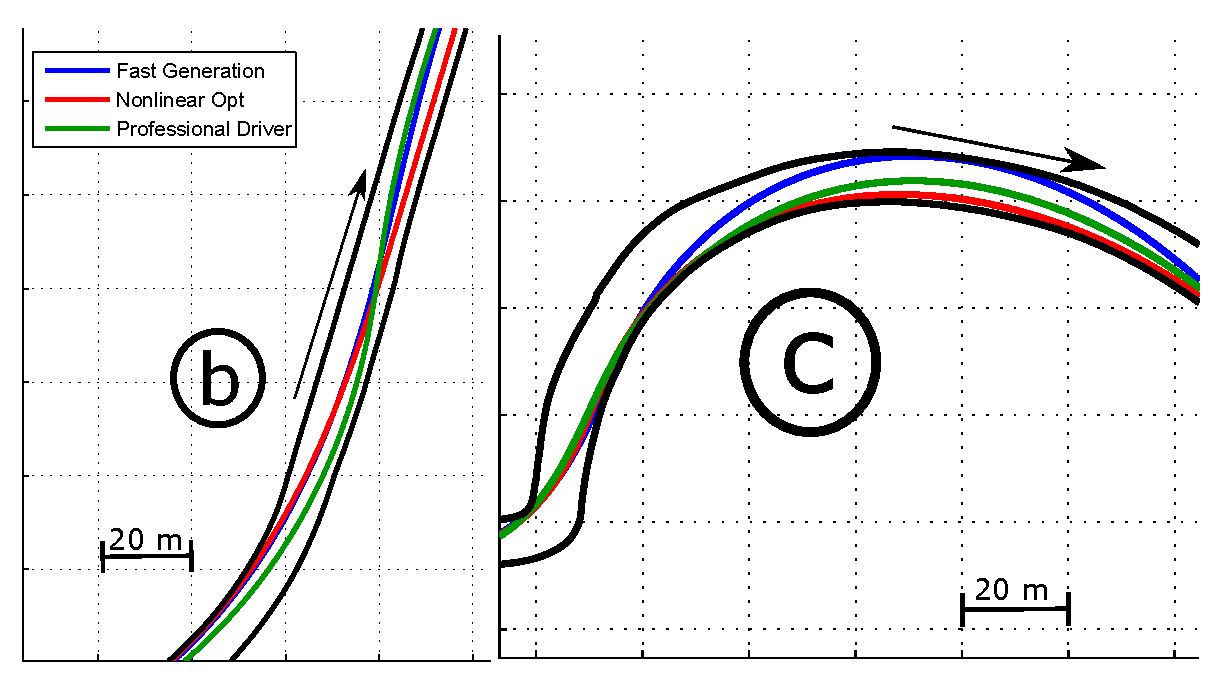
\includegraphics[width=\fullwidth]{composite1.eps}
\caption[Racing lines from the two-step fast generation approach, nonlinear gradient descent algorithm, and experimental data taken
from professional driver.]{Racing lines from the two-step fast generation approach, nonlinear gradient descent algorithm, and experimental data taken
from professional driver. Car drives in direction of labeled arrow.}
\label{compositeFig1}
\end{figure}

 \begin{figure}[tb]
\centering
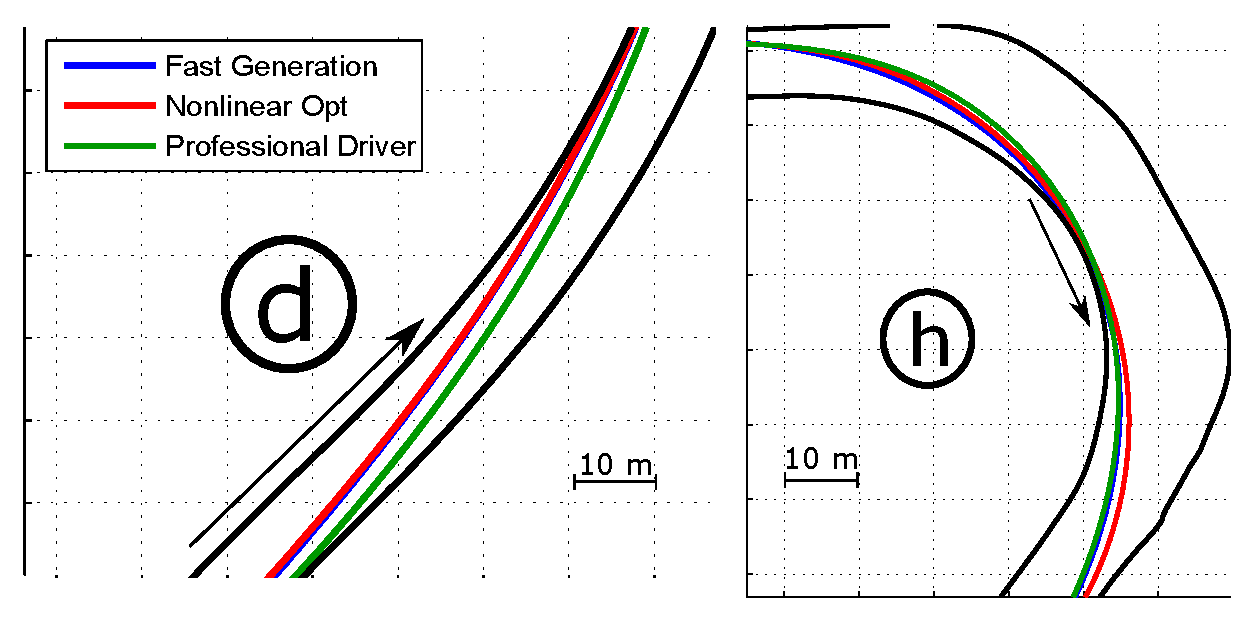
\includegraphics[width=\fullwidth]{composite2.eps}
\caption[Racing lines from the two-step fast generation approach, nonlinear gradient descent algorithm, and experimental data taken
from professional driver.]{Racing lines from the two-step fast generation approach, nonlinear gradient descent algorithm, and experimental data taken
from professional driver. Car drives in direction of labeled arrow.}
\label{compositeFig2}
\end{figure}	

 The human driver also drives closer to the 
fast generation solution in \circled{h}, while the gradient descent algorithm picks a path that exits the corner with a larger radius. In section \circled{c}, the gradient descent
algorithm again prefers a shorter racing line that remains close the the inside edge of the track, while the two-step algorithm drives all the way
to the outside edge while making the right-handed turn. Interestingly, the human driver stays closer to the middle of the road, but more closely
follows the behavior of the gradient descent algorithm. There are also regions of the track where the computational algorithms pick a similar path that 
differs from the human driver, such as region \circled{d}.
 
\subsection{Lap Time Convergence and Predicted Lap Time}
Fig.~\ref{lapTimes} shows the predicted lap time for each iteration of the fast generation algorithm, with step 0 corresponding
to the initial race track centerline. The lap time was estimated after each iteration by numerically simulating a vehicle 
 following the desired path and velocity profile using a closed-loop controller. The equations of motion for the simulation
were the nonlinear versions of (\ref{eq:bm}) with tire forces given by
the brush tire model in (\ref{eq:fiala}). 

\begin{figure}
\centering
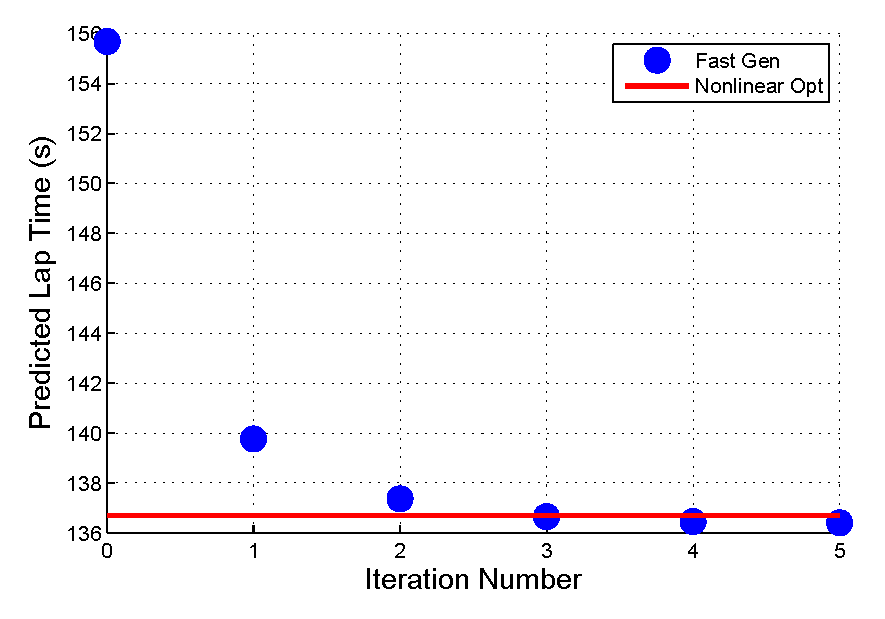
\includegraphics[width=.8\fullwidth]{laptimes.eps}
\caption[Lap time as a function of iteration for the two-step fast trajectory generation method.]{Lap time as a function of iteration number for the two-step fast trajectory generation method. Final lap time is comparable
to that achieved with the nonlinear gradient descent approach. Iteration zero corresponds to the lap time for driving the track centerline.}
\label{lapTimes}
\end{figure}

Fig.~\ref{lapTimes} shows that the predicted lap time converges monotonically over four or five iterations, with significant 
improvements over the centerline trajectory occuring over the first two iterations. The predicted minimum lap time of 136.4 seconds
is similar to the predicted lap time of 136.7 seconds from the nonlinear gradient descent, 
although in reality, the experimental lap time will depend significantly on unmodeled effects such 
as powertrain dynamics.  

The final curvature and velocity profile for the two-step  method is compared with the equivalent profiles for the gradient
descent algorithm in Fig.~\ref{fig:simData}. Notice that the piecewise linear $\kappa(s)$ for the gradient descent
 is due to the clothoid constraint imposed by \cite{theodosis} for ease of autonomous path following. 

 \begin{figure}[tb]
\centering
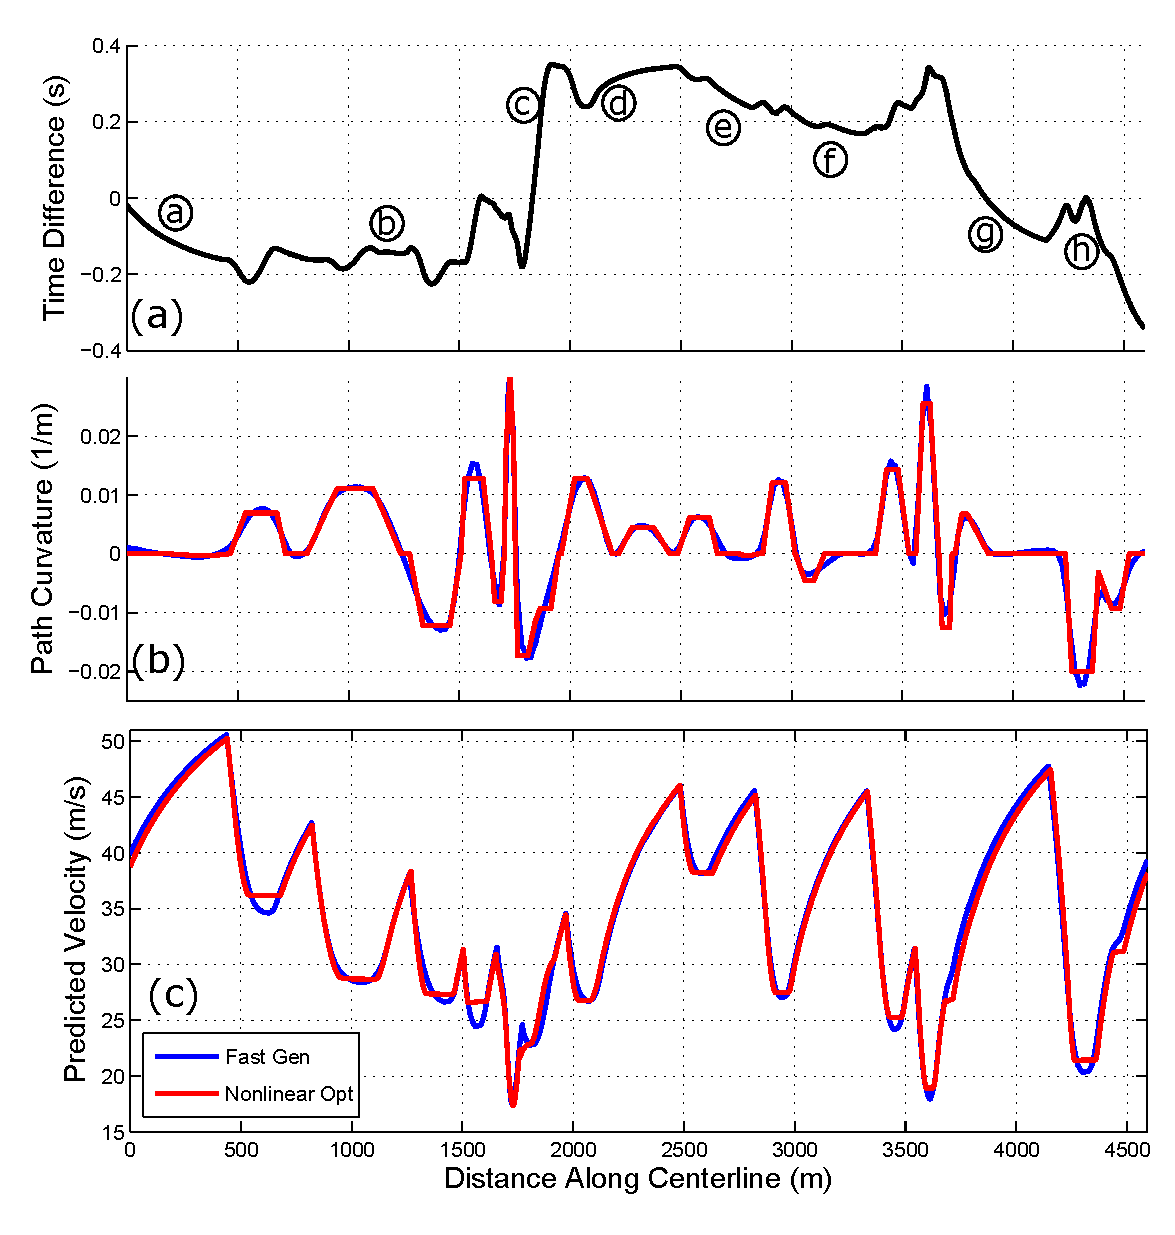
\includegraphics[width=\fullwidth]{simData.eps}
\caption[Simulation results of fast generation algorithm]{(a) Predicted time difference between a car driving both trajectories, with a negative
value corresponding the two-step algorithm being ahead. (b) Curvature profile $\kappa(s)$ plotted vs. distance along the path $s$.
 (c) Velocity profile $U_x(s)$ plotted 
vs. distance along the path $s$ for the two-step method and nonlinear gradient descent method.}
\label{fig:simData}
\end{figure} 
\newpage
In general, the curvature and velocity profiles are very similar, although the fast generation algorithm results in a velocity profile
with slightly lower cornering speeds but slightly higher top speeds.
The predicted time difference between a car driving both trajectories 
is shown in Fig.~\ref{fig:simData}(a), with a negative
value corresponding the two-step algorithm being ahead. 

Notice that in region \circled{c}, the trajectory from the two-step algorithm performs
poorly, losing almost a half second of time to the nonlinear optimization over just 150 meters. Referring back to Fig.~\ref{compositeFig1}, 
region \circled{c} is a sweeping right-hand turn that comes after a very tight left-hand turn on the track, and both the human driver
and nonlinear optimization prefer to take a shorter path and stay closer to the inside edge of the track. While this results in a higher
curvature for the first turn, the shorter path on the second turn creates a net time advantage. As a result, the gradient descent optimization from Theodosis
and Gerdes \cite{theodosis} retains an overall time advantage from this turn
on until losing ground in section \circled{g}, where the two-step method catches up and ultimately completes the lap with a 0.3 second time advantage. 
The difference between the two techniques suggests that neither is a globally optimal solution, since the minimum curvature heuristic proposed here and the restriction
to clothoid segments in \cite{theodosis} are not mutually exclusive and benefits of both could be combined to further improve the lap time. 

\section{Experimental Setup} 
\label{sec:EXP}
While the two-step algorithm works well in simulation, the most critical validation step is to have an
autonomous race car drive the generated trajectory. This was accomplished by 
collecting experimental data on the Audi TTS.  

The experimental controller setup is shown in Fig.~\ref{fig:expSetupC3} 
and is very similar to that presented in Chapter 2. The main two differences in the controller are highlighted
in red. Instead of using the piecewise linear clothoid  curvature profile from Theodosis and Gerdes \cite{theodosis}, the trajectory
from the presented algorithm is applied. This trajectory is 
represented mathematically as an array of discrete points. This point cloud is relatively
dense, with each point spaced about 25 cm apart over the entire path.

Since the trajectory is now a set of discrete points rather than a piecewise linear $\kappa(s)$ function, the localization algorithm cannot rely on Newton-Raphson gradient descent. Instead, a
simple search algorithm iterates through the point cloud and finds the closest two points to the vehicle's center of
gravity. Bisection is applied to the find the closest distance between the vehicle and the line connecting these
two points on the point cloud. To save the expense of searching the entire point cloud on every iteration, 
the localization starts the search algorithm where the last iteration terminated and searches only a small region
of the entire map. 

\begin{figure}[tb]
\centering
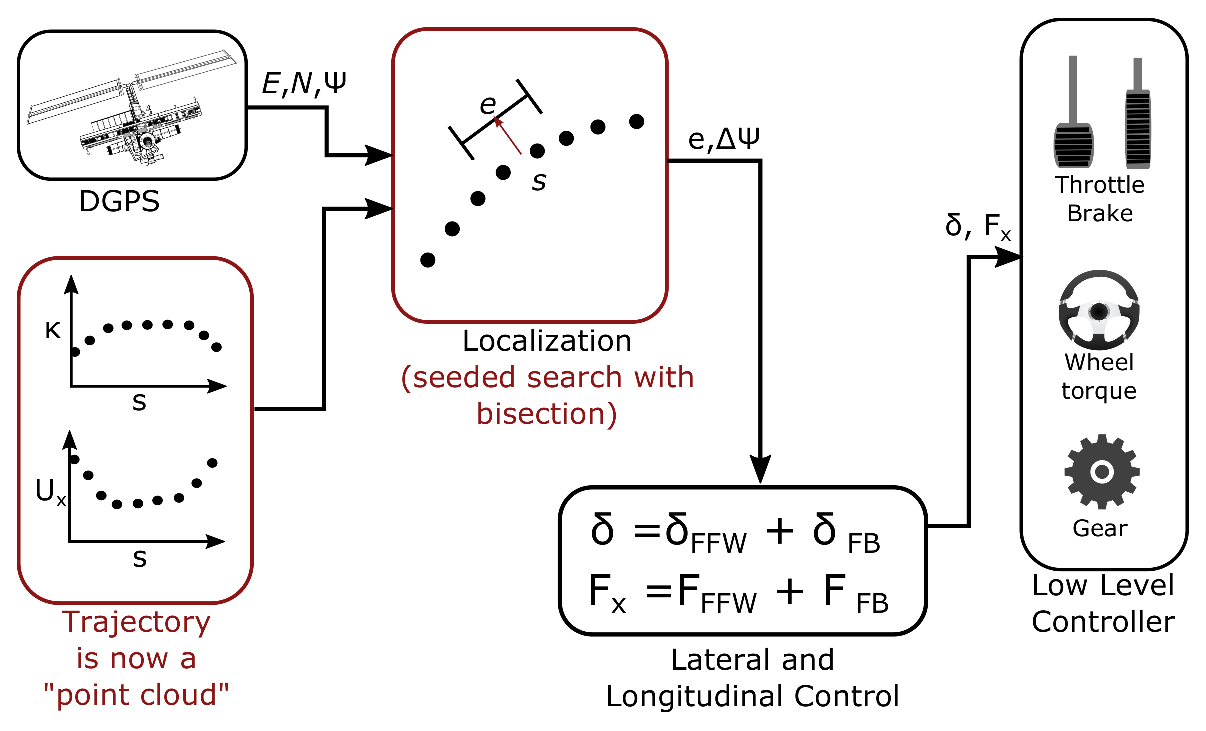
\includegraphics[width=\fullwidth]{expSetupC3.eps}
\caption{Diagram of controller setup.}
\label{fig:expSetupC3}
\end{figure}

\section{Experimental Results}
\label{sec:ch3ExpRes}

The resulting experimental lap time for the iterative two-step algorithm was 138.6 seconds, about 0.6 seconds faster
than the experimental lap time for the gradient descent algorithm (139.2 seconds). For safety reasons, the trajectories were generated using a conservative peak road friction value of $\mu = 0.90$,
 resulting in peak lateral and longitudinal accelerations of 0.9$g$. In reality, the true friction value of the road varies slightly, but is closer to $\mu = 0.95$ on average. As a
result, both of these lap times are slightly slower than the fastest lap time recorded by a professional race car driver (137.7 seconds) and
 the predicted lap times from Section \ref{sec:IMPLEMENT}. A summary of all lap times is provided in Table \ref{tb:laptimes}.

\begin{table}[tb]
\begin{center}
\begin{tabular}{c|cc}
    & Simulation & Experiment \\\hline
Fast Generation& 136.4 & 138.6 \\
Gradient Descent&  136.7 & 139.2 \\
Human Driver& N/A & 137.7 \\\hline
\end{tabular}
\caption{Lap Times in Seconds}\label{tb:laptimes}
\end{center}
\end{table}
   
Plots of the experimental data are shown in Fig.~\ref{fig:expdata}, with a negative time difference again corresponding to the two-step algorithm being ahead.
The experimental data generally matches the simulated results in Fig.~\ref{fig:simData}. The simulation predicted the trajectory from the iterative two-step algorithm would be 0.3 seconds
 shorter than that of the nonlinear algorithm, compared to the 0.6 second speed advantage observed experimentally. 
 The simulation also predicted a relative time advantage for the two-step algorithm from sections \circled{a} to \circled{c}
 and from \circled{e} to \circled{h}, a trend seen in the experimental data as well. Additionally, the
 two-step algorithm has relatively poor performance
 from sections \circled{c} to \circled{d} when compared to the nonlinear algorithm.  This experimental result
 confirms that the minimum curvature heuristic works well for the majority of the track, but relatively poorly on particular ``irregular" 
 sequences of turns such as region \circled{c}. Section \ref{sec:ADDMINDIST} will show the benefit of adding a term in the convex optimization
 cost function to consider distance traveled in addition to path curvature.
 
 One reason for minor variations between the simulated and experimental time difference plots is variation in speed tracking. 
 The speed tracking error for both racing lines is shown in Fig.~\ref{fig:expdata}(c). Interestingly, while the same speed tracking controller was used to test both racing lines, 
 the controller has slightly better speed tracking performance when running the trajectory from the nonlinear optimization. This is possibly due to the
 longitudinal controller gains being originally tuned on a clothoid trajectory. 

 \begin{figure}[tb]
\centering
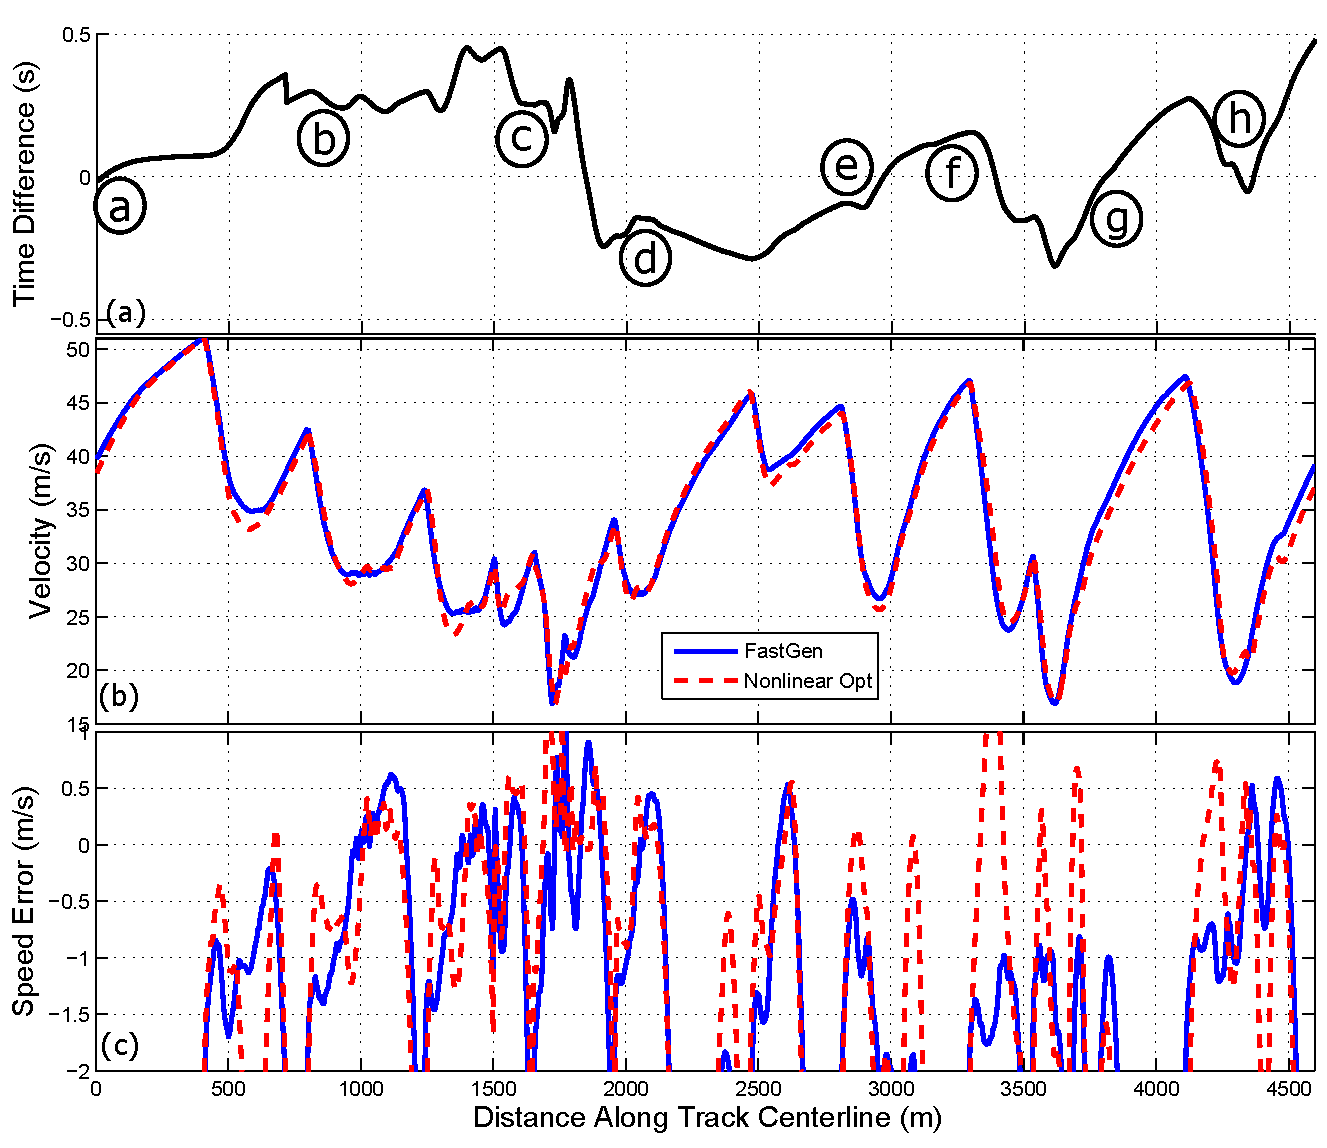
\includegraphics[width=\fullwidth]{expdata.eps}
\caption[Experimental data for an autonomous vehicle driving the trajectories provided by the two-step fast generation and gradient descent algorithms.]{Experimental data for an autonomous vehicle driving the trajectories provided by the two-step fast generation and gradient descent algorithms.(a) Relative time difference
between vehicle driving both trajectories, with a negative time difference corresponding to the two-step algorithm being ahead. (b) Actual
recorded velocity of vehicle. (c) Difference between actual and desired speed. Large negative values outside plotting range occur 
 on straight sections of the track where the vehicle is limited by engine power and speed tracking error is poorly defined. (d) Throttle percentage and brake pressure, with brake pressures shown as negative.  }
\label{fig:expdata}
\end{figure}

\section{Incorporating the Effect of Distance Traveled}
\label{sec:ADDMINDIST}
The performance of the presented trajectory generation approach can be further improved by modifying the cost function (\ref{eq:OPT})
of the path update step. Instead of only minimizing curvature, a new convex cost function is proposed\footnote{Special thanks to John K. Subosits for help deriving this modified cost function.} that minimizes a weighted
sum of the distance traveled and the path curvature. While this also does not directly minimize lap time, it does account for the incremental benefit provided by a shorter
path, which may be helpful in improving the performance of the algorithm on particular turns such as region \circled{c}.

A convex term for the total distance traveled by the race vehicle is derived as follows. The instantaneous rate of
 progress of the vehicle along a fixed path is given by:
\begin{equation}
	\dot{s} = \frac{U_x}{1-ke}\cos(\Delta\Psi + \beta)
\end{equation}
and the time to travel between two fixed points on the nominal path is given by:

\begin{equation}
t_k = \frac{s_k - s_{k-1}}{\dot{s}_k}
\end{equation}
Since the  path discretization $s_k - s_{k-1}$ and speed profile $U_x$ are fixed during the path update step , minimizing path length is equivalent to
minimizing the sum over all $t_k$:
\begin{equation}
	\sum_k \frac{s_k-s_{k-1}}{U_{xk}} \left(\frac{1-\kappa_ke_k}{\cos(\Delta \Psi_k + \beta_k)}\right)
\end{equation}
Taking the Taylor series expansion in the optimization variables ($e, \Delta\Psi, \beta$) for the path update step yields a convex approximation
 for minimizing the distance
traveled by the vehicle:
\begin{equation}
	\label{eq:minDist}
	\sum_k \frac{\Delta s_k}{U_{xk}} \left(-\kappa_ke_k + (\Delta\Psi_k + \beta_k)^2\right)
\end{equation}
The first term $-\kappa_ke_k$ in (\ref{eq:minDist}) rewards moving to the inside of curved sections, and the
second term $(\Delta\Psi_k + \beta_k)^2$ represents the additional distance traveled when driving at an angle to the original path.  

\subsection{Balancing Minimum Distance and Curvature}
\label{sec:ch3balance}

Minimizing (\ref{eq:minDist}) subject to the vehicle dynamics and road boundary constraints from (\ref{eq:OPT}) results in the path shown in Fig.~\ref{fig:minDist}.
As expected, the resulting path simply clings to the inner edge of the track wherever possible. A simple glance shows that entirely minimizing
distance traveled generates an extremely poor racing line. In fact, the resulting simulated lap times are over ten seconds slower than the minimum distance
solution! 

 \begin{figure}
\centering
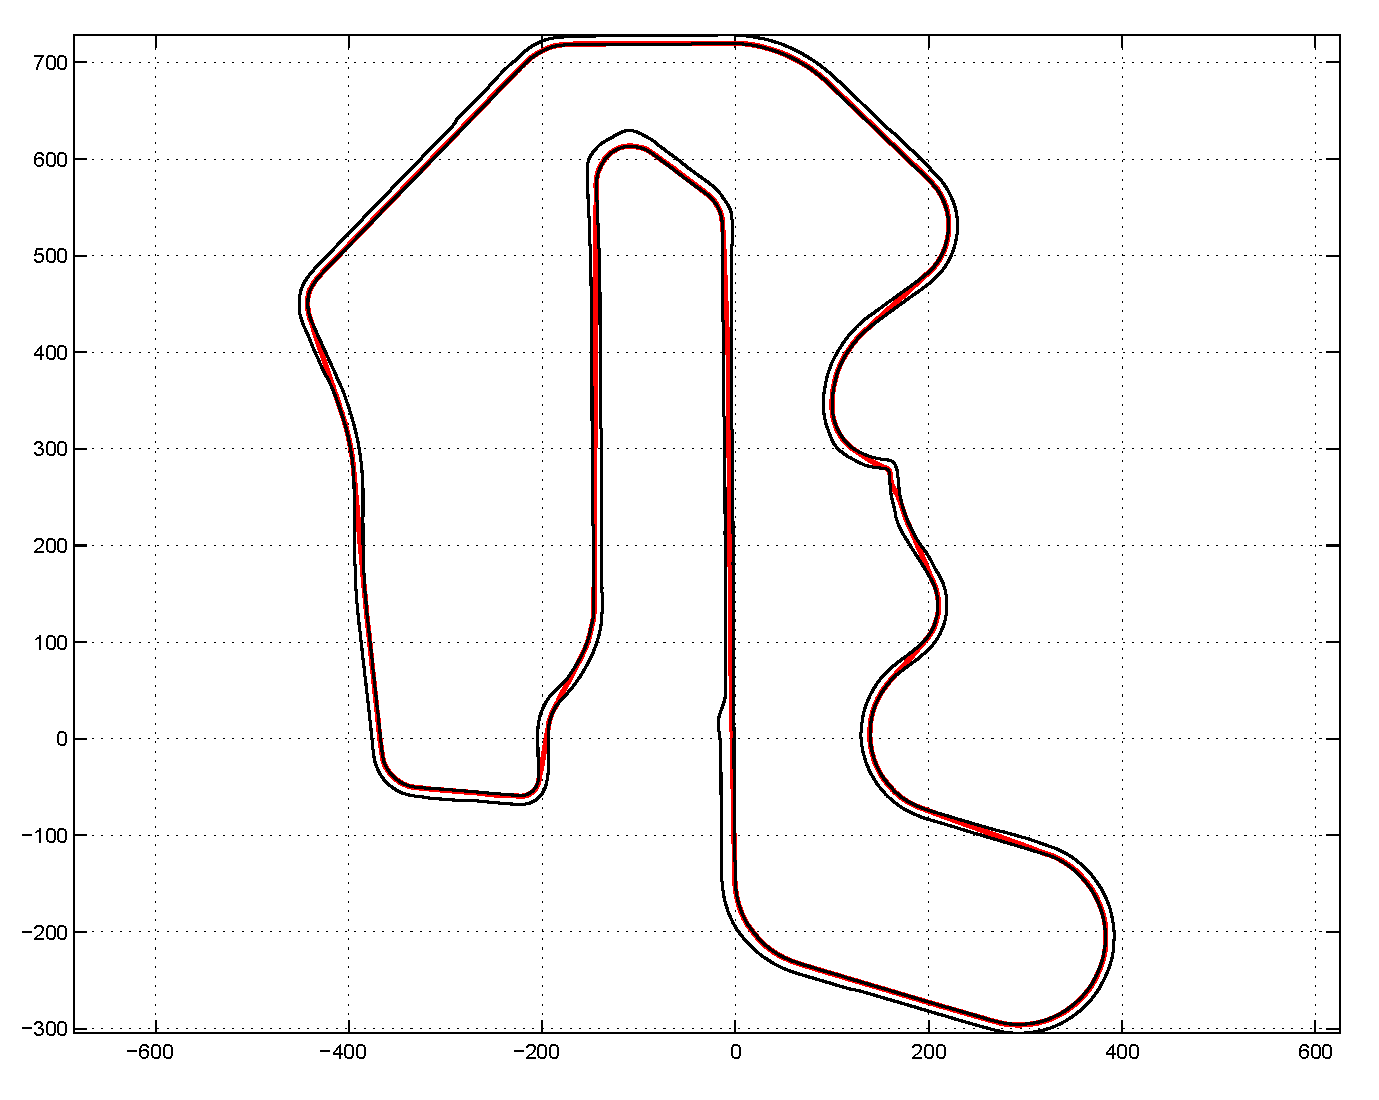
\includegraphics[width=\fullwidth]{shortestpath.eps}
\caption{Minimum distance path around Thunder Hill}
\label{fig:minDist}
\end{figure}

There is clearly a need for a balance between minimizing distance and minimizing curvature, weighted more significantly towards the latter. There have been
several prior attempts in the literature to perform this balance. Braghin \cite{braghin} proposed finding the minimum distance and minimum curvature paths through 
a purely geometric optimization, with no vehicle dynamics considered. Weighted combinations of these
basis paths were then generated and tested using a simple point mass model. For example, let $e_D(s)$ denote the lateral offsets from the track centerline corresponding to the minimum
distance path. Then let $e_\kappa(s)$ be the corresponding offsets for the minimum curvature path. A proposed racing line is then defined by:

\begin{equation}
e = (1-\eta)e_\kappa + \eta e_D
\end{equation}

Where $0 \leq \eta \leq 1$ is the weighting parameter. Figure~\ref{fig:linearCombos} demonstrates this concept for the Thunderhill Racing Circuit. Racing lines generated
with $\eta$ close to 0 are very similar to the minimum curvature path, while candidate solutions with $\eta$ close to 1 approximate the minimum distance path. 

 \begin{figure}
\centering
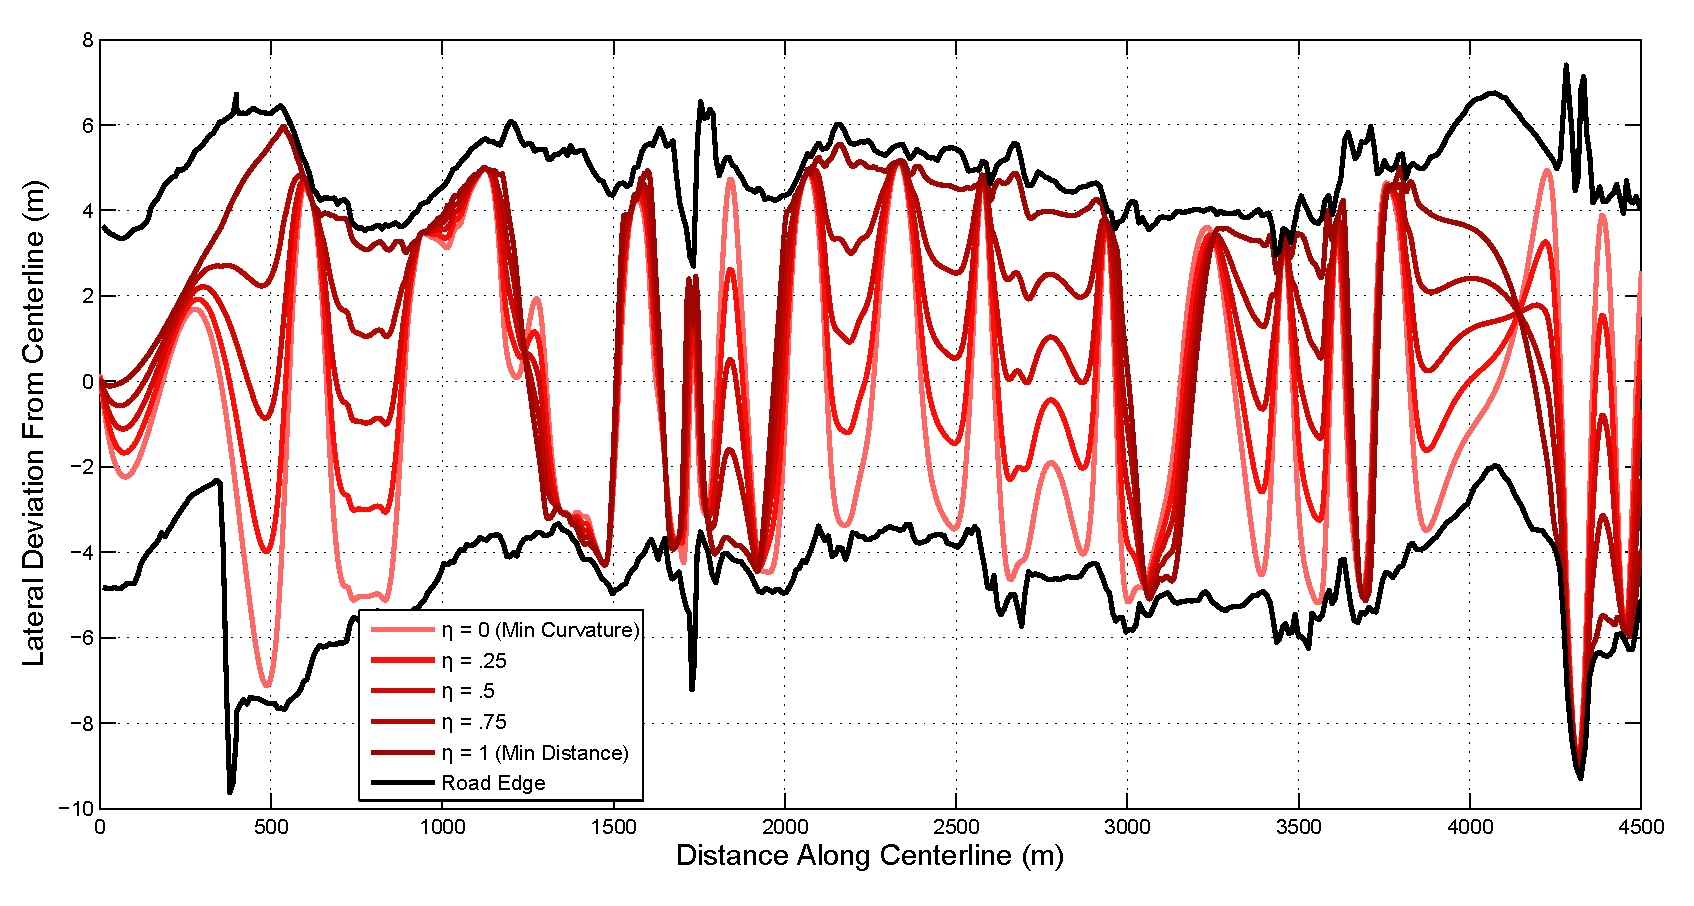
\includegraphics[width=\fullwidth]{linearCombinations.eps}
\caption{A family of racing lines generated from linear combinations of minimum distance and minimum curvature racing lines, with weighting parameter $\eta$.}
\label{fig:linearCombos}
\end{figure}

The issue with this approach is that a single weighting parameter $\eta$ does not adequately balance the tradeoff between minimizing distance and minimizing curvature.
On most sections of a given track, the primary objective is simply to minimize curvature. However, there are typically a small minority of turns (for example, region \circled{c} in our 
case) where minimizing distance traveled is relatively important. A better method is therefore to have the weighting parameter $\eta$ be a function $\eta(s)$ that varies
along the track. This is exactly the approach suggested by Cardamone et al. \cite{cardamone}, who analyzed Braghin's approach over a number of tracks and found that
if only a single weighting factor was chosen, the optimal solution was frequently just $\eta = 0$ (i.e. the minimum curvature path).  

Cardamone et al. suggested determining $\eta(s)$ by applying a genetic algorithm to choose a different weighting parameter between every intersection of the minimum curvature
and minimum distance paths. Similar approaches were also presented by Gadola et al. \cite{gadola} and M{\"u}hlmeier and M{\"u}ller \cite{mully}.
While this provided improved lap times over the minimum curvature solution, genetic algorithms are typically slow computationally, as every candidate solution $\eta(s)$ must be
 simulated. The computational benefit over nonlinear programming that directly minimizes lap time is therefore debatable. 
 
\subsection{Using Human Driver Data to Obtain Optimization \newline Weights}
Using professional driver data as a baseline offers a simpler method to determine parts of the track where minimizing distance is important. Fig.~\ref{fig:DKtrade}(a) shows ten
laps of human driver data on the Thunderhill racetrack overlaid onto Figure~\ref{fig:linearCombos}. Fig.~\ref{fig:DKtrade}(b) shows the resulting weighting
function $\eta(s)$ obtained by averaging the human data and finding the relative distance from the human centerline deviation $e_H(s)$ to the minimum curvature and
minimum distance solutions:

\begin{equation}
\eta(s) = \frac{|e_H(s) - e_\kappa(s)|}{|e_H(s) - e_D(s)|}
\end{equation} 

 \begin{figure}[h!]
\centering
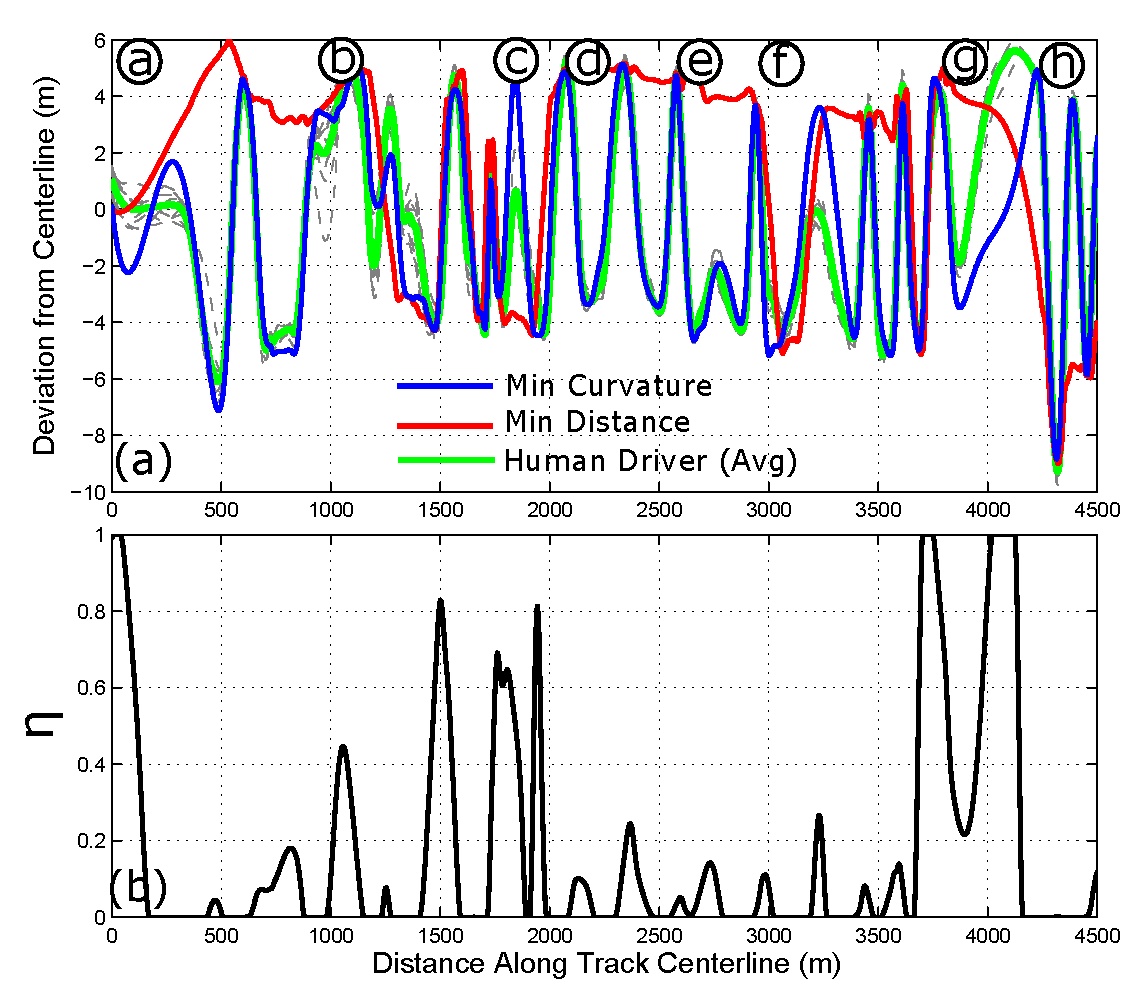
\includegraphics[width=\fullwidth]{distCurvatureTradeoff.eps}
\caption[Ten laps of professional human driver data overlaid over the minimum distance and minimum curvature solutions]{(a) Ten laps of professional human driver data overlaid over the minimum distance and minimum curvature solutions $e_D(s)$ and $e_\kappa(s)$. The average of the human driver
data is shown in green, and the individual datasets are shown in light grey. (b) Values of $\eta(s)$ from human data, with low pass filter applied to eliminate rapid changes. Values are also limited to range from 0 to 1.}
\label{fig:DKtrade}
\end{figure}

\newpage
This definition is only relevant if the human racing line is bounded by the minimum distance and minimum curvature racing lines. Since this is frequently not
the case in Fig.~\ref{fig:DKtrade}(a), $\eta(s)$ is set to 1 if $e_H(s) < e_D(s) < e_\kappa(s)$ or 0 if $e_H(s) < e_\kappa(s) < e_D(s)$. Furthermore, a low-pass filter is also applied to Fig.~\ref{fig:DKtrade}(a) to eliminate rapid changes in $\eta(s)$.

Fig.~\ref{fig:DKtrade} shows that there are several regions of the track where the human drives closer to to the minimum distance racing line (i.e. locations where
$\eta$ is significantly greater than 0). Most of these are trivial, occurring in locations where the minimum distance and minimum curvature racing lines are
relatively close. However, in region \circled{c}, the professional human driver is on average about halfway between the minimum distance and minimum curvature solutions,
an interesting result. Furthermore, on straight sections of the track such as \circled{a} and \circled{g}, the human driver appears to be seeking a minimum distance path as well. 

\subsection{Combined Cost Function and Simulated Results}

Using the information from Fig.~\ref{fig:DKtrade}, the combined cost function for the path update step in (\ref{eq:OPT}) is given by:

\begin{equation}
\label{eq:OPT2}
\underset{\delta, \hspace{.5mm} e, \hspace{.5mm} \Psi, \hspace{.5mm} \Delta\Psi, \hspace{.5mm} \beta}{\text{minimize}} \quad \sum_{k} \left(\frac{\Psi_k - \Psi_{k-1}}{s_k - s_{k-1}}\right)^2 + \lambda\sum_k \frac{\eta_k \Delta s_k}{U_{xk}} \left(-\kappa_ke_k + (\Delta\Psi_k + \beta_k)^2\right)
\end{equation}

The first summation in (\ref{eq:OPT2}) is the same curvature minimization term, while the second summation represents the distance minimization term. The weights
$\eta_k$ from Fig.~\ref{fig:DKtrade}(a) are used to determine how much of the minimum distance term to use at each point along the track. This approach is fundamentally
different from the methods in \cite{braghin} and \cite{cardamone}. The prior approaches search a space of solutions to find the best linear combination of the \textit{pre-calculated} minimum distance and minimum curvature racing
lines, with weights given by a constant $\eta$ or function $\eta(s)$. The presented approach performs a single optimization for each path update step, with the \textit{optimization weights} given by $\eta_k$. As a result, there is 
an additional tunable parameter $\lambda$ in (\ref{eq:OPT2}) with units of seconds, that ensures units of both summation terms are the same.

There are several benefits of the proposed approach. First, since we obtained $\eta(s)$ from human driver data, simply applying a linear combination with weights $\eta(s)$ would
trivially give back the averaged professional driver's racing line. More importantly, however, using pure linear combinations of two precomputed solutions provides excessive restrictions on the resulting racing lines. 
This is because the resulting solutions can never explore regions that are not contained within the minimum curvature and minimum distance solutions. Furthermore, there is no guarantee the resulting path will be experimentally drivable. 
Even if the minimum curvature and distance paths come from an optimization with vehicle dynamics constraints, if the weighting function $\eta(s)$ is not sufficiently smooth, there will be discontinuities in
the resulting curvature profile. By using $\eta(s)$ to instead guide the optimization, the resulting curvature profile will always be smooth. 


 \begin{figure}
\centering
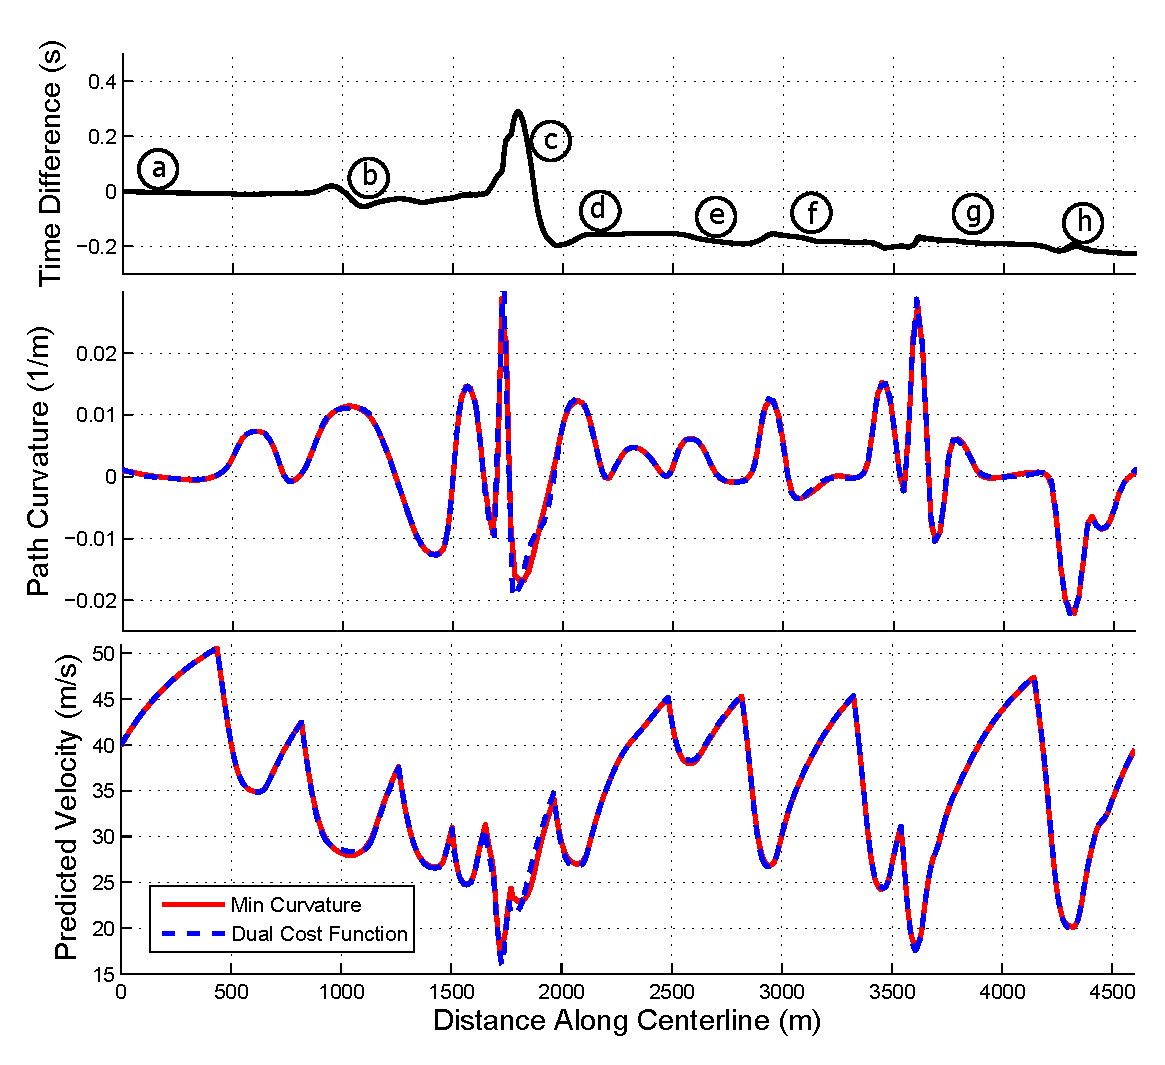
\includegraphics[width=\fullwidth]{simWithMinDist.eps}
\caption[Simulation results comparing minimum curvature cost function with weighted cost function]{Simulation results comparing minimum curvature cost function with weighted distance/curvature cost function ($\lambda = 0.05$ sec). (a) Time difference between two solutions as a function
of distance along centerline, with a negative time
difference corresponding to the weighted optimization being ahead. (b) Path curvature. (c) Simulated velocities.}
\label{fig:SD2}
\end{figure}

Fig.~\ref{fig:SD2} shows simulation results when the fast generation method is run for five iterations. The simulation compares the racing lines
 generated by the curvature minimization cost function and the combined curvature-distance cost functions. 
Unsurprisingly, the primary difference occurs at region \circled{c}. With the combined cost function, the resulting racing line takes a slightly higher curvature turn on the initial left turn. While this
initially loses time, the resulting solution can minimize distance traveled on the next turn, resulting in an overall time advantage of 0.2 seconds. 

 \begin{figure}
\centering
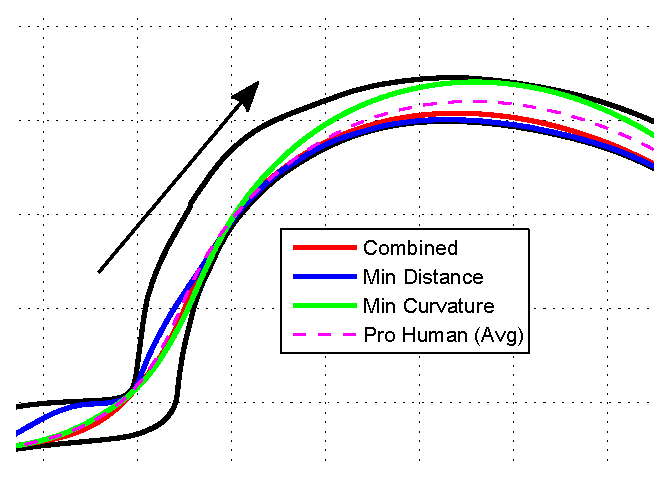
\includegraphics[width=.7\fullwidth]{regC.eps}
\caption[Racing lines for minimum curvature, minimum distance, and combined cost functions around region c.]{Racing lines for minimum curvature, minimum distance, and combined cost functions around region c. Notice that with the combined cost function,
the resulting racing line is not bounded by the minimum curvature and minimum distance solutions. Averaged pro human racing line is shown as well.}
\label{fig:regC}
\end{figure}

The minimum distance,
minimum curvature, and combined racing lines at region \circled{c} are shown in Fig.~\ref{fig:regC}. The combined solution follows the minimum curvature solution more
closely for the initial left-hand turn, but the minimum distance solution more closely for the second right-hand turn. Additionally, the racing line
from the dual cost function is not always inside the minimum distance and minimum curvature racing lines. This demonstrates the advantage of a weighted cost function
as opposed to a linear combination of pre-calculated solutions.  

\section{Discussion and Future Work}
\label{sec:DISCUSSION}

The primary benefit of the proposed algorithm is not improved lap time performance
over the nonlinear algorithm but rather a radical improvement in computational simplicity and speed. Each two-step iteration of the full
course takes only 26 seconds on an Intel i7 processor, whereas the nonlinear algorithm from \cite{theodosis} typically runs over the course of several hours on the same
machine. The most significant computational expense for the proposed algorithm is solving the convex curvature minimization problem for
all 1843 discrete time steps $T$ over the 4.5 km racing circuit.

\begin{table}[h]
\begin{center}
\caption{Iteration Computation Time}\label{tb:solvetime}
\begin{tabular}{ccc}
Lookahead (m) & $T$ & Solve Time (s) \\\hline
450& 184 &5 \\
900&  369 & 6 \\
1800& 737 & 12 \\
4500& 1843& 26 \\\hline
\end{tabular}
\end{center}
\end{table}

This computational efficiency will enable future work to incorporate the trajectory modification algorithm as an online
 ``preview" path planner, which would provide the desired vehicle trajectory for an upcoming portion of the race track. 
 Since the computation time of the algorithm is dependent on the preview distance, 
 the high-level planner would not need to run at the same sample time as the vehicle controller. Instead, the planner would operate on a separate CPU and provide a velocity profile and racing line for only
 the next 1-2 kilometers of the race track every few seconds, or plan a path for the next several hundred meters within a second.
 
 Table \ref{tb:solvetime} shows problem solve times for a varying range of lookahead lengths with the same discretization $\Delta s$,
 and shows that the runtime scales roughly linearly with the lookahead distance. The above solve times are listed using the CVX convex optimization solver, which 
 is designed for ease of use and is not optimized for embedded computing. Preliminary work has been successful
 in implementing the iterative two-step algorithm into C code using the CVXGEN software tool \cite{boydcvxgen}. When written
 in optimized C code, the algorithm can solve the curvature minimization problem (\ref{eq:OPT}) in less than 0.005 seconds for a lookahead distance of 650 meters.
 
 The possibility of real-time trajectory planning for race vehicles creates several fascinating areas of future research. An automobile's surroundings are subject to both rapid and
 gradual changes over time, and adapting to unpredictable events requires an approximate real-time trajectory planning algorithm.
 On a short time scale, the real-time trajectory planner could find a fast but stable recovery trajectory in the event of the race vehicle entering an understeer or oversteer 
 situation. On an intermediate time scale, the fast executing two-step algorithm could continuously plan a racing line in the presence of other moving race vehicles by constraining the
 permissible driving areas to be collision-free convex ``tubes" \cite{erlien}.  Finally, the algorithm could update the trajectory given estimates of the friction coefficient and other vehicle parameters learned gradually over
 time.
 
\section{Conclusion}
This chapter demonstrates an iterative algorithm for quickly generating vehicle racing trajectories, where each iteration is comprised of
 a sequential velocity update and path update step. Given an initial path through the race track, the 
 velocity update step performs forward-backward integration to determine the minimum-time speed inputs. Holding this speed 
 profile constant, the path geometry is updated by solving a convex optimization problem to minimize path curvature.

 The primary benefit of the presented trajectory planner is computational speed. Experimental data on an autonomous race vehicle over a
 three mile race course confirms that the trajectory generated by the algorithm provide comparable lap times to that from a nonlinear gradient descent algorithm. However, the
 required computation time is at least two orders of magnitude faster. One drawback of the presented approach is that lap time is not explicitly minimized, resulting
 in sub-optimal performance on complex sequences of turns. A second analysis was therefore conducted in simulation to show the
 benefit of adding a distance minimizing term to the convex path update step. An exciting opportunity for future research is incorporating the trajectory modification algorithm into an online path planner to provide
 racing trajectories in real time. 
 
 \textit{Note: This chapter reuses material previously published by the author in \cite{kapaniadscc}.}

\chapter{Iterative Learning Control}
\label{chapter4}

In Chapters 2 and 3, a steering controller and trajectory planning algorithm were presented for an autonomous race car. One of the goals
from the introduction was to compare the resulting autonomous driving performance with that of a human driver. While there are
several metrics that could be used as a comparison, by far the easiest to measure and most relevant for racing is lap time. Figure
\ref{fig:expLT} shows lap times recorded on the Audi TTS, both autonomously and from two human drivers. One of the human drivers is a professional race
driver, while the other is an expert amateur driver. 

\begin{figure}[tb]
\centering
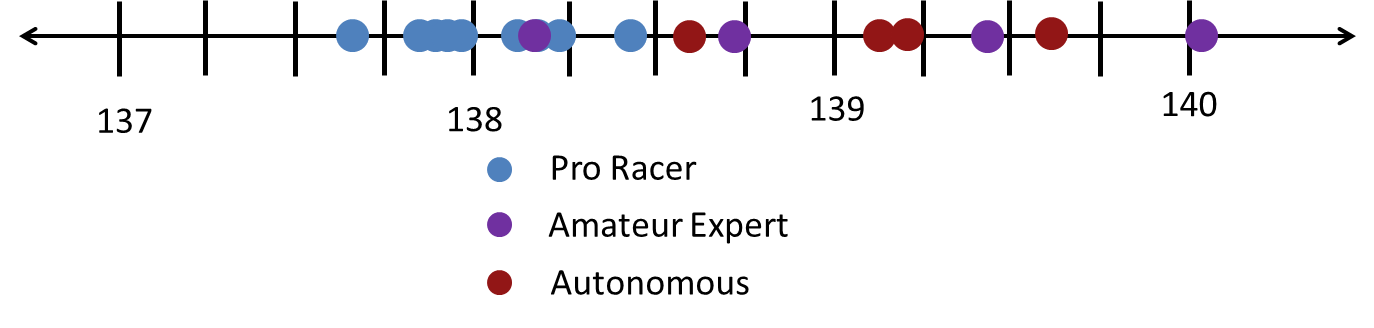
\includegraphics[width=.9\fullwidth]{expLT.png}
\caption{Experimentally recorded lap times (in seconds).}
\label{fig:expLT}
\end{figure}

While the lap times from the autonomous driver are comparable to the amateur expert, they are about a second behind on average from the professional
human driver. There are several ways to analyze why this difference arises, but a simple insight that makes the case for learning algorithms comes
from viewing the trajectory tracking performance and friction utilization of the controller, shown in Fig.~\ref{fig:expErrors}.

\begin{figure}
\centering
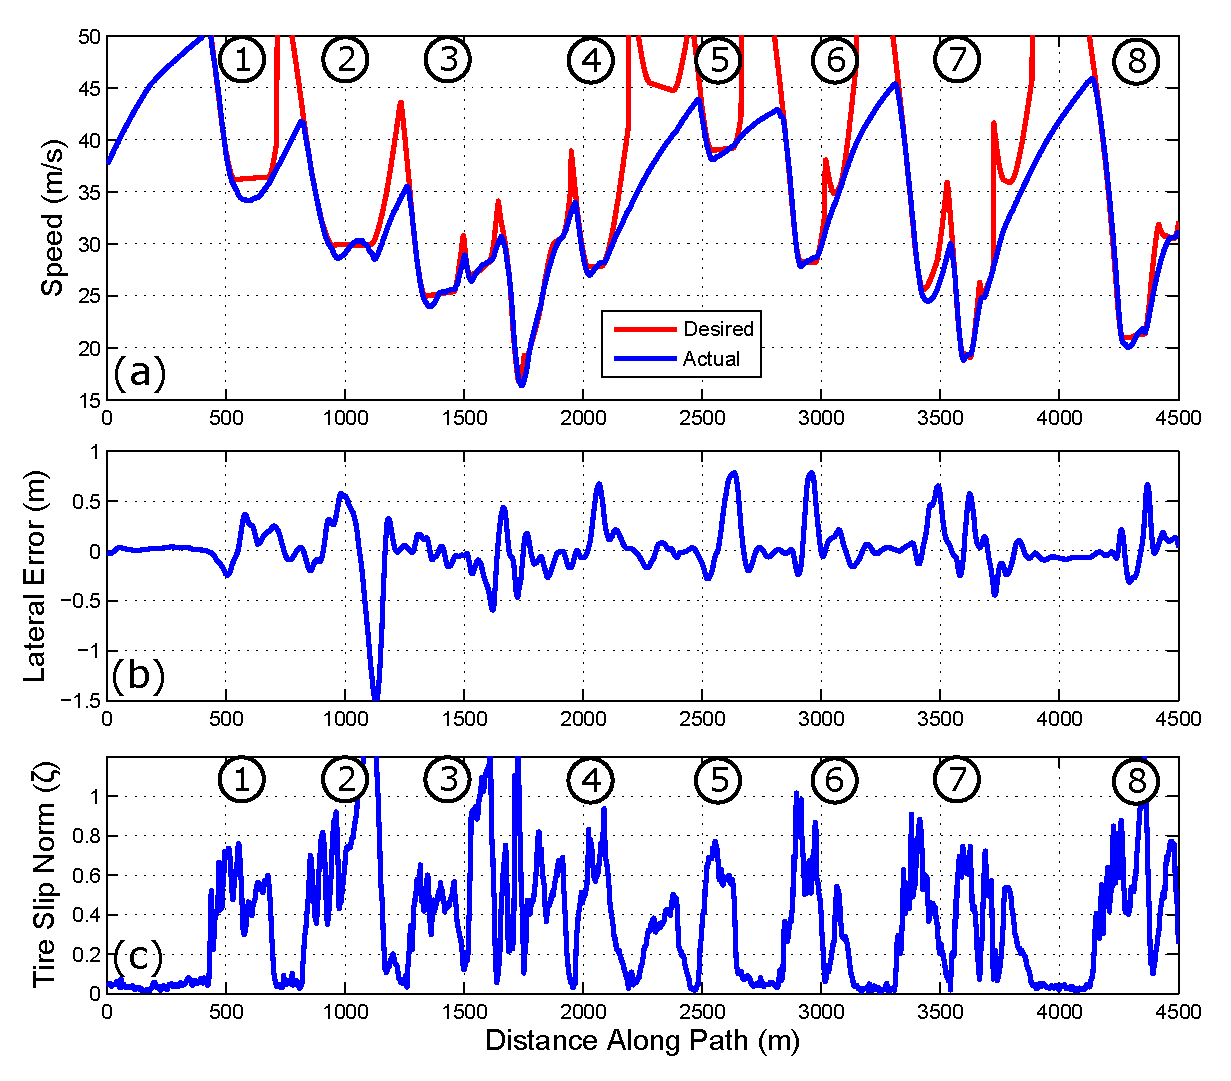
\includegraphics[width=\fullwidth]{expErrors.eps}
\caption{Controller tracking performance and tire slip norm on a test run at the limits of handling ($\mu =$ 0.95).(a) Desired
vs actual speed of the vehicle. (b) Lateral tracking error and (c) tire slip norm as a function of distance along the path.}
\label{fig:expErrors}
\end{figure}

One of the issues shown in Fig.~\ref{fig:expErrors} is the relatively poor controller tracking on a few sections of the race track. While
this is probably less significant for the lateral speed tracking (sections \circled{2}, \circled{4} - \circled{7}), failing to drive as fast as the trajectory plans (sections \circled{1}, \circled{2}, \circled{7}) results directly in a loss 
of lap time. The speed and lateral path tracking will be improved in this chapter with the addition of iterative learning control
(ILC) algorithms. 

The second issue shown in Fig.~\ref{fig:expErrors} is the inconsistent usage of the tire friction capacity, as judged by the tire slip norm metric.
The tire slip norm, formalized in \cite{mickthesis}, is given by $\zeta$:

\begin{equation}
\label{eq:zeta}
\zeta = \sqrt{\left(\dfrac{\alpha}{\alpha_{p}}\right)^2 + \left(\dfrac{\sigma}{\sigma_p}\right)^2}
\end{equation}

Where $\sigma$ and $\alpha$ are the longitudinal and lateral tire slip for a given tire, and $\sigma_p$ and $\alpha_p$ are empirically
determined \textit{peak slip} values resulting in maximum longitudinal and lateral tire force generation. As a result, $\zeta < 1 $ corresponds to the tires having
excess force generation capacity, while $\zeta > 1$ corresponds to tire saturation. There is technically a $\zeta$ value for each tire, but the maximum
$\zeta$ over all four tires is typically used for conservatism. 

Fig.~\ref{fig:expErrors} shows inconsistent usage of tire friction across many turns. On some turns (sections \circled{2} and \circled{8}), the vehicle significantly exceeds
the limits of handling, and the car's stability control systems kick in to regain control, slowing the car down in the process. On other turns (sections \circled{3}, \circled{5}, and \circled{7}),
the vehicle uses only a portion of the available tire force, indicating the vehicle can actually drive with higher acceleration on the next lap. 
Learning from prior runs to find the optimal acceleration (or $\mu$ parameter) for each part of the track will be accomplished in the next chapter via a search algorithm. 

\subsubsection{Iterative Learning Control}

Iterative learning control (ILC) is based on the notion that the performance of a system that executes the
\textit{same task} multiple times can be improved by learning from previous executions (trials, iterations, or in our case, laps of racing) \cite{bristow}.
On every iteration, a control signal is applied to a system in order to follow an ideal, unchanging ``reference trajectory". 
The tracking error for that iteration is recorded, and a learning algorithm is applied to improve the control signal and achieve
more accurate system performance on the next iteration. There are a variety of learning algorithms used, but most attempt to correct the tracking
error by using a model of the system to determine the augmentation to apply to the prior control signal. This process is repeated until the reference tracking performance becomes satisfactory.
As noted by Bristow et al., this approach is analogous to how a basketball player shooting a free throw from a fixed position can improve her ability to
score by practicing the shot repeatedly, making adjustments to her shooting motion based on observations of the ball's trajectory \cite{bristow}.

Inspired by a series of papers published in 1984 \cite{arimoto}\cite{craig}\cite{kawamura}, iterative learning control has become increasingly widespread. Because
iterative learning control works best when learning to follow the same reference trajectory under the same ambient conditions, the most common applications
of ILC are in the field of automated manufacturing. Notable examples include CNC machining \cite{kimdi}, industrial robotics \cite{freeman}\cite{hladowski}, piezolectric stage
positioning \cite{huang}, motor control \cite{mohammad}, and microdeposition \cite{hoelzle}. However, the rise of automated systems outside
factory environments has led to important applications of ILC for ground and air robotics. In 2006, Chen and Moore \cite{chen} proposed
 a simple iterative learning scheme in 2006 to improve path-following of a ground vehicle with omni-directional wheels. In 2011, Purwin and Andrea synthesized
 an iterative controller using least-squares methods to aggressively maneuver a quadrotor
 unmanned aerial vehicle (UAV) from one state to another \cite{purwin}. As a novel step, the authors then generalized the experience learned
 from the iterative learning control in order to tune the parameters of the UAV model. In 2013, Sun et al. \cite{sun}
 proposed an iterative learning controller for speed regulation of high-speed trains. Given the high safety requirements of fast trains, the algorithm
heavily penalized train overspeeding and enabled the trains to learn how to maintain a safe following distance. 

Due to the nature of automotive racing, iterative learning control techniques are a promising method to gradually
eliminate the trajectory tracking errors described in Fig.~\ref{fig:expErrors}. For this application of ILC, the 
repetitive trials are laps of racing, and the reference trajectory is the optimal speed profile and curvature profile from Chapter 3. This chapter will 
present adaptations
of two established ILC methods (proportional-derivative and quadratically optimal) for use in the Audi TTS racing system. Section \ref{sec:ch4dsm} presents
both coupled and decoupled models of the vehicle lateral and longitudinal dynamics. These models are converted from state-space representations to \textit{lifted domain}
representations required for iterative learning control in \S \ref{sec:liftedD}, and the proportional-derivative and quadratically optimal ILC algorithms are presented
in \S \ref{sec:pdcontroller} and \S \ref{sec:qopt}. Section \ref{sec:simres} presents simulated results of the ILC algorithms for a sample vehicle trajectory, and finally,
experimental results showing a gradual reduction of trajectory-following errors is presented in \S \ref{sec:ch4ExpRes}.

\section{Dynamic System Model}
\label{sec:ch4dsm}
The ILC algorithms we consider require the closed-loop system dynamics to be (a) stable to any disturbance input, and (b) expressible as an \textit{affine} discrete dynamical system.
In our case, we have two subsystems: the steering controller and the longitudinal speed control. Stability of the steering controller
under lanekeeping feedback was shown in the linear case by \cite{rossetter2002} and in the saturated case by \cite{talvala}, and was also 
discussed in Chapter 2. Similar analyses can be considered to show the stability of the simple proportional speed-following controller.

The more difficult task is expressing the dynamics of the two subsystems using an affine model, given the tendency for the vehicle tires
to saturate at the limits. Chapter 2 presented the  lateral vehicle dynamics obtained by neglecting longitudinal forces. However, since we are 
modifying both the longitudinal force $F_x$ and steer input $\delta$ on each iteration, it may be important to account for the coupled
lateral/longitudinal dynamics of the vehicle. Nonlinear, coupled equations of motion are provided in (\ref{eq:fullNL})-(\ref{eq:fullNL2}):

\begin{align}
\label{eq:fullNL}
	\dfrac{de}{dt} &= \left(v+U^\mathrm{des}_x(s)\right)(\beta + \Delta\Psi) \\
	\dfrac{dv}{dt} &= \left(v+U^\mathrm{des}_x(s)\right)\beta r + \frac{F_x}{m} - \frac{F_\mathrm{yf}(\alpha_\mathrm{f},F_x)\delta}{m}\\
	\dfrac{d\beta}{dt} &= \frac{F_\mathrm{yf}(\alpha_\mathrm{f}, F_x) + F_\mathrm{yr}(\alpha_\mathrm{r},F_x)}{m\left(v + U^\mathrm{des}_x(s)\right) - r} \\
	\dfrac{dr}{dt}     &= \frac{aF_\mathrm{yf}(\alpha_\mathrm{f}, F_x) - bF_\mathrm{yr}(\alpha_\mathrm{r}, F_x)}{I_z} \\
	\dfrac{d\Delta\Psi}{dt} &= r \label{eq:fullNL2}
\end{align}
The system dynamics presented in (\ref{eq:fullNL}) have five states, the original four from Chapter 2 and a new state $v$, the
 speed tracking error of the system defined by:
\begin{equation}
v = U_x - U^\mathrm{des}_x
\end{equation}
The two inputs to the nonlinear system are the steering angle $\delta$ and longitudinal force $F_x$. In reality,
the true longitudinal input is a brake pressure or throttle input, but longitudinal force control is assumed for simplicity.
The potential for coupling between the subsystems is apparent from (\ref{eq:fullNL}), not only directly from the state
equations but also due to the complex nature of tire force generation at the handling limits. As shown in Fig.~\ref{fig:coupledTires}, as longitudinal
force $F_x$ is distributed across the tires, the available lateral force decreases. At the limits of handling, this
\textit{derating} of the lateral force may become significant. As a result, we now model $F_y$ as a function
of both lateral tire slip $\alpha$ and the applied longitudinal force $F_x$, using a modified form of the Fiala equation
presented in Chapter 2 \cite{rami}. Recall that the front and rear tire slip are themselves functions of the vehicle state and are
given by: 

\begin{subequations}
\begin{align}
	\alpha_\mathrm{f} &= \beta + \frac{ar}{U_x} - \delta\\
	\alpha_\mathrm{r} &= \beta - \frac{br}{U_x}
\end{align}
\end{subequations}

\begin{figure}[tb]
\centering
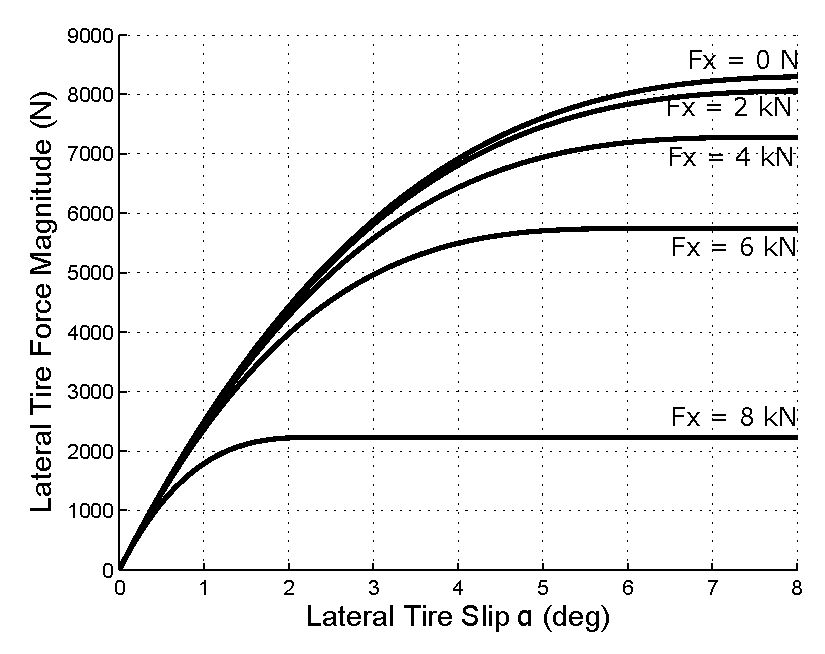
\includegraphics[width=.8\fullwidth]{tirecurves.eps}
\caption{Lateral tire force curve as a function of longitudinal force $F_x$ and lateral tire slip $\alpha$.}
\label{fig:coupledTires}
\end{figure} 

The next step is to break up the control inputs into the closed-loop feedback term and the \textit{learned} component that is
modified on every lap by the ILC algorithm:
\begin{align}
\label{eqn:splitTerms}
F_x &= F^{\mathrm{FB}}_x + F^L_x\\
    &= -K_xv + F^L_x\\
\delta &= \delta_{\mathrm{FB}} + \delta_L\\
\delta &= -k_p(e + x_\mathrm{LA}\Delta\Psi) + \delta_L
\end{align}
where $K_x$ is the proportional speed tracking gain and $k_p$ and $x_\mathrm{LA}$ are the lookahead gains discussed in Chapter 2. Note
that (\ref{eqn:splitTerms}) is similar to a feedback-feedforward control formulation. In fact, iterative learning control achieves
near-perfect reference tracking by refining the \textit{feedforward} control input to account for unmodeled dynamics and repeating disturbances that
affect the closed-loop controller performance. 

The closed loop system dynamics are now given by: 
\begin{align}
\label{eq:fullNLCL}	
	\frac{de}{dt} &= \left(v+U^\mathrm{des}_x(s)\right)(\beta + \Delta\Psi) \\
	\frac{dv}{dt} &= \left(v+U^\mathrm{des}_x(s)\right)\beta r + \frac{-K_xv + F^L_x}{m} - \frac{F_\mathrm{yf}(\alpha_F,F_x)-k_p(e + x_{LA}\Delta\Psi) + \delta_L}{m}\\
	\frac{d\beta}{dt} &= \frac{F_\mathrm{yf}(\alpha_\mathrm{f}, F_x) + F_\mathrm{yr}(\alpha_\mathrm{f},F_x)}{m\left(v + U^\mathrm{des}_x(s)\right) - r} \\
	\frac{dr}{dt}     &= \frac{aF_\mathrm{yf}(\alpha_\mathrm{f}, F_x) - bF_\mathrm{yr}(\alpha_\mathrm{r}, F_x)}{I_z} \\
	\frac{d\Delta\Psi}{dt} &= r
\end{align}
The nonlinear closed-loop dynamics must be converted into an affine, discrete-time dynamical system to apply conventional iterative learning
control algorithms. In our case, we have two system outputs ($y = [e \hspace{2mm} v]^T$) that are measured and two input signals to learn ($u = [\delta_L \hspace{2mm} F^L_x]^T$). 
Since we run the iterative learning control algorithm after seeing a trial of data, we can approximate
the dynamics in (\ref{eq:fullNLCL}) by linearizing about the observed states and inputs $x_o, u_o$ from the first lap. The affine model is therefore given by: 
 \begin{align}
 \label{eq:ssMAT}
 \begin{bmatrix} \dot{e} \\ \dot{\beta} \\ \dot{r} \\ \dot{\Delta\Psi} \\ \dot{v}\end{bmatrix} &= \begin{bmatrix} A(t) \end{bmatrix} \begin{bmatrix} e \\ \beta \\ r \\ \Delta\Psi \\ v \end{bmatrix} + \begin{bmatrix} B(t) \end{bmatrix} \begin{bmatrix} \delta_L \\ F^L_x \end{bmatrix} + d(t) \\
 \begin{bmatrix} \dot{e} \\ \dot{v} \end{bmatrix}  &= \begin{bmatrix} 1 & 0 & 0 & 0 & 0 \\ 0 & 0 & 0 & 0 & 1 \end{bmatrix} x
 \end{align}
 
 The time-varying state space matrices  where $A(t)$ and $B(t)$ are given by Jacobian linearizations of the closed loop nonlinear dynamics $f(x)$ (\ref{eq:fullNLCL}) about the observed states and inputs $x_o(t), u_o(t)$ from the last trial:
 \begin{align}
 \label{eq:C4nl}
 \begin{bmatrix} A(t) \end{bmatrix} &= \frac{\partial{f}}{\partial{x}}\Big|_{x_o(t)} \\
 \begin{bmatrix} B(t) \end{bmatrix} &= \frac{\partial{f}}{\partial{u}}\Big|_{u_o(t)}
 \end{align}
 While this multiple-input, multiple-output (MIMO) model captures the coupled behavior of the longitudinal and lateral inputs, it is tedious to compute,
 either numerically or analytically. For the case where the longitudinal and lateral inputs are decoupled, we obtain the same Chapter 2 linear state equations for the lateral
 dynamics: 
\begin{subequations}
\label{eq:bmC4}
\begin{align}
	\dot{\beta} &= \frac{F_\mathrm{yf}+F_\mathrm{yr}}{mU_x} - r \qquad \dot{r} = \frac{aF_\mathrm{yf} - bF_\mathrm{yr}}{I_z} \label{bm1} \\
	\dot{e} &= U_x (\beta + \Delta\Psi) \qquad \Delta\dot{\Psi} = r - U_x\kappa \label{eq:bm2} 
\end{align}
\end{subequations} 
and the following first order equation for the longitudinal dynamics, assuming a simple point mass model with proportional
speed tracking feedback:
\begin{equation}
\dot{v} = \frac{-K_xv + F^L_x}{m}
\end{equation}
The resulting state matrices $A(t)$ and $B(t)$ for (\ref{eq:ssMAT}) are then simply block diagonal matrices consisting of the
linearized lateral dynamics from Chapter 3 and the first order longitudinal dynamics:

\begin{align}
\label{eqn:C4dyn}
 A(t)  &= \begin{bmatrix}
  0 & U_x(t) & 0 & U_x(t) & 0\\ 
  0 & 0 & 1 & 0 & 0 \\ 
  \frac{-ak_\mathrm{p} \tilde{C}_\mathrm{f}(t)}{I_\mathrm{z}}  & \frac{-ak_\mathrm{p}x_\mathrm{LA}\tilde{C}_\mathrm{f}(t)}{I_\mathrm{z}}  & \frac{-a^2\tilde{C}_\mathrm{f}(t)-b^2\tilde{C}_\mathrm{r}(t)}{U_x(t)I_\mathrm{z}} & \frac{b\tilde{C}_\mathrm{r}(t) - a\tilde{C}_\mathrm{f}(t)}{I_\mathrm{z}} & 0 \\
  \frac{-k_\mathrm{p}\tilde{C}_\mathrm{f}(t)}{mU_x(t)}  & \frac{-k_\mathrm{p}x_\mathrm{LA}\tilde{C}_\mathrm{f}(t)}{mU_x(t)}  & \frac{b\tilde{C}_\mathrm{r}(t)-a\tilde{C}_\mathrm{f}(t)}{mU_x(t)^2}-1 & \frac{-\tilde{C}_\mathrm{f}(t) - \tilde{C}_\mathrm{r}(t)}{mU_x(t)} & 0 \\
  0 & 0 & 0 & 0 & -K_x 
  \end{bmatrix} \\
B(t) &=\begin{bmatrix} 0 & 0 \\	 	0 & 0 		\\ 		\frac{a \tilde{C}_\mathrm{f}(t)}{I_\mathrm{z}} & 0 		\\ 		\frac{\tilde{C}_\mathrm{f}(t)}{mU_x(t)} & 0 		\\ 0 & 1 \end{bmatrix} 
\end{align}
The affine term $d(t)$ is given by: 
\begin{align}
d(t) = \left[\begin{matrix} 0 \\
               -\kappa(t) U_x(t) \\ 
			    \frac{a\tilde{C}_\mathrm{f}(t)\tilde{\alpha}_\mathrm{f}(t) - b\tilde{C}_\mathrm{r}(t)\tilde{\alpha}_\mathrm{r}(t) + a\tilde{F}_\mathrm{yf}(t) - b\tilde{F}_\mathrm{yr}(t)}{I_z}\\
				\frac{\tilde{C}_\mathrm{f}(t)\tilde{\alpha}_\mathrm{f}(t) + \tilde{C}_\mathrm{r}(t)\tilde{\alpha}_\mathrm{r}(t) + \tilde{F}_\mathrm{yf}(t) + \tilde{F}_\mathrm{yr}(t)}{mU_x(t)}\\
				0 \\
				0
				\end{matrix}\right]
\end{align}
While (\ref{eqn:C4dyn}) is written as a MIMO system for compactness, assuming decoupled lateral and longitudinal 
dynamics provides two single-input, single-output (SISO) systems. 

\newpage
\section{Lifted Domain Representation and ILC \newline Problem Statement}
\label{sec:liftedD}
Whether the coupled (\ref{eq:C4nl}) or decoupled (\ref{eqn:C4dyn}) dynamics are assumed, the
final modeling step is to apply standard discretization techniques to obtain dynamics in the following form:
\begin{align}
\label{C4ad}
x_{k+1} &= A_kx_k + B_ku_k + d_k \\
y_{k}   &= Cx_k
\end{align}
For a given lap of racing $j$, sensor measurements provide $N$ observations of both the lateral path deviation $e$ and longitudinal
speed tracking error $v$. These measurements can be stacked into a 2$N \times 1$ array: 
\begin{equation}
\mathbf{e}_j = \begin{bmatrix} e_1 & \hdots & e_N & v_1 & \hdots & v_N \end{bmatrix}^T
\end{equation} 
These measurement errors are related to the learned control inputs $\delta^L$ and $F^L_x$ as follows: 
\begin{align}
\label{eq:liftedDomain}
\mathbf{e}_j &= P\mathbf{u}^L_j + \mathbf{w} \\
\mathbf{u}^L_j &= \begin{bmatrix} \delta^L_1 & \hdots & \delta^L_N & F^L_{x1} & \hdots & F^L_{xN} \end{bmatrix}^T
\end{align}
The system dynamics modeled in the previous section are represented by the \textit{lifted-domain} dynamics matrix $P$,
which is $\mathrm{2}N \times \mathrm{2}N$ and given by:
\begin{equation}
\label{eq:C4bm}
P=\left[
\begin{array}{c|c}
P_{e\delta} & P_{eF} \\ \hline
P_{v\delta} & P_{vF} 
\end{array}\right]
\end{equation}
Where each submatrix in (\ref{eq:C4bm}) is $N \times N$ and represents the lifted-domain dynamics from a given input to a given output. 
Individual terms of the sub-matrices are given by:

\begin{equation}
\label{eq:how2Lift}
p_{lk} = \begin{cases} 0 &\mbox{if } l < k \\ 
C_yB_u(k) & \mbox{if } l = k \\
C_yA(l)A(l-1)\cdots A(k)B_u(k) &\mbox{if } l > k \end{cases}
\end{equation} 
Where $C_y$ is the row of $C$ in (\ref{C4ad}) corresponding to the desired output and $B_u$ the column of $B$ in (\ref{C4ad})
corresponding to the desired input. Note that
for the case of uncoupled lateral and longitudinal dynamics, the off-diagonal sub-matrices of $P$ are $[0]$ since we have
two SISO systems. The term $\mathbf{w}$ in (\ref{eq:liftedDomain}) is the unknown disturbance. Iterative
learning control relies on the assumption that this disturbance is the underlying cause of the observed errors $\mathbf{e}_j$, and that 
the disturbance, while unknown, is constant from lap to lap.

Given the error signal $\mathbf{e}_j$ for a given lap $j$, the iterative learning problem is to find the inputs $\mathbf{u}_{j+1}$ that
will cancel out the tracking error on the next lap. The learned inputs are then applied, the observed error $\mathbf{e}_{j+1}$ is recorded,
and the process is repeated until the tracking error falls to a desired level. There is a wide body of literature on methods to determine $\mathbf{u}_{j+1}$ given $P$ and $\mathbf{e}_j$, but this dissertation will
investigate the most common approach. We compute the ILC input for the next lap with the following formulation:

\begin{align}
 \label{eqn:ctrlLaw}
 \mathbf{u}^L_{j\!+\!1} = Q(\mathbf{u}^L_j - L\mathbf{e}_j)
\end{align}
where $Q$ is the $2N \times 2N$ \textit{filter} matrix, and $L$ is the $2N \times 2N$ \textit{learning} matrix. 
In the following two sections, the
matrices $Q$ and $L$ will be obtained by designing a proportional-derivative (PD) iterative learning controller as well as a quadratically
optimal (Q-ILC) learning controller.

\newpage
\section{Proportional-Derivative Controller}
\label{sec:pdcontroller}

The proportional-derivative ILC computes the steering $\delta^L$ and force $F^L$ correction for the current lap $j$ based on the error and 
error derivative at the same time index $k$ from the previous lap:
\begin{align}
	\label{eq:PDlaw}
	\delta^L_{j}(k) &= \delta^L_{j\!-\!1}(k) - k_{p\delta}e_{j\!-\!1}(k) - k_{d\delta}(e_{j\!-\!1}(k) - e_{j\!-\!1}(k-1))\\
	    F^L_{j}(k) &=  F^L_{j-1}(k) - k_{pF}v_{j\!-\!1}(k) - k_{dF}(v_{j\!-\!1}(k) - v_{j\!-\!1}(k-1))
\end{align}
where $k_{p\delta}$ and $k_{pF}$ are proportional gains and $k_{d\delta}$ and $k_{dF}$ are derivative gains. In the lifted domain representation from (\ref{eqn:ctrlLaw}), the resulting learning matrix $L$ is given by
\begin{equation}
	L = \begin{bmatrix} 		-(k_{p\delta}+k_{d\delta}) &          &  0                            & 0 & \hdots & 0 \\ 
									   k_{d\delta}                     &  \ddots  &                               & \vdots & \ddots & \vdots\\ 
									   0                       &   k_{d\delta}    &    -(k_{p\delta}+k_{d\delta}) & 0 & \hdots & 0 \\
						               0 & \hdots & 0 & -(k_{pF}+k_{dF}) &          &  0\\
									   \vdots & \ddots & \vdots & k_{dF} &  \ddots  &                               &\\
									   0 & \hdots & 0  & 0 & k_{dF} & -(k_{pF} + k_{dF}) \\			
			\end{bmatrix}
\end{equation}
 
 The PD equation (\ref{eq:PDlaw}) determines $\delta^L$ only using lateral path deviation $e$ and $F^L_x$ using only the speed tracking error $v$. Since
 we have formulated the problem as a MIMO system, it is possible to generalize and have both inputs depend on both outputs, but this is not considered for 
 simplicity of gain selection. The filter matrix $Q$ is obtained by taking any filter transfer function and converting into the lifted domain via (\ref{eq:how2Lift}).
 An important design consideration in choosing the two $k_p$ and $k_d$ gains is avoiding a poor lap-to-lap
``transient" response, where the path tracking error increases rapidly over the first several laps before
eventually decreasing to a converged error response $e_\infty$. This is a commonly encountered design requirement
for ILC systems, and can be solved by ensuring the following \textit{monotonic convergence} condition is met \cite{bristow}:

\begin{equation}
	\gamma \triangleq \bar{\sigma}(PQ(I-LP)P^{-1}) < 1
	\label{eq:MS}
\end{equation}
where $\bar{\sigma}$ is the maximum singular value. In this case, the value of $\gamma$ provides an upper bound on the change
 in the tracking error norm from lap to lap, i.e. 
 
\begin{equation}
	||\mathbf{e}_\infty - \mathbf{e}_{j+1}||_2 \leq \gamma ||\mathbf{e}_\infty-\mathbf{e}_j||_2
\end{equation}

Fig.~\ref{fig:stabPlot} shows values of $\gamma$ for both an unfiltered PD controller ($Q = I$), and for a PD controller with a 2 Hz, first order low pass filter. The $\gamma$ values are plotted as a
contour map against the controller gains $k_{p\delta}$ and $k_{d\delta}$. Addition of the low-pass filter
assists with monotonic stability by removing oscillations in the control input generated when trying to remove small reference tracking
errors after several iterations. Since the filtering occurs when generating a control signal for the next lap, the filter $Q$ can be zero-phase. 
The plot shown in Fig.~\ref{fig:stabPlot} is for the steering ILC design only, but the same analysis is possible for the longitudinal
ILC design as well. The stability analysis in Fig.~\ref{fig:stabPlot} assumes the $P$ 
matrix is constant for all iterations and is generated assuming decoupled vehicle dynamics
 for a straight-line trajectory at a constant speed of 20 m/s. Because the $P$ matrix in general can change from iteration to iteration and will also
 change depending on the trajectory, making a general assertion or proof about stability of the iterative learning controller is difficult. 

\begin{figure}[tb]
\centering
\includegraphics[width=.7\fullwidth]{MonotonicStability.png}
\caption[Values of convergence bound $\gamma$ vs. $k_{p\delta}$ and $k_{d\delta}$ for PD iterative learning controller]{Values of convergence bound $\gamma$ vs. $k_{p\delta}$ and $k_{d\delta}$ for PD iterative learning controller with (top) no filtering and (bottom) with a 2 Hz low-pass filter. Lower values of $\gamma$ correspond to faster convergence.
Shaded regions correspond to gains that result in system monotonic stability. }
\label{fig:stabPlot}
\end{figure}


\section{Quadratically Optimal Controller}\label{sec:controller}
\label{sec:qopt}
An alternate approach to determining the learned steering and longitudinal force input is to minimize a quadratic cost function for the next lap:

\begin{align}
J_{j\!+\!1} = \textbf{e}_{j\!+\!1}^TT\textbf{e}_{j\!+\!1} + \textbf{u}^T_{j\!+\!1} R \textbf{u}^T_{j\!+\!1}+\Delta_{j\!+\!1}^TS\Delta_{j\!+\!1}
\label{eq:QILC}
\end{align}
where $\Delta_{j\!+\!1} = \mathbf{u}^L_{j\!+\!1} - \mathbf{u}^L_j$ and the $2N \times 2N$ matrices $T$, $R$, and $S$ are weighting matrices, each given
by a scalar multiplied by the identity matrix for simplicity.
This formulation allows the control designer to weight the competing objectives of minimizing the tracking errors $e$ and $v$, control effort $|\delta^L|$ and $|F^L_x|$, and change in the control signal from lap to lap.
While constraints can be added to the optimization problem, the unconstrained problem in (\ref{eq:QILC}) can be solved analytically \cite{bristow2008} to obtain desired controller and filter matrices:

\begin{subequations}
\label{eq:analSol}
\begin{align}
	Q &= (P^TTP + R + S)^{-1}(P^TTP + S)\\
	L &= (P^TTP + S)^{-1}P^TTP(T^{1/2}P)^{-1}T^{1/2}
\end{align}
\end{subequations}

An advantage of the quadratically optimal control design over the simple PD controller is that the controller matrices $Q$ and $L$ take the linearized, time-varying dynamics $P$ into account. 
This allows the iterative learning algorithm
to take into account changes in the steering dynamics due to changes in vehicle velocity.
Furthermore, if the fully coupled dynamics (\ref{eq:C4nl}) are used, the iterative learning algorithm also accounts for the
second-order effect of steering on the longitudinal dynamics and longitudinal force application on the lateral dynamics. 
 However, a disadvantage is that computing $\mathbf{\delta}^L$ in (\ref{eqn:ctrlLaw}) requires matrix multiplications with
the typically dense matrices $Q$ and $L$ for every lap, which can be computationally expensive for fast sampling rates. 

\section{Simulated Results}
\label{sec:simres}

To test the feasibility of the PD and Q-ILC learning algorithms, the vehicle tracking performance over multiple laps is
simulated using the path curvature and speed profiles shown in Fig.~\ref{fig:simSetup}. To test the performance
of the controller at varying accelerations, four speed profiles are tested. Each profile is
generated with a different level of peak combined longitudinal/lateral acceleration, ranging from 5 $\mathrm{m/s^2}$ (below the limits)
up to 9.5 $\mathrm{m/s^2}$ (close to exceeding the limits). For accurate results, simulations were conducted using numerical integration with
 fully nonlinear equations of motion (\ref{eq:fullNL})-(\ref{eq:fullNL2}) and coupled lateral/longitudinal dynamics \cite{rami}.

\begin{figure}[bh]
\centering
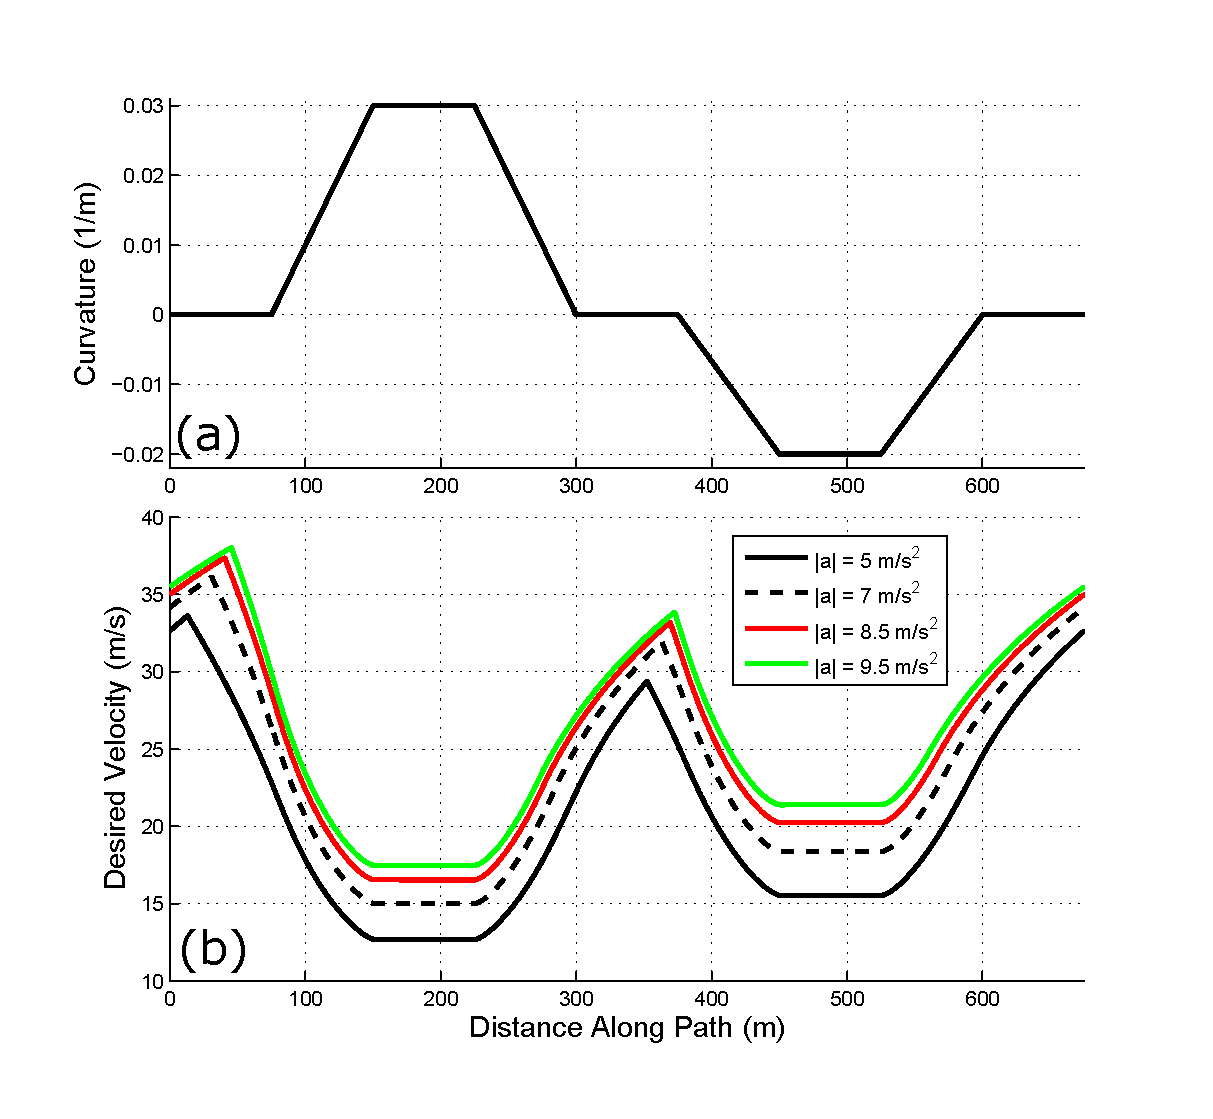
\includegraphics[width= .88\fullwidth]{simSetup.eps}
\caption[Curvature profile used for ILC simulation.]{ (a) Curvature profile used for ILC simulation. (b) Velocity profiles generated for four different levels of longitudinal/lateral acceleration. }
\label{fig:simSetup}
\end{figure}

Simulated results for the root-mean-square (RMS) lateral path deviation is shown in Fig.~\ref{fig:simRes1}. The results
show the change in RMS error as the number of ILC iterations increase. Three different ILC controllers are tested. 
The first controller is the simple PD controller
with low-pass filter (\ref{eq:PDlaw}), and the second controller is the quadratically optimal ILC algorithm (\ref{eq:analSol}) assuming fully coupled dynamics (\ref{eq:C4nl}) in the plant
matrix $P$ (i.e. the full MIMO system).
The third controller is also the quadratically optimal ILC algorithm, but the $P$ matrix used in the optimization
assumes decoupled dynamics (\ref{eqn:C4dyn}) and therefore solves the lateral and longitudinal SISO problems separately. 

\begin{figure}[h!]
\centering
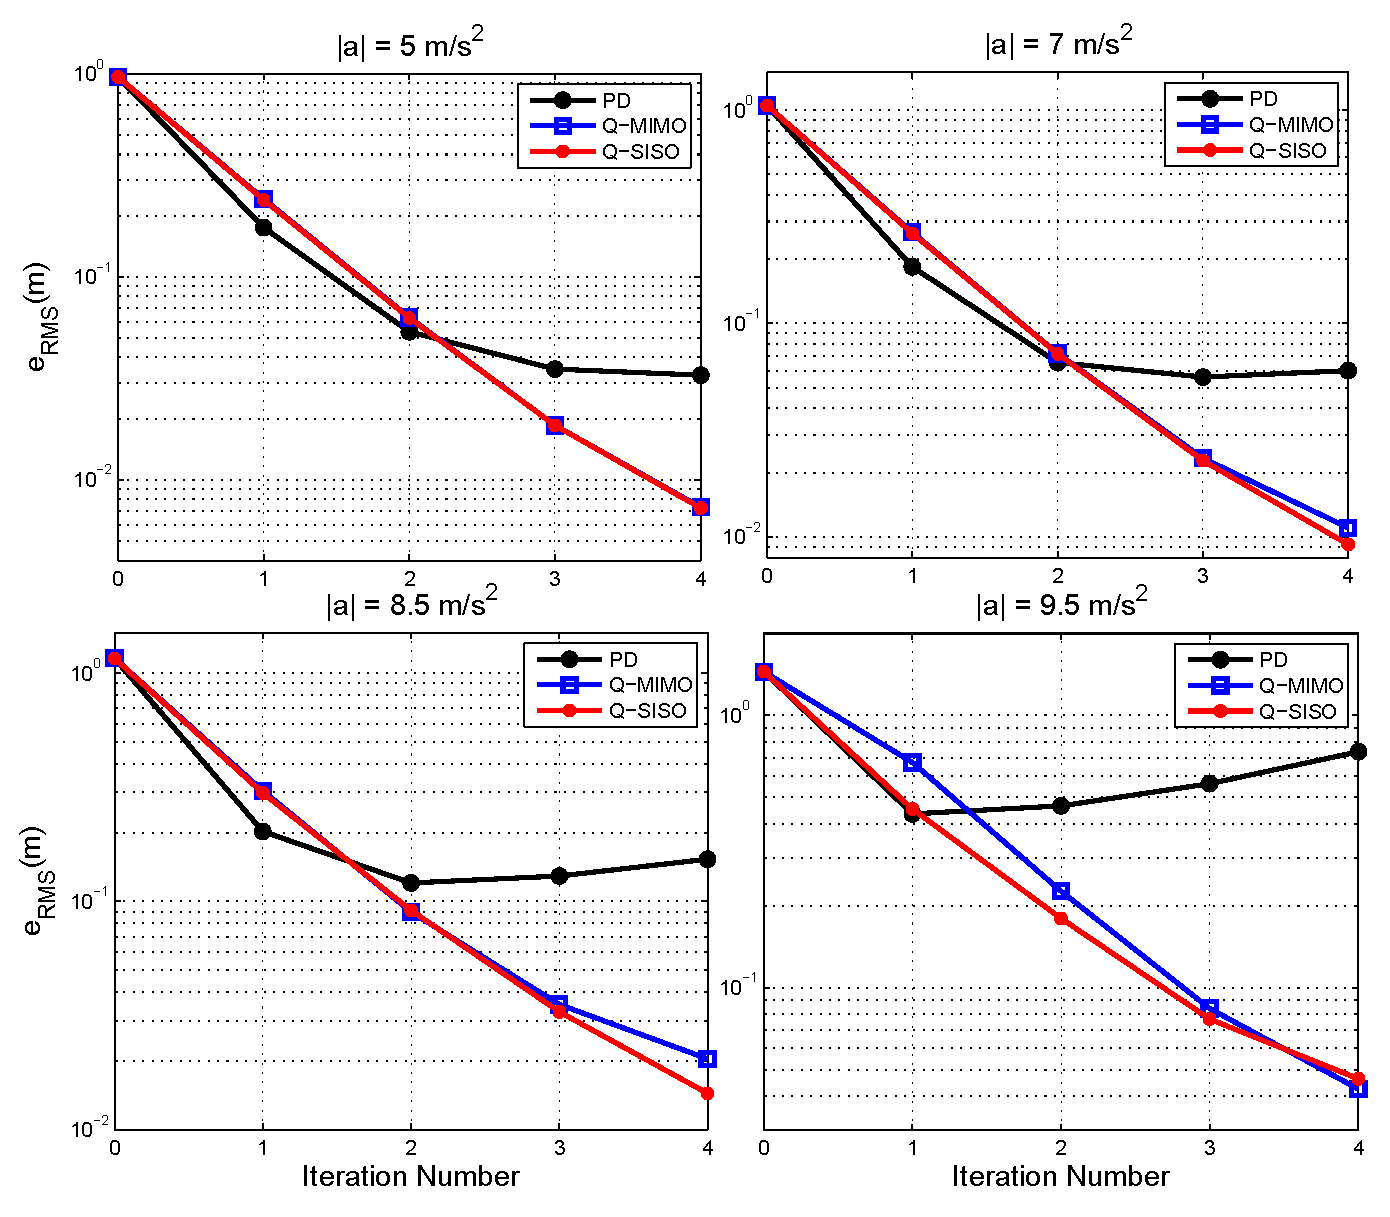
\includegraphics[width=.92\fullwidth]{simRes1.eps}
\caption[Simulated results for root-mean-square path tracking error at several values of vehicle acceleration]{Simulated results for root-mean-square path tracking error at several values of vehicle acceleration, with $T = R = I$ and $S = \mathrm{100} I$.
Results are plotted on a log scale.}
\label{fig:simRes1}
\end{figure}

Fig.~\ref{fig:simRes1} shows that both quadratically optimal ILC algorithms exponentially reduce the lateral
path tracking error as the number of learning iterations is increased. Overall, the RMS lateral tracking performance is
better at lower vehicle accelerations. This is unsurprising for two reasons. In Chapter 2, we discovered that lateral path deviation in 
general increases for the lookahead steering feedback at higher accelerations. Second, our estimate of the vehicle dynamics contained in $P$
is based on linearization, and the vehicle dynamics at lower accelerations are mostly linear.

Fig.~\ref{fig:simRes2} shows the same results as Fig.~\ref{fig:simRes1}, but for the speed tracking performance. 
The overall trends are very similar. In both plots, there is very little difference between the coupled MIMO formulation and decoupled SISO 
formulation at low accelerations. This is expected, as the longitudinal and lateral dynamics are independent when the vehicle tires are not saturated.
At higher accelerations, there are small differences, but the overall RMS errors are still quite similar. A reason for this is the
nature of the speed profiles in Fig.~\ref{fig:simSetup}. The vehicle spends the majority of time either fully braking/accelerating or
turning at a constant velocity. There are only a few small transient regions where the vehicle needs significant amounts of both 
lateral and longitudinal acceleration. As a result, the need to account for the coupled dynamics may not be important in practice, especially
given the larger computation time needed when $P$ is dense and not block-diagonal.     

\begin{figure}[tb]
\centering
\includegraphics[width=\fullwidth]{simRes2.eps}
\caption[Simulated results for root-mean-square speed tracking error $v$ at several values of vehicle acceleration.]{Simulated results for root-mean-square speed tracking error $v$ at several values of vehicle acceleration, with $T = I$, $R = 0$, and $S = \mathrm{1e-7} I$.
Results are plotted on a log scale.}
\label{fig:simRes2}
\end{figure}

A final comment is that the proportional-derivative ILC algorithm performs relatively poorly. At low accelerations, the
speed and path tracking performance both improve initially, but fail to improve after the second learning iteration. At high
lateral and longitudinal accelerations, the tracking performance becomes even worse for the steering ILC in Fig.~\ref{fig:simRes1}.  
This is unsurprising given that the linearized plant dynamics $P$ are not explicitly accounted for in the selection of the PD gains. 
While the point mass model for the longitudinal dynamics is a relatively simple first order model, the lateral dynamics 
are fourth order and highly speed dependent. A simple PD approach for learning control is likely insufficient at the limits of handling
without a more sophisticated set of PD gains for different vehicle speeds.

\section{Experimental Results}
\label{sec:ch4ExpRes}

Experimental data for iterative learning control was collected over four laps at Thunderhill Raceway with the autonomous Audi TTS
setup described in Chapters 2 and 3. The experimental controller setup is shown in Fig.~\ref{fig:C4setup}, and controller parameters are shown in Table \ref{tb:ilcprm}. 

\begin{figure}[h]
\centering
\includegraphics[width=\fullwidth]{expSetupC4.eps}
\caption{Controller setup for experimental testing of iterative learning control.}
\label{fig:C4setup}
\end{figure}

\newpage
The key difference between the controller setup from Chapter 3 is the inclusion of the learning inputs $\delta^L$ and $F^L_x$. To save
computation time, these are calculated at a 10 Hz update rate at the end of every race lap and stored as lookup tables in the controller. 
Since the the real-time control occurs at 200 Hz, at every time step the controller interpolates
the lookup table and applies the correct force and steer angle correction. One key difference between the simulation and
the experiment is that the simulation only applied the learning correction to the closed-loop path tracking controller. 
In the experiment, the steady-state feedforward
 control laws from Chapter 2 are also applied to keep the tracking error on the first lap below 1 m for safety. 
 
\begin{table}[tb]
\begin{center}
\caption{Vehicle Parameters}\label{tb:ilcprm}
\begin{tabular}{lccc}
Parameter & Symbol & Value & Units \\\hline
Lookahead Distance       & $x_\mathrm{LA}$          &  15.2 & $\mathrm{m} $ \\
Lanekeeping Gain         & $k_{\mathrm{LK}}$         & 0.053 & $\mathrm{rad\,m^{-1}}$\\
Lanekeeping Sample Time  & $t_s$                        & 0.005 & s\\
ILC Sample Time          & $T_s$                        & 0.1   & s\\
Speed Tracking Gain                & $K_x$           & 2500 & $\mathrm{Nsm^{-1}}$\\
Q-ILC Matrix (Path)            & $T$ and $R$              &  $I$      & - \\
Q-ILC Matrix  (Path)           & $S$                       & 100\,$I$  & - \\
Q-ILC Matrix (Speed)            & $T$              &  $I$      & - \\
Q-ILC Matrix (Speed)            & $R$              &  $0$      & - \\
Q-ILC Matrix  (Speed)           & $S$                       & 1e-7\,$I$  & - \\\hline
\end{tabular}
\end{center}
\end{table}


Fig.~\ref{fig:expRes1} shows the applied iterative learning signals and resulting path tracking error over four laps using the SISO
quadratically optimal learning algorithm. The car is driven
aggressively at peak lateral/longitudinal accelerations of 8 $\mathrm{m/s^2}$. On the first lap, despite the 
incorporation of a feedforward-feedback controller operating at a high sampling rate, several spikes in tracking error are visible due to transient
vehicle dynamics neglected by the feedforward controller design from Chapter 2.

However, the iterative learning algorithm is able to significantly attenuate these transient spikes after just two or three laps. 
One of the most important features of the time series plot is that the learned steering corrections are applied slightly before a lateral
path deviation was observed the prior lap (i.e. the steering corrections \textit{lead} the observed error). This is because the learning
algorithm has knowledge of the system model and knows that a steering correction must be applied a few meters early to cancel a path deviation
further down the road.

\begin{figure}[h!]
\centering
\includegraphics[width=\fullwidth]{expRes1.eps}
\caption{Experimental results for path tracking error with Q-SISO learning controller, at peak lateral accelerations of 8 $\mathrm{m/s^2}$.}
\label{fig:expRes1}
\end{figure}

\begin{figure}
\centering
\includegraphics[width=.95\fullwidth]{expRes2.eps}
\caption{Experimental results for speed tracking error with Q-SISO learning controller, at peak lateral accelerations of 8.5 $\mathrm{m/s^2}$.}
\label{fig:expRes2}
\end{figure}
Fig.~\ref{fig:expRes2} shows the iterative learning signals for the longitudinal speed control at a slightly
higher acceleration of 8.5 $\mathrm{m/s^2}$. Again, in just
two to three iterations, significant lags in the speed tracking are attenuated from $s = 800-900$ meters and $s = 1200-1300$ meters. Additionally, the controller also acts to slow the car down when $v > 0$ and the vehicle exceeds the speed profile. This is also desirable
from a racing perspective as it it prevents the vehicle from exceeding the friction limit. Oscillations in speed tracking
performance are visible in Fig.~\ref{fig:expRes1}(a) from 900 - 1100 meters and 1300 - 1400 meters. These are generally undesirable, and further tuning of the filter matrix $Q$ is possible
to remove rapid changes in the learned force input. 
 
 Notice that Fig.~\ref{fig:expRes2} has
several regions where the speed error $v << 0$. These are straight regions of the track where is no true planned speed
because the desired longitudinal action is to fully apply the throttle and go as fast as physically possible. For convenience, the ILC is programmed to saturate the longitudinal
learning signal to 8000 Newtons, although a more elegant solution is to switch the ILC controller off on straight portions of the track. 

In Fig.~\ref{fig:expRes3}, root-mean-square tracking results are shown for a range of peak vehicle accelerations. 
The results show that at lower vehicle accelerations,
the initial speed and lateral tracking errors (Iteration 0) are smaller, as the built-in feedback-feedforward controller 
performs better. However, as the speed profile becomes more aggressive, the path and speed tracking degrades in the presence
of highly transient tire dynamics. Regardless of the initial error, application of iterative learning control 
reduces the trajectory tracking errors significantly over just 2 or 3 laps. At an acceleration of 8.5 $\mathrm{m/s^2}$, for example, the RMS
lateral tracking error is around 3 cm, on the order of the expected RMS error from the GPS position sensor! 
On some tests, the RMS tracking error 
occasionally increases slightly from
Lap 2 to Lap 3, and for the case where vehicle acceleration is 9 $\mathrm{m/s^2}$, the lateral tracking error is constant from Lap 1 to Lap 2
before decreasing further in Lap 3. While not predicted in simulation, this behavior likely occurs because the repeating disturbance
from lap-to-lap is not exactly constant, especially as the vehicle approaches the handling limits. More refined tuning of the gain matrices may be able to prevent 
this RMS error increase, or the ILC algorithm can be stopped after several iterations once the tracking performance is acceptable.

Experimental results in this section were only given for the quadratically optimal controller with decoupled (SISO) dynamics. 
The PD iterative learning controller was not tested due to the relatively worse simulation performance, and the quadratically optimal 
controller with coupled dynamics provided no clear benefit in simulation but a much longer computation time. 



\begin{figure}
\centering
\includegraphics[width=.8\fullwidth]{expRes3.eps}
\caption[Experimental RMS tracking error for the Q-SISO learning controller at several levels of lateral acceleration. ]{Experimental RMS tracking error for the Q-SISO learning controller at several levels of lateral acceleration. (a) RMS lateral tracking
error as a function of lap number/iteration number. (b) RMS speed tracking error as a function of lap/iteration number. Note that lap 0 corresponds
to the baseline case where iterative learning control is not applied.}
\label{fig:expRes3}
\end{figure}

\section{Conclusion}

This chapter demonstrated the application of iterative learning control (ILC) methods to achieve accurate trajectory
following for an autonomous race car over multiple laps. Two different algorithms, proportional-derivative (PD) and 
quadratically optimal (Q-ILC) learning control are tested in simulation and then used to experimentally 
eliminate path tracking errors caused by the transient nature of the vehicle dynamics near the limits of friction. 

The primary significance of this work is improved racing performance of the autonomous vehicle over time. Because the vehicle lateral
and longitudinal dynamics become difficult to accurately model at the limits of handling, following a minimum-time speed and curvature
profile is difficult to achieve over one lap with a standard feedback control system. However, because the desired trajectory and vehicle
conditions are relatively unchanged on each subsequent lap, the presented ILC algorithms ensure accurate tracking of the minimum-time trajectory 
after just two or three laps of learning. 

One drawback with  iterative learning control is that applying a steering wheel input to eliminate
lateral errors will work only if the vehicle is near the limits of handling, but has not fully saturated the available tire forces on the front axle and entered a limit understeer condition.
Recall from \S \ref{sec:osteerusteer} that since the steering actuator of a vehicle only has direct control of the front tire forces, 
 additional turning of the steering wheel cannot reduce the vehicle's turning radius when the front axle is saturated.
In the next chapter, a separate learning algorithm is developed to learn the best velocity profile that minimizes lap time by
maximizing the available tire friction on all turns of the track.

\textit{Note: This chapter reuses material previously published by the author in \cite{kapaniaacc}.}



%\addtolength{\textheight}{-2cm}   % This command serves to balance the column lengths
                                  % on the last page of the document manually. It shortens
                                  % the textheight of the last page by a suitable amount.
                                  % This command does not take effect until the next page
                                  % so it should come on the page before the last. Make
                                  % sure that you do not shorten the textheight too much.


                                  


 
\chapter{Learning the Optimal Speed Profile}
\label{chapter5}

The iterative learning algorithms presented in Chapter 4 can help an autonomous vehicle follow a desired trajectory more precisely over 
several laps of driving. However, the ILC algorithms do not alter the trajectory itself, only the input signals that attempt
to track the trajectory. This will not be sufficient at the limits of handling. 
Consider Fig.~{\ref{fig:expErrors}, reprinted below. The speed profile was generated assuming a tire-road friction value of $\mu = 0.94$.
Since peak vehicle acceleration is given by $\mu g$, this corresponds to maximum lateral and longitudinal acceleration values of 9.4 $\mathrm{m/s^2}$.
While this is a reasonable assumption overall, there are several parts on the track where the vehicle exceeds the available friction and begins
to understeer. Region \circled{2} is one example. The tire slip norm $\zeta$ (\ref{eq:zeta}) climbs above one, and as a result, the vehicle begins
to slide off the track, resulting in the large negative tracking error spike in Fig.~{\ref{fig:expErrors2}(b). The vehicle's stability
algorithms (not discussed in this thesis, see \cite{mickthesis}) kick in and slow the vehicle down, which results in the speed tracking
error seen in Fig.~{\ref{fig:expErrors2}(a). In this situation, iterative learning control will be unable to achieve better speed tracking
and lateral tracking performance. The tires are saturated and the car is slowly beginning to careen off the track. Simply steering more
on the next lap will not achieve better tracking performance due to the saturation of the steering actuator. In order to recover, the vehicle must deviate
from the planned trajectory, either by slowing down or by taking a wider radius turn.
 
 \begin{figure}[h!]
\centering
\includegraphics[width=.9\fullwidth]{expErrors.eps}
\caption{Reprint of Fig.~\ref{fig:expErrors}. Controller tracking performance and tire slip norm on a test run at the limits of handling ($\mu =$ 0.95).}
\label{fig:expErrors2}
\end{figure}

\newpage
As another situation, consider region \circled{3}. While the vehicle exceeds the friction limit on the prior section of the track, 
here the vehicle does not appear close to the limits at all, with $\zeta \approx $ 0.6. A professional human driver would feel the vehicle being below the limits
of handling and would increase her speed to decrease the time through the turn. However, ILC is only concerned with trajectory tracking,
and would not raise the speed above the planned trajectory. 

These two situations demonstrate the need for separate algorithms that learn from data in order to modify the desired \textit{trajectory itself}
as opposed to just the control signals that attempt to track it. Trajectory modification algorithms previously investigated in
the literature have focused on modifying the \textit{lateral} trajectory by altering the curvature profile as the vehicle understeers
or oversteers. For example, Theodosis presented 
an algorithm to gradually widen the radius of a turn in response to a detected understeer \cite{paulthesis}. The algorithm was validated
experimentally, but assumed sufficient availability of road width. Klomp and Gordon also developed a strategy for recovering from
vehicle understeer by solving for an optimal emergency braking profile to minimize deviation from the desired path \cite{klomp}. Funke et al.~\cite{funkeIV} presented a model predictive control (MPC)
approach that generally aimed
to follow a planned vehicle trajectory at the limits. However, if the vehicle was at risk of understeering or oversteering, the MPC algorithm
would deviate laterally from the planned trajectory in order to maintain stability of the vehicle without driving off the road. 

This chapter presents an algorithm that takes a different approach. Instead of modifying the curvature profile, an A*
search algorithm is presented
that modifies portions of the \textit{velocity} profile to be more conservative if a stability violation is encountered on a prior lap. This is accomplished by
generalizing the speed profile such that each part of the track can be driven with a different assumed value of friction $\mu$ and therefore a different maximum
acceleration. Since this dissertation is concerned with
racing as well, the algorithm also modifies the velocity profile to be more aggressive if the tires are not being driven at the limits. Finally,
instead of acting as a stability controller that modifies the trajectory in real time, the presented algorithm relies on a previously
implemented controller \cite{mickthesis} for real-time stabilization and focuses on learning the time-optimal friction profile $\mu^\star(s)$ by searching through datasets obtained over multiple laps. 

\section{Effect of Tire Slip Norm on Lap Time}
\label{sec:etu}

Fig.~\ref{fig:t2} shows the complicated effect of driving at different levels of lateral and longitudinal acceleration for region \circled{2} in Fig.~\ref{fig:expErrors2}. Recall that the
speed profile is generated by assuming a global value of tire friction $\mu$, which is directly related to the acceleration norm of
the desired speed profile ($\sqrt{a_x^2 + a_y^2}$) by a factor of \mbox{$g =$ 9.81 $\mathrm{m/s^2}$}. Fig.~\ref{fig:t2}(a) confirms that higher levels
of $\mu$ result in strictly faster speed profiles for the same turn. 

\begin{figure}
\centering
\includegraphics[width=.8\fullwidth]{t2res.eps}
\caption[Desired speed for varying levels of $\mu$ - region 2]{(a) Desired speed for varying levels of $\mu$ (b) Actual speed for varying levels of $\mu$. Asterisks correspond to 
regions where $\zeta > 1$. (c) Tire slip norm for varying levels of $\mu$. }
\label{fig:t2}
\end{figure}

However, selecting a more aggressive value of $\mu$ does not necessarily entail a faster experimental lap time. Consider the actual speeds of the vehicle in
Fig.~\ref{fig:t2}(b) when trying to experimentally follow three different speed profiles. For the case where $\mu = 0.9$, the vehicle completes
the turn without fully utilizing the tire's capability and achieves relatively low velocities. For the extreme case where $\mu = 0.95$, the
vehicle enters the turn at a high speed but then begins to slide as $\zeta = 1.6$. While not shown in the plot, the saturation
is occurring primarily at the front tires, causing an understeer that can cause the car to skid off the track. Completing the lap therefore requires a stabilizing
action from the stability controller to slow the car down and regain control of the vehicle. As a result,
when the vehicle accelerates at the end of the turn, the actual vehicle speed at $\mu = 0.95$ is significantly slower than the case where $\mu = 0.9$!
A final ``just right" value of $\mu = 0.93$ was also tested experimentally for this turn, and while the car does slide a bit at this level of driving (peak $\zeta = 1.3$),
the needed stabilizing action is significantly smaller and the vehicle exits the turn with the highest speed. 

 \begin{figure}[tb]
\centering
\includegraphics[width=.8\fullwidth]{t3res.eps}
\caption[Desired speed for varying levels of $\mu$ - region 3]{(a) Desired speed for varying levels of $\mu$. (b) Actual speed for varying levels of $\mu$. Asterisks correspond to 
regions where $\zeta > 1$. (c) Tire slip norm for varying levels of $\mu$. }
\label{fig:t3}
\end{figure}

Unfortunately, the best value of $\mu$ is not constant throughout the track. Fig.~\ref{fig:t3} shows the same data plotted for region \circled{3} of the 
Thunderhill Raceway. In this case, even with an atypically high value of 
$\mu = 0.97$, the slip norm of the vehicle tires is relatively low, and the value of $\mu$ that optimizes the completion time for this turn could 
be even larger. 

\section{Naive Method: Greedy Algorithm}
\label{sec:greedy}

Section \ref{sec:etu} shows that to  minimize the overall lap time, there is a need to generalize the speed profile such that different portions of the track can be driven with different
values of $\mu$. In other words, \textbf{the problem is to learn the ``friction profile" $\mu^\star(s)$ along the path that minimizes the experimental vehicle lap time.} 

The simplest approach to finding $\mu(s)$ is a greedy algorithm where a set of experimental data is collected for a variety of different
speed profiles, each corresponding to a different value of $\mu$ and therefore a different acceleration level. The greedy approach is then to discretize
the track into a number of small sections and pick the value of $\mu$ for each section that corresponds to the highest observed experimental velocity.
The final desired velocity profile is then generated using the numerical integration approach presented in \S \ref{sec:VP}. This method does not require a single 
value of friction across the whole track, and generates a smooth velocity profile even when the peak acceleration limits vary from point to point. 

 \begin{figure}[tb]
\centering
\includegraphics[width=.85\fullwidth]{turn2greedy.eps}
\caption[Greedy algorithm results for region 2.]{(a) Desired speed for varying levels of $\mu$ (b)``Greedy" value of $\mu$ as a function of distance along track. Asterisks denote
region of track where vehicle is understeering.}
\label{fig:t2g}
\end{figure}

A plot showing the results of applying the greedy algorithm for section \circled{2} is shown in Fig.~\ref{fig:t2g}. The flaw in simply
selecting $\mu$ based on the highest speeds is apparent at $s = 1050 \mathrm{m}$. The greedy algorithm suggests the vehicle mostly drive at $\mu$ = 0.95,
but then switch to driving at $\mu = 0.93$ as soon as the vehicle begins to slide. Switching to a less aggressive velocity profile at this
point is impossible to achieve in practice, because the vehicle is already fully sliding and has no control until the vehicle slows down.
As a result, the greedy algorithm fails to capture the hidden cost of a large understeer, which results in a period of time where the speed must
inevitably drop. 

\section{Framing Trajectory Learning as Search \newline Problem}
\label{sec:framingTL}

Given the inadequacy of the greedy algorithm, a more sophisticated approach is necessary to learn $\mu^\star(s)$ from
experimentally observed data. This section frames the desire to find the minimum time $\mu^\star(s)$ as a tree search problem.
Consider discretizing the racing path into $N$ evenly spaced segments. For example, on the Thunderhill Raceway with
$\Delta s = 5 \mathrm{m}$, $\textbf{s} = [0 \hspace{2mm} 5 \hdots s_k \hdots 4495 \hspace{2mm} 4500]$ for $k = 0 \hdots N$, with $N = 901$. For each
path distance $s_k$, there are $M_k$ velocity and $M_k$ tire slip observations from experimental data, each corresponding to a different $\mu$. 
For example, looking at Fig.~\ref{fig:t2}, if $k = 191$, $s_k =  950 \mathrm{m}$, $M_k = 3$, the velocity and slip norm $\zeta$ observations $U_k(\mu)$ and $Z_k(\mu)$ are as follows:

\begin{table}[h]
\begin{center}
\caption{$U_k(\mu)$ and $Z_k(\mu)$ for $k =$ 191}\label{tb:laptimes}
\begin{tabular}{ccc}
$\mu $&$ U_x(m/s) $& $\zeta $\\\hline
0.9 & 28.42 & 0.55\\
0.93& 28.91 & 0.63\\
0.95& 29.14 & 0.66\\\hline
\end{tabular}
\end{center}
\end{table} 
 $M_k$ is not necessarily the same for all $k$ to account for experimental trials that do not cover the full lap. For safety and time
 reasons, some parts of the track will only have experimental data collected at two different friction values, while others may have five or six.

 Nodes of the search tree are then defined as a two-element state tuple, with the first state element being $s_k$ and the second element being the current
 friction coefficient $\mu_k$. Since the car must start from the beginning of the path, the first state has $s_0 = 0$.
 The $M_k$ edges from a given node correspond to actions that the car can take at $s = s_k$. In this case, the ``action" is the next value of $\mu$,
 and the successor states are $(s_{k+1}, \mu_1) ... (s_{k+1}, \mu_{M_k})$. A diagram of the search tree is shown in Fig.~\ref{fig:stree}.

 \newpage
  \begin{figure}[h!]
\centering
\includegraphics[width=.85\fullwidth]{searchTree.png}
\caption{Sample search tree for Thunderhill race track where there are only 3 experimentally observed full laps at $\mu =$ 0.9, 0.93, 0.95.}
\label{fig:stree}
\end{figure} 
\newpage
 
Each edge is associated with a travel cost $c_t$. The travel cost for a given edge is the amount of time it takes to go from
$s = s_k$ to $s = s_{k+1}$ driving at the friction coefficient $\mu$ associated with that edge. As illustrated in Fig.~\ref{fig:costDiag}, the cost is estimated from the experimentally
observed data assuming linear acceleration between points. The travel cost from node $(s_k, \mu_k)$ to $(s_{k+1}, \mu_{k+1})$ can therefore be expressed mathematically with trapezoidal integration of the straight-line velocity profile:
\begin{align}
c_t(s_k, s_{k+1},\mu_k, \mu_{k+1}) &= \ln \frac{a_x(\Delta s) + U_k(\mu_k)}{a_x} - \ln \frac{U_k(\mu_k)}{a_x} \\
a_x &= \frac{U_{k+1}(\mu_{k+1}) - U_k(\mu_k)}{\Delta s}
\end{align}

 \begin{figure}[tb]
\centering
\includegraphics[width=\fullwidth]{costStructure.eps}
\caption[Illustration of travel cost.]{Illustration of travel cost. Current state is (855, 0.9). Assuming $\Delta s$ is 15 meters, cost is time to travel from this node
to one of the three possible successor nodes, depending on the action taken.}
\label{fig:costDiag}
\end{figure} 
\newpage
In addition to the travel cost, there is also a \textit{switching} cost $c_s$ associated with switching to a different value of $\mu$. These
are determined by the observed tire slip norm measurements $Z_k(\mu)$. The switching cost is expressed mathematically as:

\begin{equation}
\label{eq:swCost}
c_s(s_k, s_{k+1},\mu_k, \mu_{k+1}) =\mathds{1}\left(\mu_{k+1} \neq \mu_{k}\right)\left(\lambda  + \infty \times\mathds{1}\left(Z_k(\mu_k) > 1\right) \right)
\end{equation}

Where $\mathds{1}$ is the indicator function. The switching cost function (\ref{eq:swCost}) implies that an action will never
incur a switching cost if the selected value of $\mu$ is unchanged from the previous selection. If the value of $\mu$ does change, there
is a small switching penalty $\lambda$, chosen by trial and error to discourage the search algorithm from changing the friction profile to gain a
trivial decrease in lap time. Additionally, there is a very large (infinite) switching penalty if the search algorithm attempts to change the
friction profile while the vehicle's tires are saturated ($\zeta > 1$). This reflects the physical inability of the car to control its
trajectory while sliding and is what separates the search algorithm from the greedy algorithm. A diagram demonstrating (\ref{eq:swCost})
is shown in Fig.~\ref{fig:swCost}. 

 \begin{figure}[tb]
\centering
\includegraphics[width=.75\fullwidth]{switchCost.eps}
\caption[Costs when vehicle is and is not sliding.]{(a) Costs when vehicle currently is not sliding. The vehicle can switch to a more aggressive velocity profile, paying a small
switching penalty, or can continue on the current profile. (b) Costs when vehicle is currently sliding. Vehicle has no choice but to continue on current
trajectory. Asterisks denote regions where $\zeta > 1$ and the vehicle is sliding.}
\label{fig:swCost}
\end{figure} 

\section{A* Search Algorithm and Heuristic}
\label{sec:ch5astarheuristic}

Once the tree is mathematically defined in terms of the start state, nodes, edges, and costs, the search problem is to find the sequence
of actions from the start node to any terminal node that minimizes the total cost. In our case, the start state, nodes, edges
and costs were defined in the previous section, and a terminal node is any node at the end of the path (i.e. $k = N$). The sequence
of actions in our case is the friction profile $\mathbf{\mu} = [\mu_1 \hdots \mu_k \hdots \mu_N]$, which determines how
aggressively the vehicle will drive on every part of the track. The total cost is the sum of all individual travel costs $c_t$ and switching costs
$c_s$, and has intuitive units of time. 

Minimum-cost tree spanning algorithms (e.g. breadth-first search, Dijkstra's algorithm, etc.) are a well known subject and a thorough description
can be found in \cite{aibook}. For the purpose of solving this search problem, the A* search algorithm is used. 
Like breadth-first search, the A* algorithm is guaranteed to find the lowest cost path from a start node to a goal node, 
but uses a priority queue data structure to more efficiently explore the search tree. Frontier leaf nodes $n$ being
considered for exploration are ranked according to the following modified cost:

\begin{equation}
f(n) = g(n) + h(n)
\end{equation}
where $g(n)$ is the true cost to go from the start node to node $n$. The function $h(n)$ is a heuristic estimate of the cost to get from node $n$ to any goal state (i.e. to the end of the
path). For A* to be guaranteed to find the shortest path, $h(n)$ must be \textit{admissible}, meaning that $h(n)$ must underestimate the
true cost of getting to the end of the path. 

In our case, we have a very intuitive heuristic function $h(n)$ for the A* implementation. In Sec. \ref{sec:greedy}, the greedy approach
was discussed. Define \newline $\mathbf{U_\mathrm{g}} = [U_\mathrm{g}(1) \hdots U_\mathrm{g}(k) \hdots U_\mathrm{g}(N)]$ to be the highest observed
experimental speed for each index $s_k$. Because we know tracking this greedy profile is physically impossible due to vehicle sliding, time estimates
from this profile will always underestimate the true cost. We therefore define $h(n)$ as follows:

\begin{equation}
\label{eq:heuristic}
h(n) = \int^{s_N}_{s_n} \frac{1}{U_g(s)} ds
\end{equation}
where $s_n$ is the value of $s$ corresponding to node $n$ and $s_N$ is the total length of the track. While (\ref{eq:heuristic}) is an integral equation, it can be solved for the discrete
array $\mathbf{U}_\mathrm{g}$ via trapezoidal numerical integration.

\section{A* Implementation and Results}

Because the A* algorithm relies on experimental observations to learn $\mu^\star(s)$, experimental data was collected over several trials, with
each trial consisting of a speed profile generated with a constant $\mu$ value over the track. The $\mu$ values chosen for
experimental data collection were 0.85, 0.9, 0.92, 0.93, 0.94, 0.95, and 0.97. Ideally, each speed profile would be tested experimentally for a 
full lap at high speed. However, due to safety and time constraints associated with collecting high speed race data, only the speed profiles corresponding to $\mu = 0.92$ and $\mu = 0.94$ were observed
over the whole track. The other speed profiles were only tested on sections of the track. Fig.~\ref{fig:muCoverage} shows the experimental data coverage. 

\begin{table}[h]
\begin{center}
\caption{Search Algorithm Information}\label{tb:astarparams}
\begin{tabular}{lccc}
Parameter & Symbol & Value & Units \\\hline
Track Length       & $L$           &  4500 & $\mathrm{m} $ \\
Discretization Length               & $\Delta s$  & 5 & $\mathrm{m}$\\
Number of Points  & $N$                        & 901 & -\\
Switching Cost          & $\lambda$                        & 0.05   & s\\\hline
CPU Solution Time           &                                  &  70    & s \\
Nodes Explored              &                                  &  6887  & - \\\hline
\end{tabular}
\end{center}
\end{table}

 \begin{figure}[tb]
\centering
\includegraphics[width=.7\fullwidth]{muCoverage.eps}
\caption[Coverage of experimental data]{Coverage of experimental data. For speed profiles corresponding to $\mu = 0.92$ and $\mu = 0.94$, experimental data of the autonomous race vehicle was observed
over the whole track. For safety and time constraints, the other speed profiles were only tested on sections of the track.}
\label{fig:muCoverage}
\end{figure} 

After collecting the experimental data, the A* algorithm was applied to learn the optimal friction profile $\mu^\star(s)$. Parameters for the algorithm
are shown in Table~\ref{tb:astarparams}. To interface more efficiently with experimental data files, the search algorithm was implemented in MATLAB using
custom code instead of a standard search algorithm library. The entire search process took approximately 70 seconds on a core i7 laptop machine,
exploring 6887 nodes in the process. However, since MATLAB is not designed for computational efficiency in tree-based search algorithms, a C++ implementation would likely
be several orders of magnitude faster. 

 The resulting $\mu^\star(s)$ profile associated with the minimum lap time on Thunderhill Raceway is shown in Fig.~\ref{fig:muprof}. For
 comparison, the A* solution is plotted against the greedy algorithm solution. Because of the incorporation of switching costs,
 the A* algorithm switches $\mu$ values only when necessary to achieve a nontrivial increase in lap time, and only switches $\mu$ when
 the vehicle is not sliding. The same results are plotted on a map of the track in Fig.~\ref{fig:mumap}. A satisfying observation is that the optimal profile reduces $\mu$ to 0.93 in section \circled{2} to be
more conservative and increases $\mu$ to 0.97 in section \circled{3} to be more aggressive. This matches our observations about tire slip norm $\zeta$ in 
 Sec.~\ref{sec:etu}. 
 
 \newpage
 Predicted lap time results are shown in Table~\ref{tb:predresults}. Notice that the A* predicted lap time is slightly
 slower than the greedy algorithm prediction, which is expected given the physical infeasability of the greedy algorithm assumptions. The
 results also indicate that a significant lap time improvement can be expected over a velocity profile generated with a constant $\mu$. In fact,
 experimentally driving at $\mu^\star(s)$ could even result in a lap time faster than a professional human driver.
 
 \begin{figure}[tb]
\centering
\includegraphics[width=\fullwidth]{muprofile.eps}
\caption{Minimum time $\mu(s)$ profile for Thunderhill, for both the A* solution and greedy algorithm solution.}
\label{fig:muprof}
\end{figure}  

 \begin{table}[h]
\begin{center}
\caption{Lap Times}\label{tb:predresults}
\begin{tabular}{l|c}
Driver          & Lap Time \\\hline
Constant $\mu(s)$ = 0.94 & 139.2 \\
Constant $\mu(s)$ = 0.92 & 139.4 \\
Pro Driver (Best Lap)   & 137.7\\\hline
Greedy $\mu_g(s)$ (Prediction) & 136.4 \\
A*     $\mu^*(s)$ (Prediction) & 136.8 \\\hline
\end{tabular}
\end{center}
\end{table}
 
\begin{figure}[tb]
\centering
\includegraphics[width=\fullwidth]{mumap.eps}
\caption{Minimum time $\mu^\star(s)$ profile from A* algorithm plotted on map of Thunderhill.}
\label{fig:mumap}
\end{figure}  

Fig.~\ref{fig:mumap} provides interesting insights about what the A* algorithm is learning. Section \circled{2} is a 
long, sweeping turn with mostly steady-state cornering dynamics, so the optimal friction value of .93 is in the middle
of the range of possible values and representative of the average friction between the tires and the track. Sections \circled{3}
and \circled{7} represent short turns followed by a turn in the opposite direction. For these turns, the algorithm has learned it is better to drive a little
 faster than the true friction limit would dictate, because by the time the vehicle begins to understeer, the turn is already complete and
 the vehicle can reverse the steering quickly while following the desired path. Section \circled{8} occurs before a long straight section of the track where recovering
from an understeer would result in a significantly lower speed on the fastest part of the track. As a result, the algorithm's planned acceleration is more conservative. Finally, 
the section with the lowest $\mu(s)$ occurs on a part of the track with significant lateral weight transfer. In general, lateral weight transfer reduces the cornering forces available
to the vehicle, but this effect was not captured in the trajectory planning phase, which assumed a planar model with coupled left and right tires. In summary, the A*
algorithm allows the car to learn subtle but important driving behaviors that are not easily captured through simulation. 

\section{Experimental Validation}
The best validation of the A* algorithm is to experimentally drive the optimal velocity
profile $U^\star_x(s)$ generated from $\mu^\star(s)$. From Fig.~\ref{fig:muprof}, this velocity profile will have accelerations as low as 9.0 $\mathrm{m/s^2}$
on some turns, and as high as 9.7 $\mathrm{m/s}$ on others. Fig.~\ref{fig:muexpres} shows autonomous experimental data from 
driving $\mu^\star(s)$
compared to two other experiments\footnote{There was a minor change between the optimal $\mu$ profile from Fig.~\ref{fig:muprof} and what was tested experimentally. For section \circled{2}, the value of $\mu$ was set to 0.92 as opposed to 0.93. This
was a safety measure taken based on preliminary testing.}. The first experiment is a full autonomous test with a constant $\mu = 0.94$, and the second experiment is the
fastest single lap recorded by the professional race car driver in Fig.~\ref{fig:expLT}. 

\begin{figure}[tb]
\centering
\includegraphics[width=\fullwidth]{expAstarResults.eps}
\caption[Time difference between experimental dataset collected with A* result $\mu^*(s)$ and dataset from professional driver.]{(a) Time difference between experimental dataset collected with A* result $\mu^*(s)$ and dataset from professional driver. Also
included is comparison with constant friction velocity profile at $\mu = 0.94$. Negative time distance corresponds to A* result being ahead. (b) Experimental velocities between all three experimental datasets.
(c) Tire slip norm measurements for all three datasets.}
\label{fig:muexpres}
\end{figure}  

 The experimental results show solid performance of the learned friction profile $\mu^\star(s)$. From Fig.~\ref{fig:muexpres}(a), the lap time using the learned friction
 profile is roughly 1.5 seconds faster than the lap time from the constant friction profile. The lap time is also comparable to the fastest
 recorded lap time of the pro driver. A significant part of this improved performance comes through more efficient friction usage.
 For example, in sections \circled{2} and \circled{8}, learning to drive more cautiously enables the tire slip norm $\zeta$ to drop closer to 1, avoiding
 a costly understeer. In sections \circled{3} and \circled{7}, the A* algorithm has learned that more aggressive driving is possible, increasing $\zeta$ closer to 1 and matching the tire
slip norm of the professional driver. 

However, there are several caveats associated with Fig.~\ref{fig:muexpres} to disclose. Due to time constraints, the
three datasets were all taken on different dates, meaning that weather, tire conditions, etc. were different for each test. Second,
the two autonomous datasets were taken nearly a year apart, and as a result, there were independent improvements made to the vehicle controllers
that also contribute to the 1.5 second experimental lap time improvement. For example, the higher speed in section \circled{1} (see Fig.~\ref{fig:muexpres}(a))
was due to a more tightly tuned longitudinal controller and not a difference in the desired speed profile. Finally, because autonomous racing is performed with nobody in the vehicle, 
the human driver has the disadvantage of both his added mass and the added mass of a graduate student. Since
the available engine force is limited, this decreases the available acceleration on straight sections of the track by roughly 10\%. 
This gives a time boost for any autonomous lap over a human-driving lap, as seen by the higher top speeds in Fig.~\ref{fig:muexpres}(b).
 

\section{Future Work}

There are a several next steps to improve the preliminary research presented in this chapter. First, the algorithm presented here assumes
the availability of pre-existing data. For a track where existing data at the handling limits is unavailable, the algorithm should be modified
so that laps are driven at a low assumed friction value (i.e. $\mu$ = 0.9) and slowly ramped up, with the A* algorithm used after
every lap to find portions on the track where the vehicle could benefit from a more aggressive acceleration profile. 

Finally, the algorithm makes the key assumption that observations made on prior laps will hold for upcoming laps. However, when data is collected for the same
velocity profile multiple times, the resulting observed speeds and tire slips will vary. Furthermore, the tire slip norm $\zeta$, defined in Chapter 4,
is a noisy empirical estimate of whether the vehicle is actually sliding. Further
work is necessary to add uncertainty to the model. For example, preliminary work is underway to treat experimental tire slip measurements as noisy
indicators of whether the vehicle has exceeded the limits. This would complement the existing literature for real-time vehicle decision making under uncertainty, which
has considered uncertainty in sensor noise, perception constraints, and the behavior of surrounding vehicles and pedestrians \cite{brechtel}\cite{ulbrich}\cite{wei}. Accounting for state uncertainty by developing a Partially Observable Markov Decision Process (POMDP)
is therefore a promising avenue for future work. 

\newpage
\section{Conclusion}

This chapter presented an algorithm to improve the experimental lap time of an autonomous race car by learning the optimal friction
profile, and therefore the optimal desired speed and acceleration profiles. The approach works by searching through a tree
built up from experimentally collected observations and finding the fastest speed profile via an A* implementation. Edge costs
for this tree are given by travel time calculations and a switching cost that accounts for the difficulty of speed control while the
vehicle is understeering or oversteering. The results compared well experimentally to an autonomous dataset 
from a uniform $\mu$ profile and against an experimentally recorded dataset from a professional driver.

The significance of this work is that the autonomous race vehicle is no longer required to race with a single predetermined estimate of
the tire-road friction. Experimental data indicates that in reality, each turn on the track has a slightly different acceleration limit 
that enables the autonomous vehicle to minimize travel time without sliding off the track. Instead of naively guessing an average
friction/acceleration limit for the entire racing circuit, the presented algorithm allows the vehicle to search through data obtained from previous laps and find an
optimal friction \textit{profile} that varies along the track.


\chapter{Conclusion}
\label{chapter6}

Inspired by automobile racing, this dissertation documented several contributions for trajectory planning and control at the limits of handling.
Chapter 2 presented a feedback-feedforward steering controller that simultaneously maintains vehicle stability at the limits
of handling while minimizing lateral path deviation. Section \ref{sec:baselineFFW} presented an initial baseline 
steering controller based on lookahead steering feedback and feedforward based on vehicle kinematics and steady-state tire forces. In \S \ref{sec:betafb}, analytical results revealed that path tracking performance
 of the baseline controller could be improved if the vehicle sideslip angle is held tangent to the desired path. This desired sideslip behavior was incorporated into the
feedforward control loop to create a robust steering controller capable of accurate path 
tracking and oversteer correction at the physical limits of tire friction (\S \ref{sec:goodFFW}). Experimental data collected from an 
Audi TTS test vehicle driving at the handling limits on a full length race circuit (\S \ref{sec:expresults}) demonstrated the desirable steering performance of the final controller design. 

Chapter 3 presented a fast algorithm for 
minimum-time path planning that divided the path generation task into two sequential lateral and longitudinal subproblems that were
solved repeatedly. The longitudinal subproblem, described in \S \ref{sec:VP}, determined the minimum-time velocity profile given a fixed curvature profile. The lateral subproblem updated the path given the fixed speed profile by solving a convex optimization problem 
 that minimized the curvature of the vehicle's driven path while staying within track boundaries and obeying discretized equations of motion (\S \ref{sec:UPDATE}).
 Experimental lap times and racing lines from the proposed method were shown to be comparable to both a nonlinear gradient
 descent solution and a trajectory recorded from a professional racecar driver (\S \ref{sec:ch3ExpRes}). The cost function for the path update subproblem was
 also improved by incorporating a distance minimization term in \S \ref{sec:ADDMINDIST}. 

Finally, Chapters 4 and 5 presented two approaches to gradually refine the driving performance of the autonomous race car 
over time. Chapter 4 developed two iterative learning control (ILC) formulations that gradually determined the proper steering 
and throttle inputs to precisely track the desired racing trajectory. In \S \ref{sec:ch4dsm}, simulation and analytical results were used to design and test convergence of 
 proportional-derivative (PD) and quadratically optimal (Q-ILC) iterative learning controllers. Experimental results at combined vehicle accelerations of 9 $\mathrm{m/s^2}$
 indicate that the proposed algorithm can rapidly attenuate trajectory following errors over just two or three laps of racing (\S \ref{sec:ch4ExpRes}).
 Chapter 5 presented a tree-search algorithm to minimize experimental lap times by learning different acceleration limits for each turn on the
track. An A* search algorithm was devised in \S \ref{sec:framingTL} to search through experimental data and find the best value of $\mu$ for each portion
 of the track in order to globally minimize the resulting lap time. Key developments of this algorithm include designing an appropriate A* heuristic 
 (\S \ref{sec:ch5astarheuristic}) to minimize the needed computation time and designing the cost function to account for the physical difficulty of altering the 
 vehicle's trajectory while understeering or oversteering. 


\section{Future Work}

The dissertation concludes with a discussion of both future work and applications of the research to commercial automotive safety
systems.

\subsubsection{Feedback-Feedforward Steering Controller}

One drawback of the feedback-feedforward steering controller in Chapter 2 is the reliance on steady-state feedforward estimates of 
vehicle states. This will cause issues for tracking highly transient trajectories, such as those encountered in obstacle
avoidance maneuvers \cite{joethesis}. Furthermore, because the sideslip dynamics are captured only at the \textit{feedforward} level
to ensure robust stability margins, the steering controller becomes sensitive to modeling errors
between the actual vehicle system and the steady-state model. 

There are several avenues for future work to improve the path tracking performance of the steering controller. One possibility to improve robustness
to plant modeling errors is to come back to the feedback controller that directly incorporates vehicle sideslip measurements in the feedback
control law (\ref{eqn:vveq}). This controller was shown to have excellent path tracking characteristics. However, the controller suffered from
poor stability margins at the handling limits, and a compromise was ultimately selected where steady-state predictions of the vehicle
sideslip were used instead. A promising solution is to use a blend of measured and predicted sideslip values. For example, a higher level controller could transition between measured or estimated vehicle sideslip in (\ref{eqn:vveq}) depending
on whether there is significant risk of the vehicle approaching the handling limits. 

A second avenue for future work is to eliminate transient path tracking errors by tightening the lanekeeping controller gains. Funke \cite{joethesis}
noted that transient dynamics become significant when avoiding obstacles at the limits of handling. An LQR approach for gain selection revealed that
tighter path tracking is possible if the gain on heading error $\Delta\Psi$ is significantly shortened. Understandably, the drawback of this tighter path tracking is higher
levels of steering input, typically resulting in high frequency twitches of the steering wheel. Again, an MPC controller could manage this
tradeoff between smoother steering inputs and path tracking error. More of the standard lookahead controller could be used in normal steady-state driving situations, and tighter
path tracking gains would be used in transient obstacle avoidance scenarios. 

\subsubsection{Rapid Path Generation}

The primary difficulty with the trajectory generation method from Chapter 3 is the need to balance minimizing path curvature and path length. 
Without the computational expense of directly minimizing lap time or applying a trial-and error method, it is difficult to determine
the areas of the track where minimizing distance is important. The presented method of learning optimization weights from human data provides a 
quick solution, but professional driver data is not
always available for a given racing circuit. To manage the tradeoff, it may be beneficial to develop an \textit{anytime} algorithm that
 starts by globally minimizing curvature with a cheap
convex optimization step, and then uses the remaining computational time to refine specific turns where minimizing curvature is unlikely to be the best approach. This would most likely rely
on general heuristics learned for racing in general, and not just for a specific track. For example, on sequences of alternating left/right turns, only minimizing curvature may not be the best approach. 

The second area for future work is transferring the presented algorithm onto an embedded computer for real-time trajectory planning. This enables
the controller to account for real-time changes such as competing race vehicles and updated estimates of tire friction. This requires
two steps. First, the convex optimization code for the path update step must be written in a language such as CVXGEN \cite{boydcvxgen}
that is suitable for real-time computing. Second, given hardware restrictions on the size of optimization problems for embedded computing,
the optimization algorithm must be modified into a ``preview" controller that optimizes the next several turns instead of the entire track. 
The feasibility of this approach has been confirmed with a preliminary analysis, which showed that an optimization over 500 meters of track could be completed
on the order of milliseconds using CVXGEN. 

\subsubsection{Iterative Driving Improvement}

Chapters 4 and 5 presented two interesting preliminary methods for an autonomous race car to learn how to drive better. Chapter 4 focused
on improving tracking of a desired trajectory via iterative learning control, while Chapter 5 focused on modifying the \textit{longitudinal}
component of the planned trajectory based on experimental observations of tire utilization and vehicle speeds. These two approaches should be
combined and tested together, so that the vehicle begins with a preliminary trajectory planned with a conservative assumed friction value, and
then slowly learns how to track that trajectory while simultaneously making the trajectory faster on the turns where tire slips are lower
than predicted. 

A key prerequisite for achieving this is the ability to perform the learning algorithms in real time. Both learning algorithms currently operate
offline after a lap (or several laps) have already been recorded, and typically take 30 - 60 seconds of computing time in MATLAB. C++ implementation
of the algorithms, particularly the tree-search approach from Chapter 5, could provide a significant computational speedup. Improvements in algorithm 
efficiency and parallelization would enable a system where learning is continuously performed on a separate processor during the autonomous run itself.
This would enable a futuristic system where the autonomous race vehicle could run uninterrupted for five or ten laps, improving the lap 
time each lap through iterative learning control and trajectory modification. 

\section{Applications for Future Automotive Safety \newline Systems}

Automobile racing is a fascinating subject, and the quest for an autonomous vehicle that can compete with the best human drivers is akin to 
to the search for chess algorithms in the 1970's and 80's that could defeat a grandmaster. While automobile racing occurs at
accelerations that are much higher than those seen on passenger highways, trajectory planning and control algorithms for an autonomous
race car have significant potential benefits for future autonomous passenger vehicles. In the same way that the race to beat the best
human chess players inspired a new generation of broadly applicable artificial intelligence techniques, designing a fast race vehicle
offers a new generation of technology for future passenger safety systems. In fact, transfer of technology from the race car
to the passenger automobile is nothing new, and everyday automotive technology ranging from direct-shift gearboxes to the modern 
disc brake can be traced to innovations in race technology \cite{deaton}. 

\subsubsection{Steering Controller}

The presented feedback-feedforward steering controller is immediately ready for application in commercial autonomous driving features.
The required inputs of the algorithm are relatively simple to obtain. The controller requires knowledge of a desired speed and curvature
profile, available from any high level trajectory planner that computes smooth driving profiles, such as the high level planner for Stanford's
2008 ``Junior" DARPA Urban Challenge Vehicle \cite{junior08}. Additionally, the controller requires knowledge of the vehicle error states,
namely the deviation from the desired path and the heading error from the desired path. While the Audi TTS used for experimental validation obtains these
precisely from DGPS technology, this technology is not viable for commercial driving. However, there has been a large research effort on vehicle
localization relative to a known map via sensor fusion of commercially available sensors such as standard GPS/INS, LIDAR, and cameras, resulting in
localization accuracy suitable for autonomous driving \cite{jo2015}. 

If incorporated in a passenger automobile, the feedback-feedforward algorithm would be able to achieve accurate and smooth driving
in non-emergency situations. Common issues frequently reported on autonomous vehicles such as steering wheel twitches could be avoided
along with significant lateral path deviation. Most importantly, in the event of an autonomous safety maneuver at the handling limits, the controller
could follow an emergency trajectory without losing stability or deviating off the desired trajectory into an obstacle. Furthermore, the steering
response would be smooth and non-oscillating, giving the human passengers confidence in the capability of their vehicle. 

\subsubsection{Rapid Trajectory Planner}

The rapid trajectory planner in Chapter 3 also offers potential for a commercial autonomous safety system. The algorithm could 
be reformulated as a high level trajectory planner for the next several hundred meters of open road instead of over an entire
closed-circuit race track. Combined with LIDAR or other sensor information on the presence of obstacles, the 
objective of the lateral planner could be to avoid an upcoming obstacle while staying on the road, a 
framework first proposed by Erlien et al. \cite{erlienACC} for shared human/computer control. However, instead of a shared controller minimizing deviation from the 
driver's steering command, this trajectory planner would autonomously avoid obstacles while attempting to
 maintain a minimum curvature path. The benefit of minimum-curvature obstacle avoidance is increased safety margins. By maximizing the permissible
 collision-free speeds the car can safely drive at, the envelope of safe driving trajectories is increased. Furthermore, in non-emergency scenarios,
 the trajectory planner can plan driving paths below the limits by driving through desired waypoints on the road with minimum curvature for
 driver comfort. 
 
 \subsubsection{Lap-to-Lap Learning}
  
 The algorithms for iteratively improving autonomous driving performance will be more difficult to apply in real-world situations, simply because most passenger driving doesn't
 occur over the same closed-circuit race course. However, there is an emerging trend towards automation in all aspects of society, and several
 industrial companies have expressed interest in iterative learning algorithms for repetitive driving maneuvers. For example, manufacturers of 
 agricultural equipment have sponsored iterative learning research for heavy vehicles that can precisely repeat the same driving pattern for applications such as fertilizer
and seed deployment \cite{liuILI}. Beyond agriculture, similar applications for iterative learning could include autonomous tour vehicles or 
industrial vehicles for applications such as mining. Additionally, many drivers travel on similar roads every day for commuting or other routine
trips. Iterative learning controllers could therefore be generalized for a network of cars to quickly detect important information about the road (e.g. path curvature, friction conditions) that could
be communicated back to upcoming vehicles. Advances in iterative learning could also enable applications where an automated system detects a routine commute and learns from human driver data
in order to replicate the driving style of a specific passenger over time. This would be a vital step in gaining acceptance of autonomous vehicles as passengers
would be more comfortable with a self-driving car that matches their own driving style. 

% and the end material

%\appendix

%\chapter{Engine Control with Shared Actuation}

The majority of this manuscript has focused on model predictive control of a limited number of inputs to achieve multiple objectives over time. Another common use of model predictive control is the coordination of multiple inputs in an over-actuated system, where the number of inputs is greater than the number of objectives. Specifically, MPC is well suited to handle input constraints in these types of systems. In this appendix, a model predictive control design is presented which uses three inputs to control two outputs of a combustion engine running an advanced combustion strategy known as Homogeneous Charge Compression Ignition (HCCI). In addition to the typical input constraints encoutered in engine control applications, this work tackles the unique challenge of a shared actuator across multiple cylinders in a multi-cylinder engine. This sharing of a common actuator results in the coupling of otherwise independent systems, resulting in a challenging control problem. The majority of this appendix was originally presented at the 5th Annual ASME Dynamic Systems and Control Conference in 2012 \cite{Erlien2012} and later published in the Journal of Dynamic Systems, Measurements, and Control in 2013 \cite{ErlienJDSMC_2013}.

\section{Abstract} % should be < 200 words
Recent work in Homogeneous Charge Compression Ignition (HCCI) engine control has focused on the use of variable valve timing (VVT) as a near term implementation strategy. Valve timing has a significant influence on combustion phasing and can be implemented with cam-based VVT systems already available in production vehicles. However, these systems introduce cylinder coupling via a shared actuator. The authors present a Model Predictive Control (MPC) framework that explicitly accounts for this inter-cylinder coupling as a constraint on the system. The execution time step of this MPC controller is shorter than the prediction time step, enabling consideration of a common  actuator across otherwise independent systems as the engine cycle progresses. This enables effective use of the cylinder independent actuators to augment the shared actuator in achieving the control objectives. Experiments on a multi-cylinder HCCI engine test bed validate this approach to handling coupled actuation and illustrate effective use of cylinder independent actuators in response to limited capabilities of the shared actuator.

%%%%%%%%%%%%%%%%%%%%%%%%%%%%%%%%%%%%%%%%%%%%%%%%%%%%%%%%%%%%%%%%%%%%%%
\section{Introduction}
The homogeneous charge compression ignition (HCCI) internal combustion engine is a promising technology to provide improved efficiency and reduced emissions relative to conventional spark-ignition (SI) and compression-ignition (diesel) engines \cite{Epping2002, Stanglmaier1999}. A key challenge is implementing this technology on cost effective hardware for production vehicles. The use of variable valve timing (VVT) to enable HCCI combustion is recognized as one of the possible implementation strategies closest to production because it can be implemented with commercially available cam phaser technology \cite{Persson2005}. Several methodologies have been proposed to use VVT in the control of HCCI \cite{Shaver2005,Bengtsson2006,Kang2009,Widd2011,Ravi2012}.

Shaver \textit{et al.} \cite{Shaver2005} demonstrated control of peak pressure and combustion phasing of HCCI in a single cylinder using variable intake timing and quantity of trapped residual as control inputs, both of which were actuated using VVT. Bengtsson \textit{et al.} \cite{Bengtsson2006} used a dual fuel strategy along with variable intake valve closing in cycle-by-cycle control of combustion phasing, work output, peak pressure, and emissions of an HCCI engine. Kang \textit{et al.} \cite{Kang2009} used negative valve overlap implemented with cam-based VVT in the control of HCCI in two demo vehicles. Widd \textit{et al.} \cite{Widd2011} used variable valve timing along with inlet air temperature to track desired combustion phasing and work output of a multi-cylinder HCCI engine. Although an electric heater was used in the work, Widd suggests the use of variable exhaust timing to trap or reinduct exhaust gases would be preferable in practice. More recently, Ravi \textit{et al.} \cite{Ravi2012} demonstrated successful tracking of desired work output and combustion phasing within air-to-fuel ratio constraints using split fuel injection and variable exhaust valve timing. This body of work shows promise for near term implementation of HCCI; however, there is work to be done in addressing the inability of cam based VVT systems to independently phase each cylinder and how such a limitation impacts HCCI control on multi-cylinder engines.

Cam based VVT systems cannot independently phase each cylinder, but instead apply a uniform phasing across all cylinders. In the short amount of time between combustion events, a cam phaser could be used to make subtle adjustments to this unified phasing to allow slightly varying valve timing for each cylinder. The maximum rate of change (or slew rate) of the cam phaser dictates the extent to which this can be done. This limitation has little consequence in SI engine control where cylinder valve phasing is almost always uniform; however, the sensitivity of auto-ignition to cylinder-to-cylinder variations makes this coupling an important consideration for HCCI. It has been shown that variations among cylinders (due to differences in cooling, gas exchange, compression ratio, fuel supply, etc) require the application of differing inputs to each cylinder to balance combustion phasing and work output in multi-cylinder HCCI engines \cite{Hyvonen2004,Persson2005}.

This appendix explores the effect of a coupled valve timing actuator on HCCI control performance and introduces a controller framework which explicitly accounts for this limitation on a multi-cylinder engine. Since this coupling can be modeled as a constraint on the system, Model Predictive Control (MPC) is a natural starting point for this work as it provides a straightforward approach to constraint handling. This work builds upon the approach of Ravi \textit{et al.} \cite{Ravi2012} which focuses on the control of recompression HCCI using three inputs: main injection quantity, pilot injection timing, and exhaust valve timing. All of these can be actuated using two production actuators: direct injection (DI) fuel injectors and cam phasers. The control objectives are the tracking of desired work output and combustion phasing while maintaining the equivalence ratio, a normalized oxygen-to-fuel ratio metric, within an acceptable range for the purposes of efficiency and after treatment.

Even though recompression HCCI is the focus here, the framework presented for inter-cylinder constraint handling could be applied more broadly. For example, reinduction HCCI implemented with a cam-based VVT is also limited by a shared actuator. If the combustion dynamics could be adequately described by a linear model, the framework presented could be directly applied.

The remainder of this appendix is structured as follows: a model which captures the dynamics of HCCI combustion is outlined from which all the system constraints can be expressed. Next, the MPC controller structure is discussed along with details of an optimal control formulation which accounts for the effects of coupled actuation across multiple cylinders. Finally, experimental results of this controller applied to a multi-cylinder engine test bed are presented.
%%%%%%%%%%%%%%%%%%%%%%%%%%%%%%%%%%%%%%%%%%%%%%%%%%%%%%%%%%%%%%%%%%%%%%
\section{Modeling} \label{sec:modeling}
In order to develop a MPC controller, a model of suitable for real-time optimization is required. This work leverages a physics-based, control-oriented model of HCCI combustion dynamics of the form (\ref{eq:nonLinModel}) presented in detail by Ravi \textit{et al.} \cite{Ravi2012} and summarized in the following section.
%%%%%%%%%%%%%%%%% FIGURE         engineCycle
\begin{figure}
\centering
\includegraphics[width=\fullwidth]{engineCyclePlot.pdf}
\caption{Engine cycle}
\label{fig:engineCycle}
\end{figure}

\begin{equation}
\begin{aligned}
O_2^{(k+1)} &= f_{1}^{}(O_{2}^{(k)},T^{(k)},n_{\mathrm{fuel}}^{(k)},V_{\mathrm{EVC}}^{(k)},u_{\mathrm{th}}^{(k)})\\
T^{(k+1)} &= f_{2}^{}(O_2^{(k)},T^{(k)},n_{\mathrm{fuel}}^{(k)},V_{\mathrm{EVC}}^{(k)},u_{\mathrm{th}}^{(k)})\\
\theta_{50}^{(k)} &= g_{1}^{}(O_{2}^{(k)},T^{(k)},n_{\mathrm{fuel}}^{(k-1)})\\
\mathrm{NMEP}^{(k)} &= g_{2}^{}(n_{\mathrm{fuel}}^{(k-1)})\label{eq:nonLinModel}\\
\end{aligned}
\end{equation}
where $f_1$, $f_2$, $g_1$, and $g_2$ are nonlinear functions and the superscript $^{(k)}$ denotes engine cycle $k$.

\subsection{Nonlinear Model}
\label{sec:nonlinearModel}
This cycle-by-cycle model is inherently discrete with time steps occurring for each combustion event. The system states are oxygen concentration, $[O_2]$, and charge temperature, $T$, in the cylinder at 60 crank angle degrees (CAD) before combustion top dead center. This point also serves as the start of an engine cycle as defined in this work and illustrated in  \figurename~\ref{fig:engineCycle}. These thermodynamic states are related to combustion phasing via an Arrhenius rate model, $g_1$. The start of combustion is modeled as the point in time when an integrated reaction rate, which depends on in-cylinder temperature and reactant concentrations, exceeds a given Arrhenius threshold, $u_{\mathrm{th}}$. This approach is effective in capturing the start of HCCI combustion \cite{Shaver2005}. The combustion process is assumed to proceed using an Weibe function, and the CAD at which 50\% of the fuel energy has been converted to sensible energy is determined. This point is denoted as $\theta_{50}$ and serves as a proxy for combustion phasing.
Cycle-to-cycle dynamics are captured by functions, $f_1$ and $f_2$, of the system states and the following inputs:
\begin{tabbing}
$n_{\mathrm{fuel}}$\quad\= total moles of fuel injected\\
$V_{\mathrm{EVC}}$\> volume of residual at exhaust valve closing, $\theta_{EVC}$\\
$u_{\mathrm{th}}$\> Arrhenius threshold; proxy for pilot timing, $\theta_{\mathrm{pilot}}$
\end{tabbing}

Split fuel injection with a single, fixed quantity pilot injection followed by a variable quantity main injection is a powerful way to control combustion phasing. The influence of pilot injection timing on combustion phasing is modeled using an Arrhenius threshold that varies as a function of pilot injection timing, $\theta_{\mathrm{pilot}}$.

Both thermodynamic states of the system are strongly affected by the volume of trapped residual, $V_{\mathrm{EVC}}$, which is determined by the exhaust valve timing, $\theta_{EVC}$. This relationship holds only when there is a negative valve overlap condition as is the case for the valve timings used in this work. The nonlinear mapping from $\theta_{EVC}$ to $V_{\mathrm{EVC}}$ is shown in \figurename~\ref{fig:VEVCmapping} and is important for actuator constraint consideration discussed later. Work output, expressed as Net Mean Effective Pressure ($\mathrm{NMEP}$), in recompression HCCI has been empirically shown to be strongly dependent on the amount of fuel injected for a fixed combustion phasing. Given the control objective of tracking a desired combustion phasing, work output is assumed to be dependent only on quantity of fuel injected; therefore, $g_2$ is only a function of $n_{\mathrm{fuel}}$.

\subsection{Linear Model}
\label{sec:linearModel}
As a result of the computational constraints of real-time engine control, this work focuses on Linear MPC in favor of Non-Linear MPC. Widd \textit{et al.} \cite{Widd2011} demonstrated successful use of Linear MPC in the control of HCCI in a single cylinder using a hybrid model consisting of linearizations of non-linear model (\ref{eq:nonLinModel}). In this work a single linearization about the steady-state operating point described in Table \ref{tb:linearizationPoint} sufficiently captures the dynamics of HCCI in the nominal to late phasing region \cite{Liao2010}, and gives the following normalized linear model:
% discrete state space model for single cylinder
\begin{equation}
\begin{aligned}
x_{i}^{(k+1)} &= Fx_{i}^{(k)}+Gu_{i}^{(k)}\\
y_{i}^{(k)} &= Hx_{i}^{(k)}\\
% state, input, output definitions
x^{(k)} =
\begin{bmatrix}
[O_2]^{(k)}                     \\[0.3em]
T^{(k)}                         \\[0.3em]
n_{\mathrm{fuel}}^{(k-1)}     \\[0.3em]
u_{\mathrm{th}}^{(k-1)}
\end{bmatrix}, \quad
u^{(k)} &=
\begin{bmatrix}
n_{\mathrm{fuel}}^{(k)}   \\[0.3em]
V_{\mathrm{EVC}}^{(k)}    \\[0.3em]
u_{\mathrm{th}}^{(k)}
\end{bmatrix}, \quad
y^{(k)} =
\begin{bmatrix}
\theta_{50}^{(k)}       \\[0.3em]
\mathrm{NMEP}^{(k)}    \\[0.3em]
\end{bmatrix}
\end{aligned}
\label{eq:sinCylModel}
\end{equation}
where $x$, $u$, and $y$ denote the states, inputs, and outputs, respectively, of a single cylinder, $i$.

%%%%%%%%%%%%%%%%% Linearization Point
\ctable[
caption = Steady-state Linearization Point,
label = tb:linearizationPoint,
pos = h
]{ccc}{
\tnote{Combustion TDC is defined as 0 [CAD]}
}{ \FL
Parameter &Value &Units \ML
Engine speed &$1800$ &rpm \NN
$\theta_{50}$ &$6$ &CAD\tmark[a] \NN
NMEP &$2.5$ &bar \NN
EVO &148 &CAD\tmark[a] \NN
EVC &288 &CAD\tmark[a] \NN
Main injection quantity &$9$ &mg \NN
Pilot injection timing &$395$ &CAD\tmark[a] \LL
}

Table \ref{tb:engineTestConditions} describes the engine parameters that are assumed fixed in the engine model and held fixed during the experimentation described later on.
%%%%%%%%%%%%%%%%% Engine Operating Conditions
\ctable[
caption = Fixed Engine Parameters,
label = tb:engineTestConditions,
pos = h
]{ccc}{
\tnote{Combustion TDC is defined as 0 [CAD]}
}{ \FL
Parameter &Value &Units \ML
Engine speed &$1800$ &rpm \NN
IVO &430 &CAD\tmark[a] \NN
IVC &570 &CAD\tmark[a] \NN
Main injection timing &$420$ &CAD\tmark[a] \NN
Pilot injection quantity &$1$ &mg \LL
}

\subsection{Actuator Limitations}
\label{sec:inputConstraints}
The performance of a cam phaser system is often specified in terms of maximum slew rate or maximum rate of change of phaser angle. This slew rate limitation can be modeled as:
\begin{equation}
\left|\frac{\Delta\theta_{\mathrm{EVC}}~[\mathrm{deg}]}{\Delta t~[\mathrm{s}]}\right| \leq \dot{\theta}_{\mathrm{EVC,max}}~[\mathrm{deg/s}] \label{eq:EVCslewConstraintTemp}
\end{equation}
where $\Delta t$ is the time between combustion events, $\Delta\theta_{\mathrm{EVC}}$ is the change in exhaust cam phaser position, and $\dot{\theta}_{\mathrm{EVC,max}}$ is the maximum cam phaser slew rate. For reference, production hydraulic cam systems capable of $\dot{\theta}_{\mathrm{EVC}} = 200$ [deg/s] have been documented in the literature \cite{Sinnamon2007}.

%%%%%%%%%%%%%%%%% FIGURE         VEVCmapping
\begin{figure}
\centering
\includegraphics[width=8 cm]{wRegionVEVCmapping.pdf}
\caption{Cylinder volume as a function of CAD. Shaded region indicates typical exhaust valve closing timing, $\theta_{\mathrm{EVC}}$, for recompression HCCI}
\label{fig:VEVCmapping}
\end{figure}

The mapping from $\theta_{\mathrm{EVC}}$ to $V_{\mathrm{EVC}}$ is in general nonlinear; however, in the range of operation typical of recompression HCCI, this mapping is well approximated as affine as illustrated in \figurename~\ref{fig:VEVCmapping}. For other modes of HCCI where the operating range of $\theta_{\mathrm{EVC}}$ does not permit an affine approximation of this mapping, a linearization at each time step may be used instead. With this affine approximation, constraint (\ref{eq:EVCslewConstraintTemp}) can be expressed as the following constraint on $V_{\mathrm{EVC}}$:
\begin{equation}
\left|\Delta V_{\mathrm{EVC}} \right| \leq \Delta V_{\mathrm{EVC,max}} \label{eq:EVCslewConstraint}
\end{equation}
where $\Delta V_{\mathrm{EVC,max}} = \alpha \Delta t \dot{\theta}_{\mathrm{EVC,max}}$ for some scalar $\alpha$. It is important to note that as engine speed increases, $\Delta t$ decreases, causing constraint (\ref{eq:EVCslewConstraint}) to tighten.

The other two inputs, $n_{\mathrm{fuel}}$ and $u_{\mathrm{th}}$, are realized by cylinder independent DI fuel injectors with no slew rate limitations. However, pilot injection timing has a well defined window of authority outside of which its effect on combustion phasing saturates \cite{Ravi2012}. Since pilot injection timing is mapped to $u_{\mathrm{th}}$ as discussed previously, bounds on $u_{\mathrm{th}}$ must be imposed to ensure the validity of linear model (\ref{eq:sinCylModel}). In addition, bounds on the other two inputs are imposed to prevent significant deviations away from the equilibrium point about which the system model is linearized. These bounds can all be expressed as the linear inequality:
\begin{equation}
u_{\mathrm{min}} \preceq u \preceq u_{\mathrm{max}}
\end{equation}
where $u$ is the system input as defined in (\ref{eq:sinCylModel}), $\left[\begin{array}{cc}u_{\mathrm{min}} & u_{\mathrm{max}} \\\end{array}\right]$ are the actuator saturation limits, and $\preceq$ denotes element-wise inequality.

\subsection{Equivalence Ratio Bound}
\label{sec:stateConstraints}
The requirement to operate within a specified range of equivalence ratios, $[\Phi_{min}~\Phi_{max}]$, can be expressed as linear constraints on two of the states, $[O_2]$ and $n_{\mathrm{fuel}}$, of linear model (\ref{eq:sinCylModel}). These constraints can be derived starting from the definition of equivalence ratio:
\begin{equation}
\begin{aligned}
\Phi &= \frac{([\mathrm{fuel}]/[O_2])}{([\mathrm{fuel}]/[O_2])_{\mathrm{stoich}}}\\
&= \frac{cn_{\mathrm{fuel}}}{[O_2]} \label{eq:equivDef}
\end{aligned}
\end{equation}
where $c$ is a constant for a given fuel. Using (\ref{eq:equivDef}) allows constraint (\ref{eq:equivMaxMin}) to be expressed as the linear inequalities (\ref{eq:equivMaxMinLin}).
\begin{gather}
\begin{aligned}
\Phi_{\mathrm{min}} &\leq \Phi \leq \Phi_{\mathrm{max}} \label{eq:equivMaxMin}\\
\end{aligned}\\
\begin{aligned}
0 &\leq -cn_{\mathrm{fuel}} + [O_2] \Phi_{\mathrm{max}} \label{eq:equivMaxMinLin}\\
0 &\leq +cn_{\mathrm{fuel}} - [O_2] \Phi_{\mathrm{min}}
\end{aligned}
\end{gather}
Linear inequalities (\ref{eq:equivMaxMinLin}) can be succinctly expressed as:
\begin{equation}
H_{\Phi}x \preceq 0 \label{eq:AFRconstraint}
\end{equation}
where $H_{\Phi}\in\field{R}^{2\times4}$ and $x$ is the system state as defined in (\ref{eq:sinCylModel}). Violation of inequality (\ref{eq:AFRconstraint}) implies combustion is not within the given equivalence ratio bounds; therefore, this inequality can be used as a constraint on the system states to ensure proper oxygen-to-fuel ratio during combustion.

%%%%%%%%%%%%%%%%%%%%%%%%%%%%%%%%%%%%%%%%%%%%%%%%%%%%%%%%%%%%%%%%%%%%%%
\section{MPC Controller} \label{sec:controller}
As stated previously, the many constraints required of the system make MPC a natural choice for this work. The block diagram of the implemented controller is illustrated in \figurename~\ref{fig:controller}.

%%%%%%%%%%%% Figure %%%%%%%%%%%%%%%%    Controller block diagram
\begin{figure}
\centering
\includegraphics[width=10 cm]{controllerBlockDiagram.pdf}
\caption{\text{Controller block diagram}}
\label{fig:controller}
\end{figure}
%%%%%%%%%%%%%%%% end figure %%%%%%%%%%%

%%%%%%%%%%%%%%%%%%%%%%%%%%%%%%%%%%%%%%%%%%%%%%%%%%%%%%%%%%%%%%%%%%%%%%
\subsection{State Estimator}
\label{sec:stateEstimator}
The thermodynamic states of each cylinder cannot be directly measured. These are in-cylinder oxygen concentration, $[O_2]$, and in-cylinder temperature, $T$. The remaining two states, $n_{\mathrm{fuel}}$ and $u_{\mathrm{th}}$, need not be estimated as they are known inputs from the previous engine cycle. For this work, each cylinder is assumed to be equipped with an in-cylinder pressure transducer whose measurement can be directly used to calculate $\theta_{50}$ and $\mathrm{NMEP}$, the two outputs of linear model (\ref{eq:sinCylModel}). Although not commonly found in production vehicles, in-cylinder pressure sensors which integrate into the spark plug housing have been developed at price points low enough for mass production \cite{Sellnau2000}.

Ravi \textit{et al.} \cite{Ravi2012} demonstrated that while $\theta_{50}$ provides a strong measurement to estimate in-cylinder temperature, work output is strongly related to quantity of fuel injected and not useful in estimating $[O_2]$. To accurately estimate in-cylinder oxygen concentration, wide-band oxygen-sensors in the exhaust are used in this work. It has been shown that if these oxygen sensors are located near the exhaust port, their measurements can be used to calculate a more accurate estimate of in-cylinder oxygen concentration compared to using only $\theta_{50}$. Using both exhaust oxygen concentration and $\theta_{50}$ measurements, a Kalman filter implementation is used to generate a state estimation, $\hat x$, for each cylinder \cite{Ravi2012b}.

%%%%%%%%%%%%%%%%%%%%%%%%%%%%%%%%%%%%%%%%%%%%%%%%%%%%%%%%%%%%%%%%%%%%%%
\subsection{Output Disturbance Estimator}
To achieve offset-free tracking in the presence of unmodeled disturbances or model/plant mismatch, MPC controllers often include an output disturbance estimator \cite{Pannocchia2007}. As shown in \figurename~\ref{fig:cylVarSameInput}, identical inputs to each cylinder result in measurably different outputs. To account for these differences directly, the plant model described in Section~\ref{sec:linearModel} would have to be tuned separately for each cylinder, significantly undermining the usefulness of this approach. Alternatively, these differences can be modeled as cylinder-based output disturbances. The following low-pass filter is used as the output disturbance model:
\begin{equation}
\begin{aligned}
& \hat{y}_{dis,i}^{(k+1)} = \hat{y}_{dis,i}^{(k)} + \lambda(y_{meas,i}^{(k)} - y_{c}^{(k)})\label{eq:outputDisModel}\\
\end{aligned}
\end{equation}
where $\hat{y}_{dis,i}^{(k)}$, $y_{meas,i}^{(k)}$, and $y_{c}^{(k)}$ are the output disturbance estimate, measured output, and commanded output of cylinder $i$ at engine cycle $k$, respectively. The scalar $\lambda$ is chosen such that the disturbance estimator operates at a frequency lower than the state estimator presented in Section~\ref{sec:stateEstimator}. This output disturbance estimate provides an offset to the desired output used by the open loop optimization:
\begin{equation}
\begin{aligned}
& \tilde{y}_{c,i} = y_c - \hat{y}_{dis,i}\label{eq:modCmdOutput}\\
\end{aligned}
\end{equation}
where $\tilde{y}_{c,i}$ is the modified commanded output for cylinder $i$. This modified commanded output provides an integrating component to the controller which ensures error free steady-state tracking without compromising the constraint handling capabilities of MPC. These integrating offsets are bounded to prevent wind-up when trade-offs between output tracking and desired equivalence ratio bounds result in slight yet sustained output tracking error.
%%%%%%%%%%%%%%%%%  FIGURE        cylVarSameInput
\begin{figure}
\centering
\includegraphics[width=\halfwidth]{cylVarSameInput.pdf}
\caption{Experimental results of cylinder variation with identical inputs}
\label{fig:cylVarSameInput}
\end{figure}
%%%%%%%%%%%%%%%%%%%%%%%%%%%%%%%%%%%%%%%%%%%%%%%%%%%%%%%%%%%%%%%%%%%%%%
\subsection{Open Loop Optimization}
\label{sec:optimization}
At the heart of any MPC controller is a receding horizon optimization problem to determine the optimal inputs to drive the system to the commanded output without violating any of the system constraints. As discussed previously, cam based VVT systems introduce cylinder coupling via a shared actuator in a multi-cylinder engine; therefore, when determining the optimal inputs for the next cylinder to combust, the state and dynamics of all cylinders must be considered. From the single cylinder dynamics described by (\ref{eq:sinCylModel}), a multi-cylinder model can be easily constructed whose time step is a complete engine cycle:
% multi-cylinder state-space model
\begin{gather}
\begin{aligned}
&& \mathbf x^{(k+1)} &= A \mathbf x^{(k)}+ B \mathbf u^{(k)}\\
&& \mathbf y^{(k)} &= C \mathbf x^{(k)} \label{eq:multCylModel}
%% multi-cylinder matrix definitions
\end{aligned}\\
\begin{aligned}
A &=
\begin{bmatrix}
F_{(1)} & &   \\
 & \ddots & \\
&  & F_{(n)} \\[2ex]
\end{bmatrix} &
B &=
\begin{bmatrix}
G_{(1)} & &  \\
 & \ddots & \\
 & & G_{(n)}  \\
\end{bmatrix} &
C &=
\begin{bmatrix}
H_{(1)} & &   \\
 & \ddots & \\
 & & H_{(n)} \\
\end{bmatrix} \nonumber \\
\end{aligned}\\
\begin{aligned}
%% multi-cylinder vector definitions
\mathbf x^{(k)} &=
\begin{bmatrix}
x_{1}^{(k)}   \\[0.3em]
x_{2}^{(k)}   \\[0.3em]
\vdots      \\[0.3em]
x_{n}^{(k)}
\end{bmatrix} \quad &
\mathbf u^{(k)} &=
\begin{bmatrix}
u_{1}^{(k)}   \\[0.3em]
u_{2}^{(k)}   \\[0.3em]
\vdots      \\[0.3em]
u_{n}^{(k)}
\end{bmatrix} \quad &
\mathbf y^{(k)} &=
\begin{bmatrix}
y_{1}^{(k)}   \\[0.3em]
y_{2}^{(k)}   \\[0.3em]
\vdots      \\[0.3em]
y_{n}^{(k)}
\end{bmatrix} \nonumber
\end{aligned}
\end{gather}
where $n$ denotes the number of cylinders and $\mathbf x^{(k)}$, $\mathbf u^{(k)}$, and $\mathbf y^{(k)}$ are the states, inputs, and outputs, respectively, of all cylinders at engine cycle $k$ in relative order of pending combustion with the next cylinder to combust listed first. In other words, the state, input, and output vectors are shifted every controller execution time step such that the top of the vector corresponds to the next cylinder to combust. A similar definition is used for the state estimate of the complete engine, $\mathbf{\hat x}$, by combining the state estimates of each cylinder in the same order.

The system constraints discussed previously can now be expressed using this multi-cylinder model. Equivalence ratio constraint (\ref{eq:AFRconstraint}) for a single cylinder can be easily expressed for all cylinders as:
\begin{gather}
C_{\Phi} \mathbf x \preceq 0 \\[2ex]
% matrix definition
C_{\Phi} =
\begin{bmatrix}
H_{\Phi(1)} & &   \\
 & \ddots & \\
 & & H_{\Phi(n)} \nonumber \\
\end{bmatrix}
\end{gather}
Cam phaser slew rate constraint (\ref{eq:EVCslewConstraint}) results in the following constraints in a multi-cylinder engine:
\begin{subequations}
\label{eq:uglySlewLimit}
\begin{alignat}{2}
%% Slew Limit Across Engine Cycles
&&&\left|e_2' u_1^{(k)} - e_2' u_n^{(k-1)}\right| \leq \Delta V_{\mathrm{EVC,max}} \label{eq:uglyInterSlewLimit}\\
%% Slew Limit Within Engine cycle
&&&\left|e_2' u_{i+1}^{(k)} - e_2' u_i^{(k)}\right| \leq \Delta V_{\mathrm{EVC,max}} \label{eq:uglyInnerSlewLimit}\\
&&& \qquad i=1,\ldots,n-1  \nonumber
\end{alignat}
\end{subequations}
where $e_2'= \left[\begin{array}{ccc}0 & 1 & 0 \\\end{array}\right]$ and (\ref{eq:uglyInterSlewLimit}) and (\ref{eq:uglyInnerSlewLimit}) prevent exhaust cam phaser slew rate violations across and within engine cycles, respectively. Constraints (\ref{eq:uglySlewLimit}) are linear inequalities of the inputs to each cylinder and, with appropriately chosen matrices $M_{[1-3]}$, can be compactly rewritten as:
\begin{subequations}
\begin{alignat}{2}
%% Slew Limit Across Engine Cycles
&&& \left|M_1 \mathbf{u}^{(k)} - M_2 \mathbf{u}^{(k-1)}\right| \preceq \Delta V_{\mathrm{EVC,max}}\\
&&& \left|M_3 \mathbf{u}^{(k)}\right| \preceq \Delta V_{\mathrm{EVC,max}}
\end{alignat}\label{eq:niceSlewLimit}
\end{subequations}
The control objectives and system constraints outlined previously can now be expressed as a finite horizon optimal control problem:
%%%%%%%%%%%%%%%%%%%%%%%%%%%%%%%%%%%%%%%%%%%%%%%%%%%%%%%%%%%%%%%%
%% START Optimization Formulation
%%%%%%%%%%%%%%%%%%%%%%%%%%%%%%%%%%%%%%%%%%%%%%%%%%%%%%%%%%%%%%%%
\begin{subequations}
\label{eq:engineOPT}
\begin{alignat}{3}
%% Objective Function
\underset{\mathbf u}{\text{minimize}} \qquad &  \sum_{k=0}^{T-1}  && \left|\left|\mathbf y^{(k+1)} - \mathbf{\tilde{y}}_{\mathrm{c}}\right|\right|^2_{Q}\qquad \qquad \label{eq:engineOPTobjOutput}\\
&& + & \left|\left|\mathbf u^{(k)}\right|\right|^2_{R}\label{eq:engineOPTobjInput}\\
&& + & \left|\left|\mathbf u^{(k)} - \mathbf u^{(k-1)} \right|\right|^2_{S}\label{eq:engineOPTobjDeltaInput}\\
%% Dynamic Constraints
%% Dynamic Constraints
\text{subject to} \qquad & \rlap{$\mathbf x^{(k+1)} = A \mathbf x^{(k)} + B \mathbf u^{(k)}$}\label{eq:engineOPTdynamics}\\
& \rlap{$\mathbf y^{(k+1)} = C \mathbf x^{(k+1)}$}\\
%% Output Constraints
& \rlap{$C_{\Phi} \mathbf{x}^{(k+1)} \preceq 0$}\label{eq:engineOPTafr}\\
%% Input Bounds
& \rlap{$\mathbf u_{\mathrm{min}} \leq \mathbf u^{(k)} \leq \mathbf u_{\mathrm{max}}$}\label{eq:engineOPTulim}\\
%% Slew Limit Across Engine Cycles
& \rlap{$\left|M_1 \mathbf{u}^{(k)} - M_2 \mathbf{u}^{(k-1)}\right| \preceq \Delta V_{\mathrm{EVC,max}}$}\label{eq:engineOPTinterSlewLimit}\\
%% Slew Limit Within Engine cycle
& \rlap{$\left|M_3 \mathbf{u}^{(k)}\right| \preceq \Delta V_{\mathrm{EVC,max}}$}\label{eq:engineOPTinnerSlewLimit}\\
& \rlap{$\qquad k=0,\ldots,T-1$} \nonumber
\end{alignat}
\end{subequations}
where $T$ is the number of engine cycles in the prediction horizon, $\mathbf u^{(-1)}$ denotes the inputs on the previous engine cycle, $\mathbf x^{(0)}$ is the estimation of the current state of all cylinders (previously denoted as $\mathbf{\hat x}$), and $Q$, $R$, and $S$ are positive definite, diagonal weighting matrices.

The objective function has three terms which represent the various objectives of the controller. Term (\ref{eq:engineOPTobjOutput}) enforces the desire to track the commanded outputs, $\mathbf{\tilde{y}}_c$, over the prediction horizon, $T$. Recall these commands are slightly modified by the output disturbance estimator to ensure steady-state tracking despite cylinder-to-cylinder variation. Objective term (\ref{eq:engineOPTobjInput}) is normally used in MPC to reduce actuation effort; however, since linear model (\ref{eq:sinCylModel}) is normalized around an equilibrium point, small $\left|\mathbf{u}\right|$ denotes input values near this equilibrium. For this reason, (\ref{eq:engineOPTobjInput}) induces a mid-ranging effect whereby inputs are chosen to allow the most available actuation authority to react to unmodeled disturbances. Final term (\ref{eq:engineOPTobjDeltaInput}) discourages high frequency input trajectories and can be interpreted as a tuning knob for the overall gain of the controller.

The weighting matrices establish hierarchies within each objective. For example, the elements of $Q$ are chosen such that tracking error of combustion phasing is weighted more aggressively than work output error to reflect the importance of controlled phasing to avoid misfire. Also, $R$ is tuned to weigh deviations from equilibrium pilot timing over the other two inputs to reflect its narrow, but highly effective actuation authority. The relative scaling of the weighting matrices establishes an overarching hierarchy among the objectives.

Although optimization problem (\ref{eq:engineOPT}) captures the desired objectives and constraints discussed previously, treating the equivalence ratio bound as a hard constraint undermines the importance of avoiding misfire because satisfaction of the equivalence ratio bound at the expense of combustion stability is undesirable. In reality, there exists a trade-off between this bound and the tracking objectives, which is incorporated through the softening of the previously hard constraint (\ref{eq:engineOPTafr}):
\begin{equation}
    C_{\Phi} \mathbf{x}^{(k+1)} \preceq s
\end{equation}
where $s$ is a nonnegative optimization variable.

Adding a fourth term to the objective function of the form $Ws$ discourages violation of this softened constraint where $W$ is a positive scalar weight whose value establishes the trade-off between operation within a bounded region of equivalence ratio and the other controller objectives, specifically combustion phasing error that could lead to misfire.

The optimal value of the objective is of little consequence, but the values of $\left[\begin{array}{cccc}\mathbf{u}^{(0)} & \mathbf{u}^{(1)} & \hdots & \mathbf{u}^{(T-1)} \\\end{array}\right]$ corresponding to this optimum describe the input trajectory for all cylinders over the prediction horizon to best meet the control objectives with explicit consideration of the slew rate limitation of an exhaust cam phaser. As is typically done in MPC implementations, the inputs for all time steps but the first are discarded leaving only $\mathbf{u}^{(0)}$. However, since the combustion of each cylinder within an engine cycle is staggered in time, this optimization can be rerun before each combustion event. Therefore, all $\left[\begin{array}{cccc}{u}_2^{(0)} & {u}_3^{(0)} & \hdots & {u}_{n}^{(0)} \\\end{array}\right]$ of $\mathbf{u}^{(0)}$ are also discarded and only ${u}_1^{(0)}$, the inputs for the next cylinder to combust, are applied to the engine. The controller is then rerun before the next combustion event which takes place $\frac{1}{n}$ engine cycles into the future. This disassociation of the prediction time step from the execution time step enables explicit consideration of a shared actuator among otherwise independent systems.

%%%%%%%%%%%%%%%%%%%%%%%%%%%%%%%%%%%%%%%%%%%%%%%%%%%%%%%%%%%%%%%%%%%%%%
\subsection{Implementation}
Optimization problem (\ref{eq:engineOPT}) is a Quadratic Program (QP) with significant sparsity structure which can be leveraged to produce an efficient solver for real-time implementation \cite{Mattingley2010}. For this work, CVXGEN \cite{CVXGEN} facilitates this process, and the resulting controller is implemented on a single core of an Intel Core2Duo processor utilizing Matlab's real-time toolbox.

%%%%%%%%%%%%%%%%%%%%%%%%%%%%%%%%%%%%%%%%%%%%%%%%%%%%%%%%%%%%%%%%%%%%%%
\section{Experimental Validation} \label{sec:expValidation}
All results presented here are obtained using a four cylinder, 2.2 liter gasoline engine designed and produced by General Motors. This engine is modified for HCCI combustion with a compression ratio increase to 12:1 and modifications to the connecting rods and piston pinions. Kistler 6125 piezoelectric transducers mounted in each cylinder provide pressure measurements for feedback control along with wide band oxygen sensors located near the exhaust port of each cylinder. Fuel is delivered via a common rail direct injection system. An electro-hydraulic, fully flexible variable valve actuation (FFVVA) system actuates the intake and exhaust valves on each cylinder independently. However, during the following test cases, this FFVVA was made to emulate only the flexibility afforded by a cam phaser VVT system. In particular, constant valve profiles were used which could only be phased at rates slower than a specified maximum slew rate. The root mean square tracking error of this FFVVA system has been shown to be less than 40 $\mu$m \cite{Liao2011}.


\subsection{Two Cylinders}
For simplicity and ease of presentation, results for the control of 2 cylinders are presented initially. In these tests, the other two cylinders are operated in HCCI using open loop, fixed inputs, ensuring balanced operation of the engine and reported here for completeness. \figurename~\ref{fig:looseEVCSlew2Cyl} shows the system response to step changes in desired combustion phasing, $\theta_{50}$, and work output, NMEP, using a fast cam phaser slew rate of $300$ [deg/s]. The three outputs are shown on top and the three inputs on the bottom. The fast slew rate of the exhaust valve system allows for noticeably different commanded valve timings for the two cylinders. This is pronounced when the desired outputs drive the equivalence ratio up to the constraints. When this happens, the fuel quantity and exhaust valve timing are fully determined by the work output and equivalence ratio objectives, forcing the pilot injection timing to deviate from the nominal value to ensure adequate combustion phasing. When the equivalence ratio constraint is not active, the mid-ranging effect on pilot injection timing is evident, as seen at $5$ [s] and $22$ [s].

%%%%%%%%%%%%%%%%% FIGURE         looseEVCSlew2Cyl
\begin{figure}
\centering
\includegraphics[width=10 cm]{looseEVCSlew2Cyl.pdf}
\caption{Experimental results of closed loop behavior with $n=2$ cylinders and a fast cam slew rate of 300 [deg/s]}
\label{fig:looseEVCSlew2Cyl}
\end{figure}
%%%%%%%%%%%%%%%%%%%%%%%%%%%%%%%%%%%%%%%%%%%%%%%%%%%%%%%%%%%%%%%%%%%%%%

\figurename~\ref{fig:tightEVCSlew2Cyl} shows the closed loop system response using a relatively slow cam phaser slew rate of $50$ [deg/s]. This forces the exhaust valve timings for both cylinders to be nearly identical at all times. The mid-ranging effect is again observed for pilot injection and exhaust valve timing when the equivalence ratio constraint is not active. However, when this constraint is active for both cylinders between $30$ [s] and $38$ [s], a violation of the desired equivalence ratio bound is unavoidable without significant work output tracking error due to the slow cam slew rate. Therefore, in accordance with the objective hierarchy established by the relative weights in the objective function, operation outside of the equivalence ratio bound is observed. During this time, tracking of the desired outputs is relaxed and pilot injection timing deviates significantly from the nominal value while the controller seeks a compromise between the competing objectives.

%%%%%%%%%%%%%%%%% FIGURE         tightEVCSlew2Cyl
\begin{figure}
\centering
\includegraphics[width=10 cm]{tightEVCSlew2Cyl.pdf}
\caption{Experimental results of closed loop behavior with $n=2$ cylinders and a slow cam slew rate of 50 [deg/s]}
\label{fig:tightEVCSlew2Cyl}
\end{figure}

%%%%%%%%%%%%%%%%%%%%%%%%%%%%%%%%%%%%%%%%%%%%%%%%%%%%%%%%%%%%%%%%%%%%%%
\subsection{Four Cylinders}
The basic framework described thus far easily extends to four cylinders ($n=4$), resulting in a linear increase in the computation time of the controller as seen in \tablename~\ref{tb:mpcCalcTimes}.
%%%%%%%%%%%%%%%%% MPC calc times table
\ctable[
caption = MPC Calculation Times,
label = tb:mpcCalcTimes,
pos = h
]{cccc}{}{ \FL
$n$ &$T$ &Ave [ms] &Max [ms] \ML
2 &$3$ &$0.28$ &$0.50$ \NN
4 &$3$ &$0.76$ &$1.00$ \LL
}

When considering four cylinders, the combustion order becomes important. For the four cylinder engine used in this work, the cylinder combustion order is: 1,3,4,2. Cylinder coupling due to shared actuation is strongest among neighbors in this ordering. This is illustrated in \figurename~\ref{fig:medEVCSlew4Cyl} which shows the system response to open loop, fixed inputs in the first 10 [s] and then closed loop behavior thereafter. In open loop, cylinder two's outputs differ significantly from the other cylinders, and, as expected, in closed loop the controller must apply extreme inputs to this cylinder to appropriately track the desired outputs while abiding by the equivalence ratio constraint. Specifically, this requires an early exhaust valve timing on cylinder two which stresses the control of neighboring cylinders four and one through the shared valve timing actuator. Therefore, the controller operates cylinder one more rich than cylinder three in order to best meet the control objectives within the constraints despite cylinders one and three having similar open loop characteristics. Such behavior is not expected if each cylinder were controlled independently. Therefore, adjustment of the controller as a result of inter-cylinder coupling is made evident.

\figurename~\ref{fig:medEVCSlew4Cyl} illustrates how a shared actuator affects the control of a multi-cylinder engine running HCCI, and it showcases how an MPC controller informed of this actuator limitation can operate an HCCI engine to best meet the (sometimes competing) control objectives.

%%%%%%%%%%%%%%%%% FIGURE         medEVCSlew4Cyl
\begin{figure}
\centering
\includegraphics[width=10 cm]{medEVCSlew4Cyl.pdf}
\caption{Experimental results with $n=4$ cylinders and a moderate cam slew rate of 200 [deg/s]. Controller turned on at 10 [s]. Cylinder combustion order is 1 3 4 2}
\label{fig:medEVCSlew4Cyl}
\end{figure}

%%%%%%%%%%%%%%%%%%%%%%%%%%%%%%%%%%%%%%%%%%%%%%%%%%%%%%%%%%%%%%%%%%%%%%
\section{Discussion}
In \figurename~\ref{fig:looseEVCSlew2Cyl}, a fast cam phaser system with $\dot{\theta}_{\mathrm{EVC,max}} = 300$ [deg/s] is emulated, and the ability to quickly change the phasing allows for slightly varying EVC for each cylinder. This freedom enables tracking of combustion phasing and NMEP without violation of the specified equivalence ratio bound. In \figurename~\ref{fig:tightEVCSlew2Cyl}, a much slower cam phaser system with $\dot{\theta}_{\mathrm{EVC,max}} = 50$ [deg/s] is emulated which forces the EVC for each cylinder to be nearly identical. At times, the desired combustion phasing and NMEP cannot be achieved without violation of the specified equivalence ratio bound. This is a result of cylinder-to-cylinder variation and the shared cam phaser actuator. Knowledge of the states of all cylinders and the actuator limitation allows the controller to choose a cylinder coupled EVC which strikes a compromise between constraint violation and output tracking leading to stable combustion at the constraint limits.

The simple model of the limitation of a cam phaser presented in Section~\ref{sec:inputConstraints} is sufficient to illustrate the effects of this shared actuator on a multiple-cylinder engine. However, improvements to this model could be made to more accurately reflect the behavior of cam phaser systems. Two such improvements, both of which are still compatible with the controller framework presented, are discussed.

First, the $\Delta t$ used in Equation~\ref{eq:EVCslewConstraintTemp} was defined as the time between combustion events; however, phasing is typically done only when the valves are closed. To reflect this, a smaller value of $\Delta t$ could be used. This would serve to increase the coupling between cylinders and would further illustrate the need for the controller framework presented.
Second, production cam systems are typically actuated hydraulically using engine oil; therefore, the maximum slew rate varies with oil temperature and pressure. Instead of using a maximum slew rate model, a second order mass-spring-damper model has been used in literature to characterize cam phaser dynamics \cite{Sinnamon2007}. This model can be used with the MPC controller presented if additional cam phaser states are incorporated into the optimization formulation and the constraint is specified in terms of maximum phaser torque, which could change in real-time.

%%%%%%%%%%%%%%%%%%%%%%%%%%%%%%%%%%%%%%%%%%%%%%%%%%%%%%%%%%%%%%%%%%%%%%
\section{Conclusion}
Inter-cylinder coupling resulting from cam-based VVT systems complicates the control of multi-cylinder HCCI engines. The authors presented a MPC controller which explicitly handles this inter-cylinder coupling through the use of a prediction time step which differs from the execution time step enabling consideration of a shared actuator among otherwise independent systems. This controller is validated on a multi-cylinder engine test bed where it provided good tracking performance while obeying actuator limitations despite significant open loop variation among the cylinders. These results give evidence that this framework allows for the implementation of HCCI utilizing actuators currently in production.

%%%%%%%%%%%%%%%%%%%%%%%%%%%%%%%%%%%%%%%%%%%%%%%%%%%%%%%%%%%%%%%%%%%%%%%
%\section{acknowledgment}
%Stephen Erlien is supported by a Graduate Research Fellowship from the National Science Foundation. The authors also gratefully acknowledge the constructive comments from the reviewers.



% Make the bibliography
\bibliographystyle{plain}
\bibliography{dissertation}

%\onlinesignature
\end{document}
